% !TeX program = lualatex
\documentclass[fleqn]{NotesClass}

\strictpagecheck

%% Packages
\usepackage{siunitx}
\usepackage{tensor}
\usepackage{csquotes}

% Tikz stuff
\usepackage{tikz}
\tikzset{>=latex}
% £xternal
\usetikzlibrary{external}
\tikzexternalize[prefix=tikz-external/]
% Other libraries
\usetikzlibrary{calc}
\usetikzlibrary{angles}
\usetikzlibrary{quotes}

% References, should be last things loaded
\usepackage[pdfauthor={Willoughby Seago},pdftitle={Classical Electrodynamics},pdfkeywords={Classical Electrodynamics, Special Relativity, Electromagnetism, Electrodynamics},pdfsubject={Classical Electrodynamics}]{hyperref}  % Should be loaded second last (cleveref last)
\colorlet{hyperrefcolor}{blue!60!black}
\hypersetup{colorlinks=true, linkcolor=hyperrefcolor, urlcolor=hyperrefcolor}
\usepackage[
capitalize,
nameinlink,
noabbrev
]{cleveref} % Should be loaded last

% My packages
\usepackage{NotesBoxes}
\usepackage{NotesMaths}

\setmathfont[range={\int, \oint}]{Latin Modern Math}

% Highlight colour
\definecolor{highlight}{HTML}{2C75FF}
\definecolor{my orange}{HTML}{FF702E}
\definecolor{my pink}{HTML}{FF2EE0}
\definecolor{my green}{HTML}{77FF2E}
\definecolor{my purple}{HTML}{702EFF}
\definecolor{my light blue}{HTML}{2EFFFC}

\definecolor{positive red}{HTML}{cc0000}
\definecolor{negative blue}{HTML}{0000cc}

% Title page info
\title{Classical Electrodynamics}
\author{Willoughby Seago}
\date{May 18, 2022}
% \subtitle{}
% \subsubtitle{}

% Commands

% Maths
\newcommand*{\SIpic}{\tikzexternaldisable\tikz[baseline=(a.base)]{\node[draw=highlight, fill=highlight!30, thick, text=highlight] (a) {SI}}\tikzexternalenable}
\newcommand*{\SIunits}{\tag*{\SIpic\hspace{1em}(\refstepcounter{equation}\theequation)}}
\newcommand*{\gaussianpic}{\tikzexternaldisable\tikz[baseline=(a.base)]{\node[draw=highlight, fill=highlight!30, thick, text=highlight] (a) {Gaussian}}\tikzexternalenable}
\newcommand*{\gaussian}{\tag*{\gaussianpic\hspace{1em}(\refstepcounter{equation}\theequation)}}
\newcommand*{\dimension}[1]{\symsf{#1}}
\newcommand*{\ident}{\mathbb{1}}
\newcommand*{\trans}{\top}
\newcommand*{\dalembertian}{\partial^2}
\newcommand*{\lagrangian}{L}
\newcommand*{\lagrangianDensity}{\symcal{L}}
\newcommand*{\order}{\symcal{O}}

\includeonly{parts/fundamentalsAndReview, parts/relativisticElectrodynamics}

\begin{document}
    \frontmatter
    \titlepage
    \innertitlepage{}
    \tableofcontents
    \listoffigures
    \mainmatter
    
    \chapter{Introduction}
\section{Content}
Classical electrodynamics is the study of relativistic electromagnetism.
The classical refers to the fact that this course does \emph{not} cover quantum electrodynamics, QED.
However, the content covered in this course should leave a student well prepared to start studying QED and other quantum field theories.

Broadly there are four sections to this course, we start with the fundamentals, reviewing non-relativistic electrodynamics, and special relativity, before combining them in the next section, relativistic electrodynamics.
We then study action principles, an incredibly important area of study if going on to do any field theory.
We then have a short section on Green's functions, before turning to our final topic, radiation.

This course assumes prior knowledge of the following subjects:
\begin{itemize}
    \item Maxwell's equations. (\textasteriskcentered{})
    \item The scalar and vector potentials \(\varphi\) and \(\vv{A}\). (\textasteriskcentered{} \textsection{})
    \item Conservation laws, such as  conservation of charge and energy. (\textasteriskcentered{} \textsection{})
    \item The Poynting vector, which is proportional to \(\vv{E} \times \vv{B}\). (\textasteriskcentered{})
    \item Gauge transformations, such as \(\vv{A} \to \vv{A} + \grad\chi\) and \(\varphi \to \varphi - \partial_t\chi\). (\textasteriskcentered{} \textparagraph{} \textbardbl{})
    \item Relativistic notation, such as \(x^\mu = (ct, \vv{x})\), \(x_\mu = (ct, -\vv{x})\), \(\partial_\mu = \left( \tfrac{1}{c}\partial_t, \grad \right)\), and \(\partial^\mu = \left( \tfrac{1}{c}\partial_t, -\grad \right)\). (\textdagger{} \textparagraph{} \textbardbl{})
    \item Proper time, \(\tau\). (\textdagger{} \textparagraph{})
    \item Lagrangian dynamics. (\textsection)
    \item Green's functions. (\# \textblank)
    \item Vector calculus. (\textlnot)
    \item Tensors and index notation. (\textlnot{} \textexclamdown{} \textparagraph{})
\end{itemize}
These topics are covered in the following courses, all of which have notes which can be found at \url{https://github.com/WilloughbySeago/Uni-Notes}:
\begin{itemize}
    \item[\textasteriskcentered] Electromagnetism.
    \item[\textdagger] Relativity, Nuclear, and Particle Physics (in particular the relativity bit).
    \item[\textsection] Lagrangian Dynamics.
    \item[\textparagraph] General Relativity.
    \item[\textbardbl] Quantum Theory.
    \item[\#] Fourier Analysis and Statistics (in particular the Fourier analysis bit).
    \item[\textblank] Methods of Mathematical Physics.
    \item[\textlnot] Dynamics and Vector Calculus (in particular the vector calculus part).
    \item[\textexclamdown] Methods of Theoretical Physics.
\end{itemize}

\section{Conventions and Units}
For most of the course we work in Heaviside--Lorentz units, which we will introduce in the first section.
These are the same units as used in the Quantum Theory course.
Equations \emph{not} in Heaviside--Lorentz units will be flagged with a label giving the appropriate units, so for example an equation in SI units will have an accompanying \SIpic, or an equation in Gaussian units will have \gaussianpic.

We follow the particle physics convention of using the metric signature \(({+}{-}{-}{-})\), meaning the Minkowski metric is given by \(\eta_{\mu\nu} = \eta^{\mu\nu} = \diag(+1, -1, -1, -1)\).
This matches all other courses on relativity, including Relativity Nuclear and Particle Physics, Quantum Theory, and General Relativity.

\part{Fundamentals and Review}
\chapter{Electrodynamics}
\section{Maxwell's Equations}
Recall that in SI units \defineindex{Maxwell's equations} are
\begin{align}
    \div\vv{E} &= \frac{\rho}{\varepsilon_0},\SIunits\\
    \div\vv{B} &= 0,\SIunits\\
    \curl\vv{E} &= -\diffp{\vv{B}}{t},\SIunits\\
    \curl\vv{B} &= \mu_0\vv{J} + \varepsilon_0\mu_0\diffp{\vv{E}}{t}.\SIunits
\end{align}
The first equation is called Gauss' law, the third Faraday's law and the fourth either Amp\`ere's law or the Amp\`ere--Maxwell law.
Notice the presence of the two constants \(\varepsilon_0 = \qty{8.854e-12}{\farad\per\metre}\) and \(\mu_0 = \qty{1.257e-6}{\henry\per\metre}\).

Apart from when explicitly stated otherwise the Einstein summation convention is in place.
This means that we sum over repeated indices.
We follow the convention of Latin indices, such as \(i\) and \(j\), running over \(1\), \(2\), and \(3\), and Greek indices, such as \(\mu\) and \(\nu\), running over \(0\), \(1\), \(2\), and \(3\).

From these, using various vector calculus identities, such as the fact that \(\curl(\curl\vv{V}) = \grad(\div\vv{V}) - \laplacian\vv{V}\), we can derive the wave equations
\begin{equation}
    \varepsilon_0\mu_0 \diffp[2]{\vv{E}}{t} - \laplacian\vv{E} = 0, \qqand \varepsilon_0\mu_0 \diffp[2]{\vv{B}}{t} - \laplacian\vv{B} = 0.
\end{equation}
Identifying electromagnetic waves as light we see that the speed of light is given by
\begin{equation}
    c = \frac{1}{\sqrt{\varepsilon_0\mu_0}}.
\end{equation}

In order to see the effect of the electric and magnetic fields on matter we need the \defineindex{Lorentz force law}:
\begin{equation}
    \vv{f} = \rho\vv{E} + \vv{J} \times \vv{B}. \SIunits
\end{equation}
This gives the force density, \(\vv{f}\), which is the force per unit mass, on a charge density, \(\rho\), and current density, \(\vv{J}\).
In order to use this we need to know how matter reacts to a force.
For now we can simply consider the non-relativistic response given by Newton's second law
\begin{equation}
    \vv{F} = m\vv{a},
\end{equation}
where
\begin{equation}
    \vv{F} = \int_V \vv{f} \dd{^3x}.
\end{equation}

\subsection{Lorentz--Heaviside Units}
Notice that the electric and magnetic fields have different dimensions in SI units.
The can be seen from, for example Faraday's law, which shows that
\begin{equation}
    [\curl\vv{E}] = \frac{[\vv{E}]}{\dimension{L}} = \left[ \diffp{\vv{B}}{t} \right] = \frac{[\vv{B}]}{\dimension{T}}.
\end{equation}
Rearranging this we have that
\begin{equation}
    [\vv{B}] = [\vv{E}] \dimension{L}^{-1}\dimension{T}.
\end{equation}

In order to combine the electric field and magnetic field into a single object to allow us to study their connection it is best to use a unit system where the electric and magnetic field have the same dimensions.
This can be done by slightly redefining the fields and sources to absorb some factors of \(\varepsilon_0\) and \(\mu_0\):
\begin{equation}
    \vv{E} \to \frac{1}{\sqrt{\varepsilon_0}}\vv{E}, \qquad \vv{B} \to \sqrt{\mu_0}\vv{B}, \qquad \rho \to \sqrt{\varepsilon_0}\rho, \qqand \vv{J} \to \sqrt{\varepsilon_0}\vv{J}.
\end{equation}
This defines a system of units called \defineindex{Lorentz--Heaviside units}.
Alternatively to scaling the charge and current densities we could scale the charge, \(q \to \sqrt{\varepsilon_0}q\), which then carries on through to the charge and current densities.

Maxwell's equations take a slightly different form in these units.
To see this we take the SI versions and make the above changes:
\begin{alignat}{4}
    \div\vv{E} = \frac{\rho}{\varepsilon_0} &\to \div \frac{1}{\sqrt{\varepsilon_0}}\vv{E} = \frac{\sqrt{\varepsilon_0}\rho}{\varepsilon_0} \implies \div\vv{E} = \rho,\\
    \div\vv{B} = 0 &\to \div \sqrt{\mu_0}\vv{B} \implies \div\vv{B} = 0,\\
    \curl\vv{E} = -\diffp{\vv{B}}{t} &\to \curl\frac{1}{\sqrt{\varepsilon_0}}\vv{E} = -\diffp{}{t}\sqrt{\mu_0}\vv{B}\notag\\
    &\implies \curl\vv{E} = -\sqrt{\varepsilon_0\mu_0}\diffp{\vv{B}}{t} = -\frac{1}{c}\diffp{\vv{B}}{t},\\
    \curl\vv{B} = \mu_0\vv{J} + \mu_0\varepsilon_0\diffp{\vv{E}}{t} &\to \curl\sqrt{\mu_0}\vv{B} = \mu_0\sqrt{\varepsilon_0}\vv{J} + \varepsilon_0\mu_0\diffp{}{t}\sqrt{\varepsilon_0}\vv{E}\notag\\
    &\implies \curl\vv{B} = \sqrt{\mu_0\varepsilon_0}\vv{J} + \sqrt{\mu_0\varepsilon_0}\diffp{\vv{E}}{t} = \frac{1}{c}\vv{J} + \frac{1}{c}\diffp{\vv{E}}{t}.
\end{alignat}
Another way to derive these is to start with the form of the SI equations but dropping all factors of \(\varepsilon_0\) and \(\mu_0\) and inserting factors of \(c\) to enforce the requirement that \(\vv{E}\) and \(\vv{B}\) have the same units.
For example, Faraday's law is
\begin{equation}
    \curl\vv{E} = -x\diffp{\vv{B}}{t}
\end{equation}
where \(x\) is some power of \(c\) to be determined.
Looking at the units and requiring \([\vv{E}] = [\vv{B}]\) we have
\begin{equation}
    [\vv{E}] \dimension{L}^{-1} = [x] [\vv{B}] \dimension{T}^{-1} \implies [x] = \dimension{L}^{-1}\dimension{T},
\end{equation}
so we take \(x = 1/c\) giving us the same result as before.

Either way we work it out we find that in Lorentz--Heaviside units Maxwell's equations are
\begin{align}
    \div\vv{E} &= \rho,\\
    \div\vv{B} &= 0,\\
    \curl\vv{E} &= -\frac{1}{c}\diffp{\vv{B}}{t},\\
    \curl\vv{B} &= \frac{1}{c}\vv{J} + \frac{1}{c}\diffp{\vv{E}}{t}.
\end{align}
The Lorentz force law also changes in these units.
First notice that the factor of \(\varepsilon_0\) in \(\rho \to \sqrt{\varepsilon_0}\) and \(\vv{E} \to \vv{E}/\sqrt{\varepsilon_0}\) cancel, so only the second term changes, picking up a factor of \(\sqrt{\varepsilon_0}\) from \(\vv{J}\) and \(\sqrt{\mu_0}\) from \(\vv{B}\) giving
\begin{equation}
    \vv{f} = \rho\vv{E} + \frac{1}{c}\vv{J}\times\vv{B}.
\end{equation}
Again, we can check that \(\vv{E}\) and \(\vv{B}\) have the same dimensions by using the fact that for a charge of fixed shape moving at velocity \(\vv{v}\) we have \(\vv{J} = \rho\vv{v}\), and so \(\vv{J}/c\) and \(\rho\) have the same units, meaning \(\vv{E}\) and \(\vv{B}\) must also have the same units.

\subsubsection{Gaussian Units}
There is a third set of units also in common use in electromagnetism, known as \defineindex{Gaussian units}.
These are related to Lorentz--Heaviside units by introducing a factor of \(4\pi\) to the charge: \(q \to 4\pi q\).
This introduces factors of \(4\pi\) in Maxwell's equations but removes them from solutions.
For this reason these units are often preferred for practical use with electromagnetism where the solutions are of interest, rather than in theoretical use where the equations themselves are the interesting thing.
In Gaussian units Maxwell's equations are
\begin{align}
    \div\vv{E} &= 4\pi\rho,\gaussian\\
    \div\vv{B} &= 0,\gaussian\\
    \curl\vv{E} &= -\frac{1}{c}\diffp{\vv{B}}{t},\gaussian\\
    \curl\vv{B} &= \frac{4\pi}{c}\vv{J} + \frac{1}{c}\diffp{\vv{E}}{t}.\gaussian
\end{align}
From now on we will work almost exclusively with Lorentz--Heaviside units.

\section{Conservation Laws}
\subsection{Current Conservation}
\begin{lma}{}{}
    For a smooth vector field \(\vv{V} \colon \reals^3 \to \reals^3\) we have
    \begin{equation}
        \div(\curl\vv{V}) = 0.
    \end{equation}
    \begin{proof}
        In index notation \((\curl\vv{V})_i = \varepsilon_{ijk}\partial_jV_k\).
        Hence,
        \begin{equation}
            \div(\curl\vv{V}) = \partial_i\varepsilon_{ijk}\partial_jV_k.
        \end{equation}
        Notice that \(\partial_i\partial_j\) is symmetric in \(i\) and \(j\) whereas \(\varepsilon_{ijk}\) is antisymmetric so this vanishes.
    \end{proof}
\end{lma}

Using this identity we can take any equation for the curl of a field and reduce it to zero.
Doing so for Faraday's law we have
\begin{equation}
    0 = \div(\curl\vv{E}) = -\frac{1}{c}\div\diffp{\vv{B}}{t} = -\frac{1}{c}\diffp{}{t}(\div\vv{B}) = 0.
\end{equation}
This is consistent, but doesn't give us any new information.

To get new information we have to apply this identity to Amp\`ere's law:
\begin{equation}
    0 = \div(\curl\vv{E}) = \frac{1}{c}\div\vv{J} + \frac{1}{c}\diffp{}{t}(\div\vv{E}) = \frac{1}{c}\div\vv{J} + \frac{1}{c}\diffp{\rho}{t}.
\end{equation}
We can identify this as the \defineindex{continuity equation}.
What it says is that not only is charge conserved globally, meaning that the total charge is constant, but it is conserved locally, meaning that to change the charge at a point we have to have a current of charge flow into or out of that point.
That is, if \(\rho\) is to decrease at a point, so \(\partial_t\rho < 0\), we must have that \(\div\vv{J} > 0\), which is to say there is a current coming out of that point.

\subsection{Conservation of Energy}
The equation for conservation of energy is slightly more complicated because we have to consider different forms of energy.
We will consider energy densities, which can then be integrated over a volume to get the energy.
Start by considering the mechanical work, \(w\), done by the Lorentz force.
For an infinitesimal displacement, \(\dl{\vv{r}}\), the work done is
\begin{equation}
    \dl{w} = \vv{f} \cdot \dl{\vv{r}}.
\end{equation}
Using \(\vv{v} = \diff{\vv{r}}/{t}\) we have \(\dl{\vv{r}} = \vv{v}\dd{t}\).
Hence, \(\dl{w} = \vv{f} \cdot \vv{v} \dd{t}\).
We now write the current density as \(\vv{J} = \rho\vv{v}\), from which it is clear that \(\vv{J} \times \vv{B}\) is perpendicular to the velocity, and so its dot product with the velocity vanishes:
\begin{equation}
    \dl{w} = \vv{f} \cdot \vv{v} \dd{t} = \left( \rho\vv{E} + \frac{1}{c}\vv{J} \times \vv{B} \right) \cdot \vv{v} \dd{t} = \rho\vv{E} \cdot \vv{v} \dd{t} = \vv{E} \cdot \vv{J} \dd{t}.
\end{equation}
From this we can identify the rate at which work is done:
\begin{equation}
    \diffp{w}{t} = \vv{E} \cdot \vv{J}.
\end{equation}

The problem with this is that it involves the current density, but we want a statement about the energy stored in the fields.
We can use Amp\`ere's law to eliminate \(\vv{J}\):
\begin{equation}
    \vv{J} = c\curl\vv{B} - \diffp{\vv{E}}{t}.
\end{equation}
We then have
\begin{equation}
    \vv{E} \cdot \vv{J} = c\vv{E} \cdot (\curl \vv{B}) - \vv{E} \cdot \diffp{\vv{E}}{t}.
\end{equation}
We now use the product rule to identify
\begin{equation}
    \diffp{}{t} \vv{E}^2 = 2\vv{E} \cdot \diffp{\vv{E}}{t}
\end{equation}
and so
\begin{equation}
    \vv{E} \cdot \vv{J} = c\vv{E} \cdot (\curl \vv{B}) - \frac{1}{2}\diffp{}{t}\vv{E}^2.
\end{equation}
\begin{lma}{}{}
    For smooth vector fields \(\vv{a}, \vv{b} \colon \reals^3 \to \reals^3\) we have
    \begin{equation}
        \div(\vv{a} \times \vv{b}) = \vv{a} \cdot (\curl \vv{b}) - \vv{b} \cdot (\curl \vv{a}).
    \end{equation}
    \begin{proof}
        Consider the left hand side in index notation:
        \begin{align}
            \div(\vv{a} \times \vv{b}) &= \partial_i(\vv{a}\times\vv{b})_i\\
            &= \partial_i\varepsilon_{ijk}a_jb_k\\
            &= \varepsilon_{ijk}b_k\partial_ia_j + \varepsilon_{ijk}a_j\partial_ib_k\\
            &= b_k\varepsilon_{kij}\partial_ia_j - a_j\varepsilon_{jik}\partial_ib_k\\
            &= b_k(\curl \vv{a})_k - a_k(\curl \vv{b})_j\\
            &= \vv{b} \cdot (\curl \vv{a}) - \vv{a} \cdot (\curl \vv{b}).\qedhere
        \end{align}
    \end{proof}
\end{lma}
Using this identity we have
\begin{equation}
    \div(\vv{E} \times \vv{B}) = \vv{B} \cdot (\curl \vv{E}) - \vv{E} \cdot (\curl \vv{B}) \implies c\vv{E} \cdot (\curl\vv{B}) = -c\div(\vv{E} \times \vv{B}) - c\vv{B} \cdot (\curl \vv{E}).
\end{equation}
Using Faraday's law we can replace \(\curl\vv{E}\) to get
\begin{equation}
    c\vv{E}\cdot(\curl\vv{B}) = -c\div(\vv{E} \times \vv{B}) - \vv{B}\cdot \diffp{\vv{B}}{t}.
\end{equation}
Again, using the product rule trick we can write the last term as half the time derivative of \(\vv{B}^2\) giving
\begin{equation}
    c\vv{E} \cdot (\curl\vv{B}) = -c\div(\vv{E} \times \vv{B}) - \frac{1}{2}\diffp{}{t}\vv{B}^2.
\end{equation}
Hence, we have
\begin{equation}
    \vv{E} \cdot \vv{J} = -c\div(\vv{E} \times \vv{B}) - \frac{1}{2}\diffp{}{t}(\vv{E}^2 + \vv{B}^2).
\end{equation}
We now define two quantities, first, the \defineindex{electromagnetic energy density},
\begin{align}
    u &\coloneqq \frac{1}{2}(\vv{E}^2 + \vv{B}^2),\\
    u &\coloneqq \frac{1}{2}\left( \varepsilon_0\vv{E}^2 + \frac{1}{\mu_0}\vv{B}^2 \right).\SIunits
\end{align}
Second, the \defineindex{Poynting vector},
\begin{align}
    \vv{S} &\coloneqq c\vv{E} \times \vv{B},\\
    \vv{S} &\coloneqq \frac{1}{\mu_0}\vv{E}\times \vv{B}.\SIunits
\end{align}
We then have that the power density is
\begin{equation}
    \diffp{w}{t} = \diffp{u}{t} + \div\vv{S}.
\end{equation}
For the case where an electromagnetic field does no work we can identify this as the continuity equation
\begin{equation}
    \diffp{u}{t} + \div\vv{S} = 0.
\end{equation}
This means that the only way for the energy stored in a field at a point to change is for energy to flow in or out, which allows us to identify \(\vv{S}\) as the energy flux.

For the case where an electromagnetic field does do work we get \defineindex{Poynting's theorem}
\begin{equation}
    \diffp{}{t}(u + w) + \div\vv{S} = 0.
\end{equation}
This says that for an electromagnetic process to increase the mechanical energy, by doing work, there must be a corresponding decrease in the electromagnetic energy, and vice versa.

\subsection{Conservation of Momentum}
\begin{lma}{}{lma:conservation of momentum identity}
    Given a smooth vector field, \(\vv{V} \colon \reals^3 \to \reals^3\) we have
    \begin{equation}
        [(\div\vv{V})\vv{V} - \vv{V} \times (\curl \vv{V})]_i = \partial_j\left( V_iV_j - \frac{1}{2}V^2 \right).
    \end{equation}
    \begin{proof}
        We start by writing the left hand side in index notation:
        \begin{align}
            [(\div\vv{V})\vv{V} - \vv{V} \times (\curl \vv{V})]_i &= (\partial_jV_j)V_i - \varepsilon_{ijk}V_j(\curl\vv{V})_k\\
            &= (\partial_jV_j)V_i - \varepsilon_{ijk}\varepsilon_{klm}V_j\partial_lV_m\\
            &= V_i\partial_jV_j - (\delta_{il}\delta_{jm} - \delta_{im}\delta_{jl})V_j\partial_lV_m\\
            &= \textcolor{highlight}{V_i\partial_jV_j} - \textcolor{my orange}{V_j\partial_iV_j} + \textcolor{my purple}{V_j\partial_jV_i}.
        \end{align}
        Now notice that
        \begin{equation}
            \partial_j(V_iV_j) = \textcolor{highlight}{V_i\partial_jV_j} + \textcolor{my purple}{V_j\partial_jV_i}
        \end{equation}
        and
        \begin{equation}
            \partial_iV^2 = \partial_i(V_jV_j) = 2\textcolor{my orange}{V_j\partial_iV_j}.
        \end{equation}
        We can change the index on this partial derivative using \(\delta_{ij}\):
        \begin{equation}
            \partial_iV^2 = \delta_{ij}\partial_jV^2.
        \end{equation}
        Hence, we have
        \begin{equation}
            [(\div\vv{V})\vv{V} - \vv{V} \times (\curl \vv{V})]_i = \partial_j\left( V_iV_j - \frac{1}{2} \delta_{ij} V^2 \right).
        \end{equation}
    \end{proof}
\end{lma}

Consider the Lorentz force law
\begin{equation}
    \vv{f} = \rho\vv{E} + \frac{1}{c}\vv{J}\times \vv{B}.
\end{equation}
We can use Maxwell's equations to eliminate the sources.
First, Gauss' law gives \(\rho = \div\vv{E}\), and Amp\`ere's law gives
\begin{equation}
    \frac{1}{c}\vv{J} = \curl\vv{B} - \frac{1}{c}\diffp{\vv{E}}{t}.
\end{equation}
Inserting this the Lorentz force law becomes
\begin{equation}
    \vv{f} = (\div\vv{E})\vv{E} + \left[ \curl\vv{B} - \frac{1}{c}\diffp{\vv{E}}{t} \right] \times \vv{B}.
\end{equation}
Now consider the product rule applied to \(\vv{E} \times \vv{B}\):
\begin{equation}
    \diffp{}{t}(\vv{E} \times \vv{B}) = \diffp{\vv{E}}{t}\times\vv{B} + \vv{E} \times \diffp{\vv{B}}{t} \implies -\frac{1}{c}\diffp{\vv{E}}{t} \times \vv{B} = \frac{1}{c} \vv{E} \times \diffp{\vv{B}}{t} - \diffp{}{t}\left( \frac{1}{c}\vv{E} \times \vv{B} \right).
\end{equation}
We can further eliminate the time derivative of \(\vv{B}\) using Faraday's law:
\begin{equation}
    \diffp{\vv{B}}{t} = -c\curl\vv{E}.
\end{equation}
Hence
\begin{equation}
    -\frac{1}{c}\diffp{\vv{E}}{t}\times\vv{B} = -\vv{E} \times (\curl\vv{E}) - \diffp{}{t}\left( \frac{1}{c} \vv{E} \times \vv{B} \right).
\end{equation}
Putting this into the Lorentz force law, and using the fact that the cross product is antisymmetric we get
\begin{equation}
    \vv{f} = (\div\vv{E})\vv{E} - \vv{E} \times (\curl\vv{E}) - \vv{B} \times (\curl \vv{B}) - \diffp{}{t}\left( \frac{1}{c}\vv{E} \times \vv{B} \right).
\end{equation}
Finally we can use the fact that \(\div\vv{B} = 0\) to insert a term proportional to \(\vv{B}\) to make the equation more symmetric in \(\vv{E}\) and \(\vv{B}\).
We also identify \(\vv{E} \times \vv{B} = \vv{S}/c\) giving
\begin{equation}
    \vv{f} = [(\div\vv{E})\vv{E} - \vv{E} \times (\curl \vv{E})] + [(\div\vv{B})\vv{B} - \vv{B} \times (\curl \vv{B})] - \frac{1}{c^2}\diffp{\vv{S}}{t}.
\end{equation}

We now use Newton's second law to identify that the rate of change of momentum is given by
\begin{equation}
    \diffp{\vv{P}}{t} = \vv{F} = \int_V \vv{f} \dd{^3x}.
\end{equation}
Considering just a single component of this equation we have
\begin{align}
    \diffp{P_i}{t} &= \int_V f_i \dd{^3x}\\
    &= \int_V \bigg( [(\div\vv{E})\vv{E} - \vv{E} \times (\curl \vv{E})]_i\notag\\
    &\qquad+ [(\div\vv{B})\vv{B} - \vv{B} \times (\curl \vv{B})]_i - \frac{1}{c^2}\diffp{S_i}{t} \bigg) \dd{^3x}.
\end{align}
We can now apply the identity from \cref{lma:conservation of momentum identity} giving
\begin{equation}
    \diffp{P_i}{t} = \int_V \partial_j \left[ \left( E_iE_j - \frac{1}{2}\delta_{ij}E^2 \right) + \left( B_iB_j - \frac{1}{2}\delta_{ij}B^2 \right) \right] \dd{^3x} - \frac{1}{c^2}\int_V \diffp{S_i}{t} \dd{^3x}.
\end{equation}

Now consider the divergence theorem:
\begin{equation}
    \int_V \div\vv{U} \dd{^3x} = \int_{A} \vv{U} \cdot \dl{\vv{A}} \iff \int_V \partial_jU_j \dd{^3x} = \int_{A} U_j \dd{A_j}.
\end{equation}
Here \(V\) is some closed volume with boundary \(A\).
Using this index form of the divergence theorem we get
\begin{equation}\label{eqn:rate of change of momentum}
    \diffp{P_i}{t} = \int_A \left[ \left( E_iE_j - \frac{1}{2}\delta_{ij} \right) + \left( B_iB_j - \frac{1}{2}\delta_{ij}B^2 \right) \right] \dd{A_j} - \frac{1}{c^2} \diff{}{t} \int_V S_i \dd{^3x}.
\end{equation}

Now consider the continuity equation
\begin{equation}
    0 = \div\vv{J} + \diffp{\rho}{t}.
\end{equation}
Integrating this over some volume, \(V\), with boundary \(A\) we get
\begin{align}
    0 &= \int_V \div\vv{J} \dd{^3x} + \int_V \diffp{\rho}{t} \dd{^3x}\\
    &= \int_A \vv{J} \cdot \dd{\vv{A}} + \int_V \diffp{\rho}{t} \dd{^3x}\\
    &= \int_A J_j \cdot \dd{A_j} + \int_V \diffp{\rho}{t} \dd{^3x}.
\end{align}
Now compare this to \cref{eqn:rate of change of momentum} and we can identify this as an integral form of a continuity equation.
Notice, however, that there are two indices, \(i\) and \(j\), and so we have a tensor equation.
In particular we can identify the momentum flux tensor, \(T_{ij}\), as
\begin{equation}
    T_{ij} \coloneqq  -\left[ E_iE_j + B_iB_j - \frac{1}{2}\delta_{ij}(E^2 + B^2) \right]
\end{equation}
and the electromagnetic momentum density
\begin{equation}
    p_i \coloneqq \frac{1}{c^2} S_i.
\end{equation}
The interpretation of \(T_{ij}\) is the flux of momentum along the \(i\) direction in the \(j\) direction.
We then have the continuity equation
\begin{equation}
    \partial_jT_{ij} + \diffp{p_i}{t} = 0,
\end{equation}
or in a more familiar form
\begin{equation}
    \div\underline{\symbfup{T}} + \diffp{\vv{p}}{t} = \vv{0}
\end{equation}
where we use upright bold underlined for second rank tensors and define the divergence of such a tensor to be the vector with components \([\div\underline{\symbfup{T}}]_i \coloneqq \partial_j T_ij \).


\section{Electromagnetic Potentials}
\subsection{Static Case}
We always have that
\begin{equation}
    \div\vv{B} = 0.
\end{equation}
It can be shown that if this is the case then there exists some \defineindex{vector potential}, \(\vv{A}\), such that
\begin{equation}
    \vv{B} = \curl\vv{A}.
\end{equation}
Thus if we can find \(\vv{A}\) we will have found \(\vv{B}\).
Inserting this into Faraday's law, setting time derivatives to zero for the static case, we have
\begin{equation}
    \curl\vv{B} = \curl(\curl\vv{A}) = \frac{1}{c}\vv{J}.
\end{equation}
\begin{lma}{}{}
    Given a smooth vector field \(\vv{V} \colon \reals^3 \to \reals^3\) we have
    \begin{equation}
        \laplacian\vv{V} = \grad(\div\vv{V}) - \curl(\curl\vv{V}).
    \end{equation}
    \begin{proof}
        Consider the right hand side in index notation:
        \begin{align}
            [\grad(\div\vv{V}) - \curl(\curl\vv{V})]_i &= \partial_i(\div\vv{V}) - \varepsilon_{ijk}\partial_j(\curl\vv{V})_k\\
            &= \partial_i\partial_jV_j - \varepsilon_{ijk}\partial_j\varepsilon_{klm}\partial_lV_m.
        \end{align}
        Now we use the identity
        \begin{equation}
            \varepsilon_{ijk}\varepsilon_{klm} = \delta_{il}\delta_{jm} - \delta_{im}\delta_{jl}.
        \end{equation}
        This gives
        \begin{align}
            [\grad(\div\vv{V}) - \curl(\curl\vv{V})]_i &= \partial_i\partial_jV_j - (\delta_{il}\delta_{jm} - \delta_{im}\delta_{jl})\partial_j\partial_lV_m\\
            &= \partial_i\partial_jV_j - \partial_j\partial_iV_j + \partial_j\partial_j V_i\\
            &= \partial_j\partial_j V_i\\
            &= [\laplacian \vv{V}]_i.\qedhere
        \end{align}
    \end{proof}
\end{lma}
Using this identity we have
\begin{equation}
    \curl\vv{B} = \curl(\curl\vv{A}) = \grad(\div\vv{A}) - \laplacian\vv{A} = \frac{1}{c}\vv{J}.
\end{equation}
This gives us an equation that can, in theory, be solved for the vector potential given the current density.

In the static case Faraday's law becomes \(\curl\vv{E} = \vv{0}\).
It can be shown that whenever the curl vanishes there is a \defineindex{scalar potential}, \(\varphi\), such that \(\vv{E} = -\grad\varphi\).
So if we find \(\varphi\) we have solved Faraday's law.
Substituting this definition into Gauss' law we have
\begin{equation}
    \div\vv{E} = \div(-\grad\varphi) = \rho \implies \laplacian\varphi = -\rho.
\end{equation}
This gives us an equation that we can solve for \(\varphi\) given a charge density, \(\rho\).

\subsection{Dynamic Case}
The dynamic case is similar to the static case but the non-vanishing time derivatives make things a bit more complicated.
The process is the same, we take the homogeneous Maxwell equations, that is the equations without sources, and we introduce potentials to solve these.
We then take the inhomogeneous Maxwell equations, with sources, and we derive equations for the potentials in terms of the sources, which we can then, in theory, solve for the potentials.

Since we still have \(\div\vv{B} = 0\) we still have some vector potential, \(\vv{A}\), such that \(\vv{B} = \curl\vv{A}\).
However, the equation for this vector potential will be different since we now have a time derivative term in Amp\`ere's law.

Next consider Faraday's law:
\begin{equation}
    \curl\vv{E} = -\frac{1}{c}\diffp{\vv{B}}{t} \ne \vv{0}.
\end{equation}
This means that there does \emph{not} exist a scalar potential, \(\varphi\), such that \(\vv{E} = -\grad\varphi\).
Instead, we can insert the vector potential giving
\begin{equation}
    \curl\vv{E} = -\frac{1}{c}\diffp{}{t}(\curl\vv{A}) \implies \curl\left( \vv{E} + \frac{1}{c}\diffp{\vv{A}}{t} \right) = 0.
\end{equation}
So there \emph{is} a scalar potential, \(\varphi\), such that
\begin{equation}
    \vv{E} + \frac{1}{c} \diffp{\vv{A}}{t} = -\grad\varphi \implies \vv{E} = -\grad\varphi - \frac{1}{c}\diffp{\vv{A}}{t}.
\end{equation}

We have now solved the two homogenous Maxwell equations, given that we can find the two potentials, \(\varphi\) and \(\vv{A}\).
In order to find equations for these we consider the inhomogeneous equations.
First, since \(\div\vv{E} = \rho\) we have
\begin{equation}\label{eqn:scalar potential general}
    \div\vv{E} = \div\left( -\grad\varphi - \frac{1}{c} \diffp{\vv{A}}{t} \right) \implies \laplacian\varphi + \frac{1}{c}\diffp{}{t}\div\vv{A} = -\rho.
\end{equation}
This equation si complicated, but in theory solvable.
Similarly starting with Amp\`ere's law we have
\begin{equation}
    \curl\vv{B}= \curl(\curl \vv{A}) = \frac{1}{c}\vv{J} + \frac{1}{c}\diffp{\vv{E}}{t}.
\end{equation}
Using our identity for the curl of the curl again we have
\begin{equation}
    \grad(\div\vv{A}) - \laplacian\vv{A} = \frac{1}{c}\vv{J} + \frac{1}{c}\diffp{\vv{E}}{t}.
\end{equation}
Rearranging and substituting in the potentials for \(\vv{E}\) we get
\begin{equation}\label{eqn:vector potential general}
    \laplacian\vv{A} - \frac{1}{c^2}\diffp[2]{\vv{A}}{t} - \grad\left( \div\vv{A} + \frac{1}{c}\diffp{\varphi}{t} \right) = -\frac{1}{c}\vv{J}.
\end{equation}
This is again complicated but solvable.
Fortunately we have a certain freedom in the definitions of the potentials which allows us to simplify these equations.

\section{Gauge Transformations}
Suppose we replace the vector potential, \(\vv{A}\), with another vector potential, \(\vv{A}'\), according to
\begin{equation}
    \vv{A} \to \vv{A}' = \vv{A} + \grad\chi,
\end{equation}
for some arbitrary smooth scalar field \(\chi\).
Then we have
\begin{equation}
    \curl\vv{A}' = \curl\vv{A} + \curl(\grad\chi).
\end{equation}
\begin{lma}{}{}
    For a smooth scalar field, \(f\colon\reals^3 \to \reals\), we have
    \begin{equation}
        \curl(\grad f) = 0.
    \end{equation}
    \begin{proof}
        Consider this equation in index notation:
        \begin{equation}
            [\curl(\grad f)]_i = \varepsilon_{ijk}\partial_j(\grad f)_k = \varepsilon_{ijk}\partial_j\partial_kf.
        \end{equation}
        Notice that \(\partial_j\partial_k\) is symmetric in \(j\) and \(k\), whereas \(\varepsilon_{ijk}\) is antisymmetric.
        Hence this vanishes proving our lemma.
    \end{proof}
\end{lma}
Using this we have that
\begin{equation}
    \curl\vv{A}' = \curl\vv{A} + \curl(\grad\chi) = \curl\vv{A} = \vv{B}.
\end{equation}
So the important thing, which is the \(\vv{B}\) field, is unchanged by this transformation.

Now, consider what happens if we change the scalar potential from \(\varphi\) to \(\varphi'\) according to
\begin{equation}
    \varphi \to \varphi' = \varphi - \frac{1}{c}\diffp{\chi}{t}.
\end{equation}
We then have
\begin{equation}
    -\grad\varphi' - \frac{1}{c}\diffp{\vv{A}'}{t} = -\grad\varphi + \frac{1}{c}\grad\diffp{\chi}{t} - \frac{1}{c}\diffp{\vv{A}}{t} - \frac{1}{c}\diffp{}{t}\grad\chi = -\grad\varphi - \frac{1}{c}\diffp{\vv{A}}{t} = \vv{E}.
\end{equation}
So, again, the important thing, now \(\vv{E}\), is not changed by this transformation.

We call these transformations \define{gauge transformations}\index{gauge transformation}, and the fact that \(\vv{E}\) and \(\vv{B}\) don't change under these transformations is known as \defineindex{gauge invariance}.
Essentially what we have is a freedom in choice, both pairs, \((\varphi, \vv{A})\) and \((\varphi', \vv{A}')\), describe the electromagnetic fields equally well.
We exploit this freedom to simplify equations.

\subsection{Lorenz Gauge}
Suppose that we choose to define \(\chi\) such that
\begin{equation}
    \div\vv{A} + \frac{1}{c}\diffp{\varphi}{t} = 0.
\end{equation}
This is called the \defineindex{Lorenz gauge}.
If this is the case then we have
\begin{equation}
    \div\vv{A} = -\frac{1}{c}\diffp{\varphi}{t},
\end{equation}
which when substituted into \cref{eqn:scalar potential general} gives
\begin{equation}\label{eqn:wave equation for scalar potential lorenz gauge}
    \laplacian\varphi + \frac{1}{c}\diffp{}{t}\left( -\frac{1}{c}\diffp{\varphi}{t} \right) = \laplacian\varphi - \frac{1}{c^2}\diffp[2]{\varphi}{t} = -\rho.
\end{equation}
Similarly inserting this in \cref{eqn:vector potential general} the third term vanishes giving
\begin{equation}\label{eqn:wave equation for vector potential lorenz gauge}
    \laplacian\vv{A} - \frac{1}{c^2}\diffp[2]{\vv{A}}{t} = -\frac{1}{c}\vv{J}.
\end{equation}
These are wave equations with sources which can be solved much more easily than before we imposed the Lorenz gauge condition.

Notice that in the static case these wave equations reduce to Poisson's equation:
\begin{equation}
    \laplacian\varphi = -\rho, \qqand \laplacian\vv{A} = -\frac{1}{c}\vv{J}.
\end{equation}

\subsubsection{Imposing the Lorenz Gauge}
Is it always possible to impose the Lorenz gauge condition?
Suppose we have potentials \((\varphi, \vv{A})\) such that
\begin{equation}
    \div\vv{A} + \frac{1}{c}\diffp{\varphi}{t} = \psi \ne 0.
\end{equation}
We then have
\begin{equation}
    \div(\vv{A}' - \grad\chi) + \frac{1}{c}\diffp{}{t}\left( \varphi' + \frac{1}{c}\diffp{\chi}{t} \right) = \psi.
\end{equation}
Hence, we have
\begin{equation}
    \div\vv{A}' + \frac{1}{c}\diffp{\varphi'}{t} = \psi + \laplacian\chi - \frac{1}{c^2}\diffp{\chi}{t}.
\end{equation}
So, in order to impose the Lorenz gauge condition on \((\varphi', \vv{A}')\) we need to find \(\chi\) such that the right hand side vanishes.
This can be done easily by choosing to have \(\chi\) satisfy
\begin{equation}
    \laplacian\chi - \frac{1}{c^2}\diffp{\chi}{t} = -\psi,
\end{equation}
which is again a wave equation with a source and can be solved so we can find potentials satisfying the Lorenz gauge conditions.


\chapter{Relativity}
\epigraph{I'm a great believer in having a simple life. Somehow I ended up doing physics. Obviously something went wrong.}{Donal O'Connell}
Special relativity is based on two postulates:
\begin{itemize}
    \item The speed of light is the same in all inertial frames.
    \item The laws of physics take the same mathematical form in all inertial frames.
\end{itemize}
It is the second of these which we shall focus on.
In special relativity we transform between inertial reference frames with Lorentz transformations.
This means we should look for laws of physics which are invariant under Lorentz transformations.
Consider rotations.
We know that \(\vv{x} \cdot \vv{y}\) is invariant under rotation, therefore any equation that we see made entirely of scalar products is clearly invariant under rotations.
We will now introduce a special relativity equivalent of this notation which makes it immediately clear when an equation is Lorentz invariant.
We will be motivated by two examples.

First, we ask if the current conservation law,
\begin{equation}
    \div\vv{J} + \diffp{\varphi}{t} = 0,
\end{equation}
is Lorentz invariant.
Clearly it is rotationally invariant, since it is built from dot products and scalars, since time is unaffected by rotations.
It is not immediately clear but it is also invariant under Lorentz rotations.

Second, we ask if the Lorentz force law,
\begin{equation}
    \vv{f} = \rho\vv{E} + \frac{1}{c}\vv{J}\times\vv{B},
\end{equation}
is Lorentz invariant.
Again, it is clearly invariant under rotations since the left and right hand sides are both vectors and therefore vary in the same way under rotations.
We say that this equation is \defineindex{covariant} under rotations.

\section{Lorentz Transformations}
\epigraph{If people are confused we're going to have an even more confusing thing in a moment. Which is \emph{not} my fault.}{Donal O'Connell}
Lengths and time differences aren't preserved by Lorentz transformations, one of the first things that one learns about special relativity is the existence of time dilation and length contractions.
Instead the invariant spacetime interval between two events is conserved.
In order to define this we need to combine the position, \(\vv{x} = (x, y, z)\), and the time, \(t\), into a single object, known as the position \defineindex{four-vector}:
\begin{equation}
    x^\mu \coloneqq (ct, x, y, z) = (ct, \vv{x}) = (x^0, x^1, x^2, x^3) = (x^0, x^i).
\end{equation}

The space time interval between and event, \(x^\mu\), and the origin, \((0, 0, 0, 0)\), is defined to be
\begin{equation}
    s^2 \coloneqq (ct)^2 - x^2 - y^2 - z^2 = 
    \begin{pmatrix}
        ct & x & y & z
    \end{pmatrix}
    \begin{pmatrix}
        1 & & & \\
        & -1 & & \\
        & & -1 & \\
        & & & -1
    \end{pmatrix}
    \begin{pmatrix}
        ct\\ x\\ y\\ z
    \end{pmatrix}
    .
\end{equation}
We use this to define the \defineindex{Minkowski metric}
\begin{equation}
    \eta_{\mu\nu} \coloneqq 
    \begin{pmatrix}
        1 & & & \\
        & -1 & & \\
        & & -1 & \\
        & & & -1
    \end{pmatrix}
    .
\end{equation}
We then define the scalar product according to
\begin{equation}
    x\cdot x \coloneqq x^\mu\eta_{\mu\nu}x^\nu = x_\mu x^\mu
\end{equation}
where we define
\begin{equation}
    x_\mu \coloneqq \eta_{\mu\nu}x^\nu.
\end{equation}
From this we see that
\begin{equation}
    x_\mu = (ct, -x, -y, -z) = (ct, -\vv{x}) = (x^0, -x^1, -x^2, -x^3) = (x^0, -x^i).
\end{equation}
So \(x_0 = x^0\) and \(x_i = -x^i\).
We call vectors with upper indices \defineindex{contravariant} and vectors with lower indices \defineindex{covariant}.

We define the \defineindex{Kronecker delta} to be the identity matrix
\begin{equation}
    \tensor{\delta}{^\mu_\nu} \coloneqq 
    \begin{pmatrix}
        1 & & & \\
        & 1 & & \\
        & & 1 & \\
        & & & 1
    \end{pmatrix}
    = \ident_4,
\end{equation}
and the \defineindex{inverse metric} to be
\begin{equation}
    \eta^{\mu\nu} = 
    \begin{pmatrix}
        1 & & & \\
        & -1 & & \\
        & & -1 & \\
        & & & -1
    \end{pmatrix}
    .
\end{equation}
Notice that numerically this is the same as \(\eta_{\mu\nu}\), but it plays a different role in calculations, and the numerical equivalence only holds in a flat spacetime.
The inverse metric is of course defined such that
\begin{equation}
    \eta_{\mu\nu}\eta^{\nu\rho} = \tensor{\delta}{^\rho_\mu} \iff \eta^{-1}\eta = \ident_4.
\end{equation}

Suppose we have two frames, \(S\) and \(S'\), such that the origin of \(S'\) is travelling along the \(x\)-axis of \(S\) at constant speed \(v\) and at time \(t = 0\) the origins of the frames coincide.
This is called the \define{standard configuration}\index{standard!configuration}, and the transformation between these frames is the \define{standard Lorentz transformation}\index{standard!Lorentz transformation}, and is given by
\begin{align}
    ct' = x'^0 &= \gamma(x^0 - \beta x^1),\\
    x'^1 &= \gamma(x^1 - \beta x^0),\\
    x'^2 &= x^2,\\
    x'^3 &= x^3.
\end{align}
We can write this more compactly as
\begin{equation}
    x'^\mu = \tensor{\Lambda}{^\mu_\nu}x^\nu
\end{equation}
where \(\tensor{\Lambda}{^\mu_\nu}\) is the matrix
\begin{equation}
    \tensor{\Lambda}{^\mu_\nu} =
    \begin{pmatrix}
        \gamma & -\gamma\beta & 0 & 0\\
        -\gamma\beta & \gamma & 0 & 0\\
        0 & 0 & 1 & 0\\
        0 & 0 & 0 & 1
    \end{pmatrix}
    .
\end{equation}

We want the scalar product, \(x \cdot x \coloneqq x^\mu \eta_{\mu\nu} x^\nu\) to be Lorentz invariant, meaning that \(x'^\mu \eta_{\mu\nu} x'^\nu = x^\mu \eta_{\mu\nu} x^\nu\).
Using the Lorentz transformation for \(x'^\mu\) this gives
\begin{align}
    x'^\mu\eta_{\mu\nu}x'^\nu &= (\tensor{\Lambda}{^\mu_\rho}x^\rho)\eta_{\mu\nu}(\tensor{\Lambda}{^\nu_\sigma}x^\sigma)\\
    &= x^\rho(\tensor{\Lambda}{^\mu_\rho}\eta_{\mu\nu}\tensor{\Lambda}{^\nu_\sigma})x^\sigma\\
    &= x^\rho\eta_{\rho\sigma}x^\sigma.
\end{align}
For this to hold we must have that
\begin{equation}
    \tensor{\Lambda}{^\mu_\rho} \eta_{\mu\nu} \tensor{\Lambda}{^\nu_\sigma} = \eta_{\rho\sigma} \iff \Lambda^\trans \eta \Lambda = \eta.
\end{equation}
This property defines Lorentz transformations.

Now that we know how a contravariant vector, \(x^\mu\), transforms we can work out how a covariant vector transforms, since we have \(x_\mu = \eta_{\mu\nu}x^\nu\).
We therefore have
\begin{equation}
    x'_\mu = \eta_{\mu\nu}x'^\nu = \eta_{\mu\nu}\tensor{\Lambda}{^\nu_\rho}x^\rho = \eta_{\mu\nu}\tensor{\Lambda}{^\nu_\rho} \eta^{\rho\sigma}x_\sigma.
\end{equation}
Hence, the transformation law for a covariant vector is
\begin{equation}
    x'_\mu = \tensor{\Lambda}{_\mu^\nu}x_\nu
\end{equation}
where we define
\begin{equation}
    \tensor{\Lambda}{_\mu^\nu} \coloneqq \eta_{\mu\sigma}\tensor{\Lambda}{^\sigma_\rho}\eta^{\rho\nu}.
\end{equation}
We can find out how \(\tensor{\Lambda}{^\mu_\nu}\) and \(\tensor{\Lambda}{_\mu^\nu}\) are related by considering the invariant spacetime interval:
\begin{equation}
    x_\mu x^\mu = x'_\mu x'^\mu = (\tensor{\Lambda}{_\mu^\rho} x_\rho)(\tensor{\Lambda}{^\mu_\sigma}x^\sigma) = (\tensor{\Lambda}{_\mu^\rho}\tensor{\Lambda}{^\mu_\sigma}) x_\rho x^\sigma.
\end{equation}
In order for this to hold we must have that
\begin{equation}
    \tensor{\Lambda}{_\mu^\rho}\tensor{\Lambda}{^\mu_\sigma} = \tensor{\delta}{^\rho_\sigma}.
\end{equation}
From this we see that \(\tensor{\Lambda}{_\mu^\rho}\) is the transpose of the inverse of \(\tensor{\Lambda}{^\mu_\rho}\).

We can readily extend these definitions to tensors.
First, and simplest, we have scalars, \(f\), which are the same in all frames, that is
\begin{equation}
    f' = f.
\end{equation}
Then we have contravariant vectors, \(v^\mu\), and covariant vectors, \(v_\mu\), which transform as
\begin{equation}
    v'^\mu = \tensor{\Lambda}{^\mu_\nu}v^\nu, \qqand v'_\mu = \tensor{\Lambda}{_\mu^\nu}v_\nu.
\end{equation}
For second rank tensors there are three options, contravariant, \(T^{\mu\nu}\), covariant, \(T_{\mu\nu}\), and mixed, \(\tensor{T}{^\mu_\nu}\).
These transform according to
\begin{align}
    T'^{\mu\nu} &= \tensor{\Lambda}{^\mu_\rho}\tensor{\Lambda}{^\nu_\sigma} T^{\rho\sigma},\\
    T'_{\mu\nu} &= \tensor{\Lambda}{_\mu^\rho}\tensor{\Lambda}{_\nu^\sigma} T_{\rho\sigma},\\
    {T'^\mu}_\nu &= \tensor{\Lambda}{^\mu_\rho}\tensor{\Lambda}{_\nu^\sigma} \tensor{T}{^\rho_\sigma}.
\end{align}

\section{Derivatives}
Consider the following derivative:
\begin{equation}
    \diffp{}{x^\mu}x^\mu = \diffp{}{x^0}x^0 + \diffp{}{x^1}x^1 + \diffp{}{x^2}x^2 + \diffp{}{x^3} x^3 = 4.
\end{equation}
Clearly this is a scalar, which means that \(\diffp{}/{x^\mu}\) must transform as a covariant vector.
We therefore define
\begin{equation}
    \partial_\mu \coloneqq \diffp{}{x^\mu} = \left( \diffp{}{x^0}, \diffp{}{x^1}, \diffp{}{x^2}, \diffp{}{x^3} \right) = (\partial_0, \partial_1, \partial_2, \partial_3) = \left( \frac{1}{c}\diffp{}{t}, \grad \right).
\end{equation}
We can then also define a contravariant derivative
\begin{equation}
    \partial^\mu = \eta^{\mu\nu}\partial_\nu = \left( \frac{1}{c} \diffp{}{t}, -\grad \right).
\end{equation}

Notice that
\begin{equation}
    \diffp{x'^\mu}{x^\nu} = \diffp{}{x^\nu} \tensor{\Lambda}{^\mu_\sigma}x^\sigma = \tensor{\Lambda}{^\mu_\nu}.
\end{equation}

We can build a scalar operator as the scalar product of derivative operators:
\begin{equation}
    \dalembertian \coloneqq \partial_\mu\partial^\mu = \eta^{\mu\nu}\partial_\mu\partial_\nu = \frac{1}{c^2}\diffp[2]{}{t} - \laplacian.
\end{equation}
This same operator is sometimes denoted \(\square\) or \(\square^2\), and is a four-dimensional analogue of the Laplacian.
Notice that this allows us to compactly write the wave equation as
\begin{equation}
    \dalembertian f = 0.
\end{equation}
In particular this also shows that the wave equation is unchanged under Lorentz transformations.

\section{Lorentz Group}
Consider two contravariant vectors, \(x\) and \(y\).
We know that \(x^\trans \eta y\) is invariant, so
\begin{equation}
    x'^\trans \eta y' = (\Lambda x)^\trans \eta \Lambda y = x^\trans \Lambda^\trans \eta \Lambda y = x\eta y
\end{equation}
from which we see that
\begin{equation}
    \Lambda^\trans \eta \Lambda = \eta.
\end{equation}
In fact we can take this as the defining condition of a Lorentz transformation, and define the \defineindex{Lorentz group} to be
\begin{equation}
    \orthogonal(1, 3) \coloneqq \{\Lambda \in \matrices{4}{\reals} \mid \Lambda^\trans \eta \Lambda = \eta\}.
\end{equation}

Applying the determinant to this defining condition we have
\begin{equation}
    \det \eta = \det(\Lambda^\trans \eta \Lambda) = \det(\Lambda^\trans) \det(\eta) \det(\Lambda).
\end{equation}
Using the fact that \(\det \eta = -1 \ne 0\) and \(\det M^\trans = \det M\) for all matrices \(M\) we have that \((\det\Lambda)^2 = 1\), which means that \(\det\Lambda = \pm 1\).
We define a \defineindex{proper Lorentz transform} to be one with \(\det \Lambda = +1\), and an improper Lorentz transform has \(\det\Lambda = -1\).
The proper Lorentz transformations also form a group:
\begin{equation}
    \specialOrthogonal(1, 3) \coloneqq \{\Lambda \in \matrices{4}{\reals} \mid \Lambda^\trans \eta \Lambda = \eta \text{ and } \det \Lambda = +1\}.
\end{equation}

Note that the Lorentz group and proper Lorentz group contain the rotation groups and proper rotation groups, \(\orthogonal(3)\) and \(\specialOrthogonal(3)\), respectively as subgroups, leaving the time unaffected.

\section{Special Tensors}
Consider the \defineindex{Levi--Civita symbol} in four dimensions.
We can define a contravariant tensor, \(\varepsilon^{\mu\nu\rho\sigma}\).
Applying the transformation law for a rank four tensor we have
\begin{equation}
    \varepsilon'^{\mu\nu\rho\sigma} = \tensor{\Lambda}{^\mu_\alpha} \tensor{\Lambda}{^\nu_\beta} \tensor{\Lambda}{^\rho_\gamma} \tensor{\Lambda}{^\sigma_\delta} \varepsilon^{\alpha\beta\gamma\delta}.
\end{equation}
We can now use a property of the determinant,
\begin{equation}
    \tensor{\Lambda}{^\mu_\alpha} \tensor{\Lambda}{^\nu_\beta} \tensor{\Lambda}{^\rho_\gamma} \tensor{\Lambda}{^\sigma_\delta} \varepsilon^{\alpha\beta\gamma\delta} = \varepsilon^{\mu\nu\rho\sigma} \det\Lambda.
\end{equation}
If \(\Lambda\) is a proper Lorentz transformation we therefore have
\begin{equation}
    \varepsilon'^{\mu\nu\rho\sigma} = \varepsilon^{\mu\nu\rho\sigma},
\end{equation}
so the Levi--Civita symbol is invariant under Lorentz transforms.
If instead \(\Lambda\) is an improper Lorentz transformation then we pick up a minus sign,
\begin{equation}
    \varepsilon'^{\mu\nu\rho\sigma} = -\varepsilon^{\mu\nu\rho\sigma},
\end{equation}
so we see that the Levi--Civita symbol is really a pseudo tensor.

We choose to define \(\varepsilon_{0123} = +1\).
Notice that this then means that \(\varepsilon^{0123} = -1\), since we can raise the \(0\) for free and pick up a minus sign raising each of \(1\), \(2\), and \(3\).

More care is needed when finding the value of various index combinations for the Levi--Civita symbol in four dimensions since it is no longer sufficient to consider cyclic permutations, anti-cyclic permutations, and repeating indices like in three dimensions.
For example, \(1230\) is a cyclic permutation of \(0123\) but it is an odd permutation, since we need 3 swaps, \(1230 \to 1203 \to 1023 \to 0123\), to get back to \(0123\).
Hence \(\varepsilon_{1230} = -1\).
Of course, if an index is repeated we still get zero like in three dimensions.

One of the main uses of the Levi--Civita symbol is in defining the \defineindex{volume element}, which in three dimensions is
\begin{equation}
    \dl{^3x} \coloneqq \frac{1}{3!}\varepsilon_{ijk}\dd{x^i}\dd{x^j}\dd{x^k} = \dl{x}\dd{y}\dd{z},
\end{equation}
and in four-dimensions is
\begin{align}
    \dl{^4x} \coloneqq \frac{1}{4!}\varepsilon_{\mu\nu\rho\sigma} \dd{x^\mu}\dd{x^\nu}\dd{x^\rho}\dd{x^\sigma} = c\dd{t}\dd{x}\dd{y}\dd{z}.
\end{align}
It should be noted that the three dimensional volume form is \emph{not} Lorentz invariant.
Choose the \(x\) direction to be in the direction of motion and length contraction gives us \(\dl{x} \to \dl{x}/\gamma\), so
\begin{equation}
    \dl{^3x} \to \frac{1}{\gamma}\dl{^3x}.
\end{equation}

Another common special tensor is the \defineindex{Kronecker delta}, \(\tensor{\delta}{^\mu_\nu}\), which is defined to be 1 if \(\mu = \nu\) and 0 otherwise.
Consider how this transforms, given that it is a mixed tensor:
\begin{equation}
    \tensor{\delta}{^\mu_\nu} = \tensor{\Lambda}{^\mu_\rho}\tensor{\Lambda}{_\nu^\sigma}\tensor{\delta}{^\rho_\sigma} = \tensor{\Lambda}{^\mu_\rho}\tensor{\Lambda}{_\nu^\rho} = \tensor{\delta}{^\mu_\nu},
\end{equation}
where we have used the fact that the contravariant and covariant Lorentz transformations are inverses.
So \(\tensor{\delta}{^\mu_\nu}\) is a tensor and is invariant under Lorentz transformations.

\chapter{Dynamics}
\section{Proper Time}
So far we have considered single points in spacetime.
Now consider the path of some particle.
We can specify the path as \((t, x(t), y(t), z(t))\), so given a time, \(t\), in a given frame we can work out where the particle is.
Given a path like this we can find a scalar value that everyone will agree upon, called the \defineindex{proper time}, \(\tau\).
This is defined by
\begin{equation}
    \dl{\tau}^2 \coloneqq \frac{1}{c^2}\dd{s^2} = \dl{t}^2 - \frac{1}{c^2}\dl{\vv{x}}^2.
\end{equation}
We can then use the fact that \(x\) is parametrised as a function of \(t\) to write \(\dl{x}^i\) as
\begin{equation}
    \dl{x}^i = \dl{x^i(t)} = \diff{x^i}{t}\dd{t} = v^i\dd{t},
\end{equation}
where we define the (coordinate) velocity to be \(\vv{v} \coloneqq \diff{\vv{x}}/{t}\).
We then have that
\begin{equation}
    \dl{\tau}^2 = \dl{t}^2 - \frac{1}{c^2}\dd{x}^i\dd{x}^i = \left( 1 - \frac{\vv{v}^2}{c^2} \right) \dd{t}^2.
\end{equation}
Choosing to take the positive square root, so that \(\tau\) increases as \(t\) increases, we get
\begin{equation}
    \dl{\tau} = \frac{1}{\gamma}\dd{t}, \qqwhere \gamma \coloneqq \frac{1}{\sqrt{1 - \vv{v}^2/c^2}}.
\end{equation}
Dividing through by \(\dl{t}\) we get and ordinary differential equation for \(\tau\):
\begin{equation}
    \diff{\tau}{t} = \gamma \implies \tau = \int \gamma \dd{t}.
\end{equation}
In general the velocity, and hence \(\gamma\), will be a function of time, and this integral may be non-trivial.

We interpret the proper time as the time elapsed along the path in the frame of the particle, since in this frame \(\dl{x^i} = 0\) and so \(\dl{s}^2 = c^2\dl{t}^2 = c^2\dl{\tau}^2\), with \(\gamma = 1\) in this case.
The nice thing about the proper time is that while the coordinate time, \(t\), is frame dependent the proper time is not and all observers will agree on its value.
This makes it much more useful for computing values.
For this reason we prefer to use the proper time to parametrise our path, \((t(\tau), x(\tau), y(\tau), z(\tau))\), where we interpret \(x(\tau)\) as \(x(t(\tau))\), and similarly for \(y\) and \(z\).
We find the function \(t(\tau)\) by simply inverting whatever equation we have found for \(\tau\) by integrating \(\gamma\) with respect to \(t\).

Compare this process to considering a circle.
We could in theory give a point on the circle as \((x, y(x))\), but this is awkward to work with.
It is much better to find a third value, say the angle from the \(x\)-axis, \(\vartheta\), and parametrise the circle using this, so \((x(\vartheta), y(\vartheta))\).
This gives a much more natural interpretation to quantities like \(\diff{\vv{r}}/{\vartheta} = (x'(\vartheta), y'(\vartheta))\), as the velocity, rather than \(\diff{\vv{r}}/{x} = (1, y'(x))\) with the old parametrisation.
We are used to using the time to parametrise the position in Newtonian mechanics, it is only in relativity when time and space are treated on a more equal footing where this starts to fail.

\section{Proper Velocity and Acceleration}
\subsection{Proper Velocity}
Now that we have parametrised the path of a particle in times of the proper time it makes sense to define the \defineindex{proper velocity}, \(u^\mu\), as the proper time derivative of the position:
\begin{equation}
    u^\mu \coloneqq \diff{x^\mu}{\tau} = \diff{t}{\tau}\diff{x^\mu}{t} = \gamma\diff{x^\mu}{t} = \gamma v^\mu.
\end{equation}
Here we are defining the \defineindex{coordinate velocity}, \(v^\mu\), as the coordinate time derivative of the position.
These two velocities are therefore related by
\begin{equation}
    u^\mu = \gamma v^\mu = (\gamma c, \gamma\vv{v}).
\end{equation}
Note that the proper velocity, unlike the coordinate velocity, is the derivative of a four-vector by a scalar quantity, and hence it is a four-vector.

Going back to the circle example we see that the proper velocity is like \(\diff{\vv{x}}/{\vartheta}\) and the coordinate velocity is like \(\diff{\vv{x}}/{x}\).

Consider the square of the proper velocity:
\begin{equation}
    u^2 = u \cdot u = \gamma^2(c^2 - \vv{v}^2) = \frac{1}{1 - \vv{v}^2/c^2}(c^2 - \vv{v}^2) = c^2.
\end{equation}
We see that thee proper velocity is always normalised to \(c\).
Another way to see this is to consider the definition of the proper time:
\begin{equation}
    u^2 = \diff{x^\mu}{\tau}\diff{x_\mu}{\tau} = \left( \diff{s}{\tau} \right)^2 = c^2,
\end{equation}
since \(\dl{\tau}^2 = \dl{s}^2/c^2\).
A third way to see this is to consider the proper velocity in the rest frame of the particle, in which case \(u^\mu = (c, \vv{0})\), since \(\gamma = 1\) in this frame, and we then trivially have \(u^2 = c^2\).
This then holds in any frame since \(u^2\) is a Lorentz scalar.

\subsection{Proper Acceleration}
We can keep going taking higher order derivatives.
We define the \defineindex{proper acceleration}, \(a^\mu\), to be
\begin{equation}
    a^\mu \coloneqq \diff{u^\mu}{\tau} = \diff[2]{x^\mu}{\tau}.
\end{equation}
This is a again a four-vector, since it is the derivative of a four-vector with respect to a scalar\footnote{Note that this fails in general relativity, since the transformation coefficients are not constant there and so derivatives of four-vectors aren't necessarily four vectors.}.

Now consider the following:
\begin{equation}
    \diff{}{\tau}(u \cdot u) = 2u\cdot\diff{u}{\tau} = 2u\cdot a, \qqand \diff{}{\tau}(u \cdot u) = \diff{}{\tau}c^2 = 0.
\end{equation}
This shows that the proper acceleration is always orthogonal to the proper acceleration.
This is a bit like circular motion, where we have centripetal acceleration towards the centre and the velocity is tangential.
The way we interpret this is that there are only really three degrees of freedom here and the time component of the proper acceleration doesn't really mean much, its just chosen to make \(u\) and \(a\) perpendicular.

\section{Momentum}
We make the assumption that each particle has an associated Lorentz scalar mass.
That is the mass is the same in all frames.
This is different to the more old fashioned idea of \enquote{relativistic mass} which scales with \(\gamma\).
We further assume that this is constant, which basically means we don't consider cases where particles decay or combine to form other particles.
We want to define a relativistic analogue of the momentum.
It seems sensible that this should be done by replacing the coordinate velocity in three dimensions with the proper velocity in four dimensions:
\begin{equation}
    p^\mu \coloneqq mu^\mu = m\diff{x^\mu}{\tau} = (\gamma mc, \gamma m\vv{v}) = (p^0, \vv{p}).
\end{equation}
Note that \(\vv{p} \coloneqq \gamma m\vv{v} \ne m \vv{v}\), this last term is the non-relativistic momentum.

For the interpretation of the first term consider the case when \(v \ll c\).
We can Taylor expand \(\gamma\) giving
\begin{equation}
    \gamma = (1 - v^2/c^2)^{-1/2} \approx 1 + \frac{1}{2}\frac{v^2}{c^2}.
\end{equation}
We then have that
\begin{equation}
    p^0 = \gamma mc = \frac{1}{c} \gamma mc^2 \approx \frac{1}{c}\left( 1 + \frac{1}{2}\frac{v^2}{c^2} \right)mc^2 = \frac{mc^2}{c} + \frac{1}{2}mv^2.
\end{equation}
We can identify the first term as the rest energy and the second as the non-relativistic kinetic energy, this suggests we interpret \(p^0\) as the energy, \(E/c\):
\begin{equation}
    p^\mu = (E/c, \vv{p}).
\end{equation}
Notice that keeping terms only to first order in \(v/c\) we also recover the non-relativistic momentum, \(\vv{p} = \gamma m\vv{v} \approx m\vv{v}\).

Now consider the square of the four-momentum:
\begin{equation}
    p^2 = p\cdot p = \frac{E^2}{c^2} - \vv{p}^2.
\end{equation}
In the rest frame of the particle \(\vv{p} = \vv{0}\) and \(\gamma = 1\) so we have \(p^\mu = (mc, \vv{0})\) giving \(p^2 = m^2c^2\).
This must hold in all frames since \(p^2\) is a scalar and so after a bit of rearranging we have that
\begin{equation}
    E^2 = \vv{p}^2c^2 + m^2c^4.
\end{equation}
This is of course the famous energy-momentum relation, which reduces to the even more famous mass-energy equivalence \(E = mc^2\) in the rest frame of the particle.
Notice that for a massless particle, such as a photon, we have \(E^2 = p^2c^2\), and \(p^2 = 0\), in which case we can write
\begin{equation}
    p^\mu = \left( \frac{E}{c}, \frac{E}{c}\vh{n} \right),
\end{equation}
where \(\vh{n}\) is a unit vector, since this gives
\begin{equation}
    p^2 = \frac{E^2}{c^2} - \frac{E^2}{c^2}\ve{i}\cdot\vh{n} = 0.
\end{equation}

\subsection{Force}
Newton's second law in the non-relativistic case is most generally written as
\begin{equation}
    \vv{f} = \diff{\vv{p}}{t}.
\end{equation}
The obvious generalisation to special relativity is to define the force to be
\begin{equation}
    f^\mu \coloneqq \diff{p^\mu}{\tau} = m\diff{u^\mu}{\tau} = ma^\mu.
\end{equation}
Since \(f^\mu\) is just proportional to the acceleration, assuming constant mass, we have that \(f\cdot u = 0\), so the force must be perpendicular to the velocity.
This reduces the degrees of freedom so there is no need for an interpretation of \(f^0\).
    \part{Relativistic Electrodynamics}
\chapter{Relativistic Electrodynamic Quantities}
\section{Four Current}
Recall that the continuity equation for charge density/current is
\begin{equation}
    \diffp{\rho}{t} + \div\vv{\rho} = 0.
\end{equation}
The right hand side of this is a Lorentz scalar.
We want to write this in a way that makes it relativistic, so the entire equation is invariant under transformations.
First we notice that we have time and space derivatives, which in relativity we should combine into a single derivative, \(\partial_\mu\).
This is a covariant vector and we want to combine it with an object to give a Lorentz scalar, so said object should be contravariant.
Call this object \(J^\mu = (J^0, \vv{J})\).
We then look to define \(J^\mu\) such that
\begin{equation}
    0 = \partial_\mu J^\mu = \frac{1}{c}\diffp{J^0}{t} + \div \vv{J}.
\end{equation}
From this we see that we should interpret \(J^0\) as \(\rho c\) and \(\vv{J}\) is indeed the current density.
We call \(J^\mu\) the \defineindex{four-current}, and it follows the \defineindex{relativistic continuity equation}
\begin{equation}
    \partial_\mu J^\mu = 0.
\end{equation}

We know that \(J^\mu\) is contravariant, so it transforms as
\begin{equation}
    J'^\mu = \tensor{\Lambda}{^\mu_\nu} J^\nu.
\end{equation}
For a standard Lorentz transformation we then have
\begin{equation}
    \begin{pmatrix}
        \rho' c\\ J'^1\\ J'^2\\ J'^3
    \end{pmatrix}
    =
    \begin{pmatrix}
        \gamma & -\gamma\beta & 0 & 0\\
        -\gamma\beta & \gamma & 0 & 0\\
        0 & 0 & 1 & 0\\
        0 & 0 & 0 & 1
    \end{pmatrix}
    \begin{pmatrix}
        \rho c\\ J^1\\ J^2\\ J^3
    \end{pmatrix}
    =
    \begin{pmatrix}
        \gamma\rho c - \gamma\beta J^1\\
        \gamma J^1 - \gamma\beta \rho c\\
        J^2\\
        J^3
    \end{pmatrix}
    .
\end{equation}
Notice that this clearly shows that \(\rho\) is \emph{not} a scalar.
We can interpret the fact that \(\rho\) changes between frames by understanding that \(\rho\) is a density, and hence changes when the volume element changes, which happens in special relativity due to Lorentz contraction, in particular \(\dl{^3x} \to \dl{^3x}/\gamma\).
This means that if there is no current then we have \(\rho' = \gamma \rho\).
Of course, in the limit of \(v \ll c\) we have \(\gamma \approx 1\) and \(\beta/c = v/c^2 \approx 0\) so we recover \(\rho \approx \rho'\).

\subsection{Feynman's Wire}
Consider a neutral wire of cross sectional area \(A\).
We can consider the wire to be made of two charge densities, one positive, \(\rho_+\), and one negative, \(\rho_-\), such that the total charge density, \(\rho = \rho_+ + \rho_-\), is zero.
For a metal we think of \(\rho_+\) as the ions and \(\rho_-\) as the sea of delocalised electrons.
In order for this to hold we must have that \(\rho_{\pm} = \pm \rho_0\) for some constant density \(\rho_0\).
When there is a current in the wire this results in the negative charges moving with velocity \(\vv{v}\), giving a current density \(\vv{J} = \rho_-\vv{v}\).

\begin{figure}
    \tikzsetnextfilename{feynman-wire}
    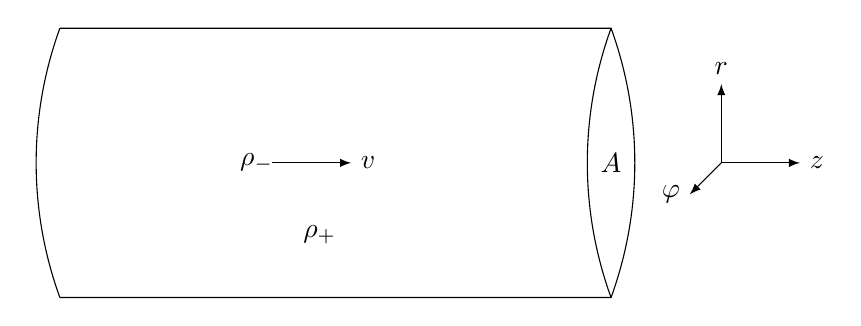
\begin{tikzpicture}
        \draw (0, 0) -- (7, 0) arc (-20:20:5) coordinate (A) -- ++ (-7, 0);
        \draw[xscale=-1] (-7, 0) arc (-20:20:5);
        \draw[xscale=-1] (0, 0) arc (-20:20:5);
        \path (7, 0) -- (A) node[midway] (B) {\(A\)};
        \node at ($(B) - (4.5, 0)$) {\(\rho_-\)};
        \draw[->] ($(B) - (4.3, 0)$) -- ++ (1, 0) node[right] {\(\vv{v}\)};
        \node at (3.3, 0.8) {\(\rho_+\)};
        \draw[->] ($(B) + (1.4, 0)$) -- ++ (1, 0) node[right] {\(\vh{z}\)};
        \draw[->] ($(B) + (1.4, 0)$) -- ++ (-0.4, -0.4) node[left] {\(\vh{\varphi}\)};
        \draw[->] ($(B) + (1.4, 0)$) -- ++ (0, 1) node[above] {\(\vh{r}\)};
    \end{tikzpicture}
    \caption[Feynman's Wire]{Feynman's wire with cross sectional area \(A\) carrying current \(\vv{J} = \rho_-\vv{v}\).}
\end{figure}

We can compute the magnetic field outside of the wire using Amp\`ere's law,
\begin{equation}
    \curl\vv{B} = \frac{1}{c}\vv{J},
\end{equation}
since \(\diffp{\vv{E}}/{t} = 0\) in this scenario.
In order to be useful in this situation we need the integral form of Amp\`ere's law.
For this we introduce an Amp\`erian loop encircling the wire at a distance \(r\), greater than the radius of the wire, and we integrate Amp\`ere's law over a surface bounded by this loop.
The left hand side then becomes
\begin{equation}
    \int_S (\curl\vv{B}) \cdot \dl{\vv{S}} = \oint \vv{B} \cdot \dl{\vv{r}}
\end{equation}
through an application of Stoke's theorem, and the right hand side becomes
\begin{equation}
    \frac{1}{c}\int_S \vv{J} \cdot \dl{\vv{S}} = \frac{1}{c}\rho_-vA,
\end{equation}
where we have used the fact that \(\vv{J}\) is \(\rho_-\vv{v}\) inside the wire and zero outside the wire.

By symmetry we have that \(\vv{B}\) depends only on \(r\), the distance from the centre of the wire.
The right hand rule tells us that \(\vv{B}\) will be in the \(\vh{\varphi}\) direction.
So, \(\vv{B}(\vv{r}) = B(r)\vh{\varphi}\).
Hence we have
\begin{equation}
    \oint \vv{B} \cdot \dl{\vv{r}} = 2\pi r B(r).
\end{equation}
Equating these terms and solving for \(\vv{B}\) we have that
\begin{equation}
    \vv{B}(r) = \frac{\rho_-vA}{2\pi r c}\vh{\varphi}.
\end{equation}
Note that inside the wire the only thing that changes is we replace \(A\) with \(\pi r^2\).
For a neutral wire we have that \(\rho_+ = \rho_0\) and \(\rho_- = -\rho_0\), which allows us to write the magnetic field as
\begin{equation}
    \vv{B} = -\frac{\rho_0vA}{2\pi r c}\vh{\varphi}.
\end{equation}

Suppose we place a small test charge, \(q\), at a distance \(r\) from the wire, such that the test charge also moves with velocity \(\vv{v}\).
The force on this test charge will be
\begin{equation}
    \vv{F} = \frac{q}{c}\vv{v} \times \vv{B} = \frac{q\rho_0A}{2\pi r}\frac{v^2}{c^2}\vh{r}.
\end{equation}
Here we have used the fact that \(\vv{v} = v\vh{z}\) and \(\vh{z} \times \vh{\varphi} = -\vh{r}\).
The result is that the test charge will accelerate radially away from the wire, at least initially.

Suppose now, that we transform to a frame in which the negative charges are stationary.
In this frame the positive charges now move with velocity \(-\vv{v}\).
In the first frame there was a net force on the charge, so we expect there to be a force in this frame also.
However, now that \(q\) is stationary in this frame the magnetic field cannot be the source of this force.
Instead the force is due to the electric field in this frame.
To see this we have to transform the current into our frame.

In the first frame we had
\begin{equation}
    J^\mu = (0, \rho_-\vh{z}).
\end{equation}
Transforming to the new frame with a boost along the \(z\)-axis we get that
\begin{equation}
    c\rho' = \gamma(c\rho - \beta J^z) = -\beta\rho_-v \implies \rho' = \gamma\beta^2\rho_0.
\end{equation}
So, despite being neutral in the first frame we see that the wire is charged in the new frame.
This is because densities are not Lorentz invariant, since volumes are subject to Lorentz contraction.
The result is that there is an electric field in this frame given by
\begin{equation}
    \vv{E}' = \frac{\rho_0 \gamma A}{2\pi r}\frac{v^2}{c^2}\vh{r}.
\end{equation}
This is just the standard electric field for a charged rod,
\begin{equation}
    \vv{E} = \frac{\rho A}{2\pi r}\vh{r},
\end{equation}
which can be derived from Gauss' law.
The force on the test charge is then
\begin{equation}
    \vv{F}' = q\vv{E}' = \gamma\frac{q\rho_0A}{2\pi r}\frac{v^2}{c^2}\vh{r}.
\end{equation}
Note that this force is the same as in the first frame, but with an extra factor of \(\gamma\), since we are using the force here as defined by \(\vv{F} = \diff{\vv{p}}/{t}\), rather than \(\vv{F} = \diff{\vv{p}}/{\tau}\), so the force also changes between frames due to time dilation.
The resulting motion of the test charge will of course be the same regardless of the frame we perform the calculations in.

This example shows the rather remarkable fact that we can turn electric fields into magnetic fields and vice versa by transforming to different frames.
It should be noted that there is still a magnetic field in the second frame, it just has no effect on the particle since it is stationary.
This idea will shortly lead to us combining the electric and magnetic fields into a single object.

\section{Electromagnetic Potentials}
\epigraph{Lorentz and Lorenz. They're different guys. Not that it matters, they're both dead.}{Donal O'Connell}
Recall that in the Lorenz gauge we have
\begin{equation}
    \left( \frac{1}{c^2}\diffp[2]{}{t} - \laplacian \right)\varphi = \rho, \qqand \left( \frac{1}{c^2}\diffp[2]{}{t} - \laplacian \right)\vv{A} = \frac{1}{c}\vv{J}.
\end{equation}
These are simply \cref{eqn:wave equation for scalar potential lorenz gauge,eqn:wave equation for vector potential lorenz gauge}.
We can write these more compactly using the d'Alembertian, \(\partial^2\):
\begin{equation}
    \dalembertian \varphi = \rho = \frac{1}{c}J^0, \qqand \dalembertian \vv{A} = \frac{1}{c}\vv{J} = \frac{1}{c}J^i\ve{i}.
\end{equation}
This suggests that we should define a new quantity \(A^\mu = (\varphi, \vv{A})\), such that
\begin{equation}\label{eqn:wave operator on potential gives current}
    \dalembertian A^\mu = \frac{1}{c}J^\mu.
\end{equation}
Since the right hand side is a contravariant Lorentz vector and the d'Alembertian is a scalar operator the quotient theorem means that \(A^\mu\) is a contravariant Lorentz vector also.
We call \(A^\mu\) the \defineindex{four-potential}, \define{gauge potential}\index{gauge potential|see{four-potential}}, or \define{gauge field}\index{gauge field|see{four-potential}}.

\subsection{Gauge Transformations}
Consider the Lorenz gauge condition,
\begin{equation}
    \frac{1}{c}\diffp{\varphi}{t} + \div\vv{A} = 0.
\end{equation}
We can rewrite this in relativistic notation as
\begin{equation}
    \partial_\mu A^\mu = 0,
\end{equation}
which shows that this gauge condition is Lorentz invariant.
This makes this gauge condition a good choice for our use.
Compare this to the Coulomb gauge condition, \(\div\vv{A} = 0\), which is \emph{not} Lorentz invariant, and so isn't of much use when doing relativistic electrodynamics.

Consider the generic gauge transformations
\begin{equation}
    \varphi \to \varphi' = \varphi - \frac{1}{c}\diffp{\chi}{t}, \qqand \vv{A} \to \vv{A}' = \vv{A} + \grad\chi.
\end{equation}
We can write these in terms of the four-potential as
\begin{equation}
    A^0 \to A'^0 = A^0 - \partial_0\chi, \qqand A^i \to A'^i = A^i + \partial_i\chi.
\end{equation}
The mixture of up and down indices is not good here, we can lower the time indices freely and the spatial indices at the cost of a minus sign giving
\begin{equation*}
    A_0 \to A'_0 = A_0 - \partial_0\chi, \qand -A_i \to -A'_i = -A_i + \partial_i\chi \implies A_i \to A'_i = A_i - \partial_i\chi.
\end{equation*}
We can then combine these into a single Lorentz invariant statement:
\begin{equation}
    A_\mu \to A'_\mu - \partial_\mu\chi.
\end{equation}

\chapter{The Field Tensor}
\section{Electromagnetic Fields}
The electric field is given in terms of the potentials by
\begin{equation}
    \vv{E} = -\frac{1}{c}\diffp{\vv{A}}{t} - \grad\varphi.
\end{equation}
We can write this in terms of components as
\begin{equation}
    E^i = -\frac{1}{c}\diffp{A^i}{t} - \partial_i\varphi = -\partial_0A^i - \partial_iA^0.
\end{equation}
Again, we have mixed up and down indices which we should get rid of:
\begin{equation}
    E^i = -\partial^0A^i + \partial^iA^0.
\end{equation}

The magnetic field is given by
\begin{equation}
    \vv{B} = \curl \vv{A}.
\end{equation}
The components of \(\vv{B}\) are then given by
\begin{align}
    B^1 &= \partial_2A^3 - \partial_3A^2 = -\partial^2A^3 + \partial^3A^2,\\
    B^2 &= \partial_3A^1 - \partial_1A^3 = -\partial^3A^1 + \partial^1A^3,\\
    B^3 &= \partial_1A^2 - \partial_2A^1 = -\partial^1A^2 + \partial^2A^1.\\
\end{align}
Notice how similar the components of both \(\vv{E}\) and \(\vv{B}\) are when written in terms of \(A^\mu\).
Following this similarity we define the quantity
\begin{equation}
    F^{\mu\nu} \coloneqq \partial^\mu A^\mu - \partial^\nu A^\mu,
\end{equation}
which we call the \defineindex{electromagnetic field strength tensor}.
First, notice that \(F^{\mu\nu}\) is an antisymmetric rank 2 tensor, which as given above transforms contravariantly.
Since it is antisymmetric it has at most 6 independent, non-zero components, which just so happen to correspond to the components of \(\vv{E}\) and \(\vv{B}\).
We can easily see from the definition that
\begin{equation}
    F^{i0} = -F^{0i} = E^i.
\end{equation}
A bit more work shows us that the components of \(\vv{B}\) appear in \(F\) through
\begin{align}
    \varepsilon^{ijk}B^k &= \varepsilon^{ijk}(\curl\vv{A})^k\\
    &= \varepsilon^{ijk}\varepsilon^{klm}\partial_lA^m\\
    &= -\varepsilon^{ijk}\varepsilon^{klm}\partial^lA^m\\
    &= -(\delta^{il}\delta^{jm} - \delta^{im}\delta^{jl})\partial^lA^m\\
    &= -\partial^iA^j + \partial^jA^i\\
    &= -F^{ij}.
\end{align}
Since \(F\) is antisymmetric its diagonal vanishes.
Writing out \(F\) in terms of \(E^i\) and \(B^i\) we have
\begin{equation}
    F^{\mu\nu} = 
    \begin{pmatrix}
        0 & -E^1 & -E^2 & -E^3\\
        E^1 & 0 & -B^3 & B^2\\
        E^2 & B^3 & 0 & -B^1\\
        E^3 & -B^2 & B^1 & 0
    \end{pmatrix}
    .
\end{equation}
We can lower indices on \(F^{\mu\nu}\) giving
\begin{align}
    \tensor{F}{_\mu^\nu} &= 
    \begin{pmatrix}
        0 & -E_x & -E_y & -E_z\\
        -E_x & 0 & B_z & -B_y\\
        -E_y & -B_z & 0 & B_x\\
        -E_z & B_y & -B_x & 0
    \end{pmatrix}
    ,\\
    \tensor{F}{^\mu_\nu} &= 
    \begin{pmatrix}
        0 & E_x & E_y & E_z\\
        E_x & 0 & B_z & -B_y\\
        E_y & -B_z & 0 & B_x\\
        E_z & B_y & -B_x & 0
    \end{pmatrix}
    ,\\
    F_{\mu\nu} &=
    \begin{pmatrix}
        0 & E_x & E_y & E_z\\
        -E_x & 0 & -B_z & B_y\\
        -E_y & B_z & 0 & -B_x\\
        -E_z & -B_y & B_x & 0
    \end{pmatrix}
    .
\end{align}
A handy trick for filling in the indices on the \(B\) components of the field strength tensor is that the indices follow sudoku like rules.
For example consider \(F^{21}\).
This cannot be \(B^1\) since \(F^{01} = -E^1\), and it cannot be \(B^2\) since \(F^{20} = E^2\).
So we are left with \(B^3\).
For the sign we still have to consider \(F^{ij} = -\varepsilon^{ijk}B^k\).

\section{Gauge Invariance}
The field strength tensor inherits gauge invariance from the fields.
Consider the gauge transformation \(A_\mu \to A'_\mu - \partial_\chi\), we have
\begin{align}
    F_{\mu\nu} \to F'_{\mu\nu} &= \partial_\mu(A_\nu - \partial_\nu\chi) - \partial_\nu(A_\mu - \partial_\mu\chi)\\
    &= \partial_\mu A_\nu - \partial_\nu A_\mu - \partial_\mu\partial_\nu\chi + \partial_\nu\partial_\mu\chi\\
    &= F_{\mu\nu},
\end{align}
assuming that \(\chi\) is sufficiently smooth for partial derivatives to commute.

\section{Inhomogeneous Maxwell Equations}
Consider the divergence of \(F^{\mu\nu}\):
\begin{equation}
    \partial_{\mu}F^{\mu\nu} = \partial_\mu(\partial^\mu A^\nu - \partial^\nu A^\mu) = \dalembertian A^\nu - \partial^\nu \partial_\mu A^\mu.
\end{equation}
The final term contains \(\partial_\mu A^\mu\), which vanishes in the Lorenz gauge, so in the Lorenz gauge we have that
\begin{equation}
    \partial_\mu F^{\mu\nu} = \dalembertian A^\nu = \frac{1}{c}J^\nu.
\end{equation}
This last equality is \cref{eqn:wave operator on potential gives current}, which is the defining property of \(A^\mu\).

Now, notice that the left hand side is gauge invariant, since \(F^{\mu\nu}\) is gauge invariant.
The right hand side is also gauge invariant, since the gauge transformations effect only the potentials, not the sources, which have physical meaning.
Whenever we have a start and end point that are gauge invariant it doesn't matter if we made a gauge choice in between, and so we have in \emph{all} gauges that
\begin{equation}
    \partial_\mu F^{\mu\nu} = \frac{1}{c}J^\nu.
\end{equation}

This equation immediately implies conservation of current.
Recall that in relativistic notation the continuity equation is \(\partial_\nu J^\nu = 0\), so we take the divergence of \(\partial_\mu F^{\mu\nu}\) to give us
\begin{equation}
    \partial_\nu \partial_\mu F^{\mu\nu} = \frac{1}{c}\partial_\nu J^\nu.
\end{equation}
Now, the left hand side of this is something symmetric in \(\mu\) and \(\nu\), \(\partial_\nu \partial_\mu\), and something antisymmetric in \(\mu\) and \(\nu\), \(F^{\mu\nu}\).
The product therefore vanishes.
This is a general rule, that the product of symmetric and antisymmetric components in the same indices vanishes.
In this case we can prove it by first commuting the derivatives, then swapping the indices on the field tensor giving a negative sign, and then relabelling \(\mu \leftrightarrow \nu\):
\begin{equation}
    \partial_\nu \partial_\mu F^{\mu\nu} = \partial_\mu \partial_\nu F^{\mu\nu} = -\partial_\mu \partial_\nu F^{\nu\mu} \stackrel{\mu \leftrightarrow \nu}{=} -\partial_\nu \partial_\mu F^{\mu\nu}.
\end{equation}
Finally, the only thing equal to its negative is \(0\) so we must have
\begin{equation}
    0 = \partial_\nu \partial_\mu F^{\mu\nu} = \frac{1}{c}\partial_\nu J^\nu \implies \partial_\nu J^\nu = 0.
\end{equation}
So, \(F^{\mu\nu}\) automatically encodes the conservation laws for charge and current.

Now consider again the divergence \(\partial_\mu F^{\mu\nu} = J^\nu/c\).
In order to recover our pre-relativistic-notation equations we should treat time and space separately.
First, consider the case of \(\nu = 0\).
We then have \(J^0/c = \rho\), giving
\begin{equation}
    \partial_\mu F^{\mu0} = \partial_0F^{00} + \partial_iF^{i0} = \partial_iF^{i0} = \partial_iE^i = \div\vv{E}.
\end{equation}
Here we have used the fact that \(F^{00} = 0\) and \(F^{i0} = E^i\).
Combining these results we have
\begin{equation}
    \div\vv{E} = \rho,
\end{equation}
which is Gauss' law.

This time consider \(\nu = i\).
We then have
\begin{align}
    \partial_iF^{\mu i} &= \partial_0 F^{0i} + \partial_jF^{ji}\\
    &= -\partial_0 F^{i0} - \partial_jF^{ij}\\
    &= -\partial_0 E^i + \partial_j\varepsilon^{ijk}B^k\\
    &= -\frac{1}{c}\diffp{E^i}{t} + (\curl\vv{B})^i.
\end{align}
Here we have used antisymmetry: \(F^{\mu\nu} = -F^{\nu\mu}\), and identified the components \(F^{i0} = E^i\) and \(F^{ij} = -\varepsilon^{ijk}B^k\).
We also have \(\partial_iF^{\mu i} = J^i/c\).
Combining these results and rearranging for \(\curl\vv{B}\) we get
\begin{equation}
    \curl\vv{B} = \frac{1}{c}\vv{J} + \frac{1}{c}\diffp{\vv{E}}{t}.
\end{equation}
This is Amp\`ere's law.

\section{Homogeneous Maxwell Equations}
When we introduced the potentials we did so as the solutions to the two homogeneous (source free) Maxwell equations, \(\div\vv{B} = 0\) and \(\curl\vv{E} + c^{-1}\diffp{\vv{B}}/{t} = \vv{0}\).
We therefore look for an equation for which \(F^{\mu\nu}\) is a solution causing the equation to vanish identically.

If we consider the term \(\partial_\mu F^{\mu\nu}\) appearing in the previous section to be the divergence then the fact that both divergences and curls appear in Maxwell's equations suggests that we should look for some curl-like term.
Since the curl has components \(\varepsilon^{ijk}\partial_j V^k\) we will try something similar, say \(\varepsilon^{\mu\nu\alpha\beta}\partial_\mu F_{\alpha\beta}\).
The question is, does this vanish?

Before we answer this question we introduce a new quantity, called the \defineindex{dual field strength tensor}, and defined by
\begin{equation}
    F^*_{\mu\nu} \coloneqq -\frac{1}{2}\varepsilon_{\mu\nu\alpha\beta}F^{\alpha\beta}.
\end{equation}
\begin{ntn}{}{}
    There is not a consistent notation for this quantity.
    Some sources call it \(F^*_{\mu\nu}\), like we have, others use \(G_{\mu\nu}\), or \(\tilde{F}_{\mu\nu}\).
    
    Note that the star is nothing to do with complex conjugates, the field strength tensor is a real quantity.
    Instead we can think of the star as relating to the Hodge star operator, since in the language of differential forms the potential is a one-form, \(A\), the field strength is a two-form, \(F = \dl{A}\), and the dual field strength is its Hodge dual, \(\star F\).
\end{ntn}
We can easily derive the components of the dual field tensor in terms of the potential:
\begin{align}
    F^*_{\mu\nu} &= -\frac{1}{2}\varepsilon_{\mu\nu\alpha\beta}F^{\alpha\beta}\\
    &= -\frac{1}{2}\varepsilon_{\mu\nu\alpha\beta}(\partial^\alpha A^\beta - \partial^\beta A^\alpha)\\
    &= -\frac{1}{2}\varepsilon_{\mu\nu\alpha\beta}\partial^\alpha A^\beta + \frac{1}{2}\varepsilon_{\mu\nu\alpha\beta} \partial^\beta A^\alpha\\
    &= -\frac{1}{2}\varepsilon_{\mu\nu\alpha\beta}\partial^\alpha A^\beta - \frac{1}{2}\varepsilon_{\mu\nu\beta\alpha} \partial^\beta A^\alpha\\
    &= -\varepsilon_{\mu\nu\alpha\beta}\partial^\alpha A^\beta
\end{align}
where in the last step we relabel indices in the second term, \(\alpha \leftrightarrow \beta\), and in the step before that we used the antisymmetry of the Levi-Civita symbol.

Now consider the divergence of the dual field tensor:
\begin{align}
    \partial_\mu F^{*\mu\nu} &= -\frac{1}{2}\partial_\mu \varepsilon^{\mu\nu\alpha\beta}F_{\alpha\beta}\\
    &= -\frac{1}{2}\varepsilon^{\mu\nu\alpha\beta}\partial_\mu F_{\alpha\beta}\\
    &= -\frac{1}{2}\varepsilon^{\mu\nu\alpha\beta}\partial_\mu (\partial_\alpha A_\beta - \partial_\beta A_\alpha)\\
    &= -\frac{1}{2}\varepsilon^{\mu\nu\alpha\beta}\partial_\mu\partial_\alpha A_\beta + \frac{1}{2}\varepsilon^{\mu\nu\alpha\beta}\partial_\mu\partial_\beta A_\alpha\\
    &= 0.
\end{align}
This last equality holds since the partial derivatives are symmetric and the Levi-Civita symbol is antisymmetric, and so their product vanishes.
Hence,
\begin{equation}
    \partial_\mu F^{*\mu\nu} = -\frac{1}{2}\varepsilon^{\mu\nu\alpha\beta}\partial_\mu F_{\alpha\beta} = 0.
\end{equation}

We can fairly easily work out what the components of \(F^*\) are in terms of the electric and magnetic fields.
First, consider the case of \(F^{*i0}\):
\begin{equation}
    F^{*i0} = -\frac{1}{2}\varepsilon^{i0\alpha\beta}F_{\alpha\beta}.
\end{equation}
The non-vanishing terms of this cannot have \(\alpha = 0\) or \(\beta = 0\), so we have that \(\alpha\) and \(\beta\) are spatial indices, and so
\begin{equation}
    F^{*i0} = -\frac{1}{2}\varepsilon^{i0jk}F_{jk}.
\end{equation}
now consider the Levi-Civita symbol.
Swapping the first two indices gives us a negative sign,
\begin{equation}
    F^{*i0} = \frac{1}{2}\varepsilon^{0ijk}F_{jk}.
\end{equation}
Suppose \(ijk = 123\).
Then we have \(\varepsilon^{0123} = -1\), following our convention of \(\varepsilon_{0123} \coloneqq 1\).
This means that \(\varepsilon^{0123} = -\varepsilon^{123}\).
The Levi-Civita symbol is entirely defined by a single value and requiring that it is totally antisymmetric.
This allows us to conclude from this that \(\varepsilon^{0ijk} = -\varepsilon^{ijk}\).
Hence,
\begin{align}
    F^{*0i} &= -\frac{1}{2}\varepsilon^{ijk}F_{jk}\\
    &= \frac{1}{2}\varepsilon^{ijk}\varepsilon^{jkl}B^l,
\end{align}
where we have used the fact that \(F^{jk} = -\varepsilon^{jkl}B^l\).
We now have two options, we can apply an identity for the product of two Levi-Civita symbols, first using the antisymmetry to get the indices to line up with the usual form for the identity:
\begin{align}
    F^{*0i} &= -\frac{1}{2}\varepsilon^{ijk}\varepsilon^{kjl}B^l\\
    &= -\frac{1}{2}(\delta^{ij}\delta^{jl} - \delta^{il}\delta^{jj})B^l\\
    &= -\frac{1}{2}(\delta^{il} - 3\delta^{il})B^l\\
    &= \delta^{il}B^l\\
    &= B^l.
\end{align}
We could also have gotten to the same result by considering \(\varepsilon^{ijk}\varepsilon^{jkl}\) with \(i = 1\), which means that for a non-vanishing term we must have either \(j = 2\) and \(k = 3\), or \(j = 3\) and \(k = 2\).
Either way a non-vanishing result then requires that \(l = 1\).
Doing the same with \(i = 2, 3\) we see that \(i = l\) and the values of \(j\) and \(k\) aren't important for non-vanishing terms and so \(\varepsilon^{ijk}\varepsilon^{jkl} = 2\delta^{il}\).

now consider the components \(F^{*ij}\):
\begin{equation}
    F^{*ij} = -\frac{1}{2}\varepsilon^{ij\alpha\beta}F_{\alpha\beta}.
\end{equation}
In order for this not to vanish either \(\alpha = 0\) or \(\beta = 0\).
Suppose \(\beta = 0\), we can then swap \(\alpha\) and \(\beta\) in both \(\varepsilon^{ij\alpha\beta}\) and \(F_{\alpha\beta}\).
Each swap gives a minus sign, and there are two swaps, so there is no change.
We can then relabel \(\alpha \leftrightarrow \beta\).
Therefore we have two non-zero terms, one with \(\alpha = 0\) and one with \(\beta = 0\), but with the previously mentioned index reshuffling these two terms are actually the same, so we just cancel the factor of \(1/2\).
This gives
\begin{equation}
    F^{*ij} = -\varepsilon^{ij0\beta}F_{0\beta}.
\end{equation}
In order for this not to vanish \(\beta \ne 0\), and so \(\beta\) can be replaced with a spatial index:
\begin{equation}
    F^{*ij} = -\varepsilon^{ij0k}F_{0k}.
\end{equation}
Swapping \(0\) and \(j\) on the Levi-Civita gives a minus sign, which then cancels if we further swap \(0\) and \(i\), that is \(\varepsilon^{ij0k} = -\varepsilon^{i0jk} = \varepsilon^{0ijk} = -\varepsilon^{ijk}\), with the last equality following from the previous logic about four and three index Levi-Civita symbols.
Hence,
\begin{equation}
    F^{*ij} = \varepsilon^{ijk}F_{0k}.
\end{equation}
Now raise the two indices on \(F_{0k}\).
We can raise the \(0\) for free, and raiding the \(k\) introduces a minus sign:
\begin{equation}
    F^{*ij} = -\varepsilon^{ijk}F^{0k}.
\end{equation}
Now, we know \(F^{k0} = E^k\), and \(F^{0k} = -F^{k0}\), so
\begin{equation}
    F^{*ij} = \varepsilon^{ijk}E^k.
\end{equation}

Comparing the components of the two field tensors we have
\begin{alignat}{3}
    F^{*i0} &= B^i, \qquad  & F^{*ij} &= \varepsilon^{ijk}E^k,\\
    F^{i0} &= E^i, \qquad & F^{*ij} &= -\varepsilon^{ijk}B^k.
\end{alignat}
Notice that we can obtain the dual field tensor from the field tensor, \(F \to F^*\), via \(\vv{E} \to \vv{B}\) and \(\vv{B} \to -\vv{E}\).
This is called \defineindex{electromagnetic duality}.
We can view it as a result of Maxwell's equations in a vacuum not distinguishing between the electric and magnetic fields, up to a sign, since we have
\begin{alignat}{3}
    \div\vv{E} &= 0, \qquad & \div\vv{B} &= 0,\\
    \curl\vv{E} &= -\frac{1}{c}\diffp{\vv{B}}{t}, \qquad & \curl\vv{B} &= \frac{1}{c}\diffp{\vv{E}}{t}.
\end{alignat}

\begin{app}{Complex Electromagnetic Field}{}
    One way to make the electromagnetic duality more obvious is to define a complex electromagnetic field
    \begin{equation}
        \symcal{E} \coloneqq \vv{E} + i\vv{B}.
    \end{equation}
    Then the vacuum Maxwell equations can be written compactly as two equations:
    \begin{equation}
        \div\symcal{E} = 0, \qqand \curl \vv{\symcal{E}} = \frac{i}{c}\diffp{\symcal{E}}{t}.
    \end{equation}
    Electromagnetic duality is then expressed by multiplying this quantity by \(-i\):
    \begin{equation}
        -i\symcal{E} = \vv{B} - i\vv{E}.
    \end{equation}
    This is the same result as replacing \(\vv{E}\) with \(\vv{B}\) and \(\vv{B}\) with \(-\vv{E}\).
\end{app}

We can now finally recover the homogenous Maxwell equations.
To do so we consider the divergence of the dual field tensor, which is known to vanish, \(\partial_\mu F^{*\mu\nu} = 0\).
First, consider the case of \(\nu = 0\):
\begin{align}
    0 &= \partial_\mu F^{*\mu0}\\
    &= \partial_0 F^{*00} + \partial_i F^{*i0}\\
    &= \partial_i F^{*i0}\\
    &= \partial_i B^i\\
    &= \div\vv{B}.
\end{align}
Second, consider the case of \(\nu = i\):
\begin{align}
    0 &= \partial_\mu F^{*\mu i}\\
    &= \partial_0 F^{*0i} + \partial_jF^{*ji}\\
    &= -\partial_0 F^{*i0} - \partial_j F^{*ij}\\
    &= -\partial_0 B^i - \partial_j \varepsilon^{ijk}E^k\\
    &= -\frac{1}{c}\diffp{B^i}{t} - (\curl\vv{E})^{i},
\end{align}
which gives Faraday's law:
\begin{equation}
    \curl\vv{E} = -\frac{1}{c}\diffp{\vv{B}}{t}.
\end{equation}

To summarise, the electromagnetic field tensor allows us to write the four Maxwell equations in vector calculus notation as two equations in relativistic notation:
\begin{alignat}{3}
    \partial_\mu F^{\mu\nu} &= \frac{1}{c} J^\nu \qquad && \left\{
    \begin{array}{l}
        \displaystyle \div\vv{E} = \rho,\\
        \displaystyle \curl\vv{B} = \frac{1}{c}\vv{J} + \frac{1}{c}\diffp{\vv{E}}{t},
    \end{array}
    \right.\\
    \partial_\mu F^{*\mu\nu} &= 0 \qquad && \left\{
    \begin{array}{l}
        \displaystyle \div\vv{B} = 0,\\
        \displaystyle \curl\vv{E} = -\frac{1}{c}\diffp{\vv{B}}{t}.
    \end{array}
    \right.
\end{alignat}
Notice that in the absence of sources electromagnetic duality is more obvious:
\begin{equation}
    \partial_\mu F^{\mu\nu} = 0 = \partial_\mu F^{*\mu\nu}.
\end{equation}

\section{Lorentz Transform of the Field Tensor}
The electric and magnetic field are \emph{not} Lorentz vectors, this is because they are really just a neat packaging of components of the electromagnetic field tensor, appropriate for non-relativistic electrodynamics.
The field tensor is a rank 2 contravariant tensor, and so transforms as
\begin{equation}
    F^{\mu\nu} \to F'^{\mu\nu} = \tensor{\Lambda}{^\mu_\alpha} \tensor{\Lambda}{^\nu_\beta} F^{\alpha\beta}.
\end{equation}
Consider a standard Lorentz transformation
\begin{equation}
    \tensor{\Lambda}{^\mu_\nu} = 
    \begin{pmatrix}
        \gamma & -\gamma\beta & 0 & 0\\
        -\gamma\beta & \gamma & 0 & 0\\
        0 & 0 & 1 & 0\\
        0 & 0 & 0 & 1
    \end{pmatrix}
    .
\end{equation}

Consider how the component \(E^1 = F^{10}\) transforms under this Lorentz transformation, in particular we can use the fact that the zeroth and first rows of the standard Lorentz transform are non-zero only in the zeroth and first column.
Hence,
\begin{align}
    E^1 = F^{10} \to F'^{10} &= \tensor{\Lambda}{^1_\alpha} \tensor{\Lambda}{^0_\beta}F^{\alpha\beta}\\
    &= \tensor{\Lambda}{^1_0}\tensor{\Lambda}{^0_0} F^{00} + \tensor{\Lambda}{^1_0}\tensor{\Lambda}{^0_1} F^{01} + \tensor{\Lambda}{^1_1}\tensor{\Lambda}{^0_0} F^{10} + \tensor{\Lambda}{^1_1}\tensor{\Lambda}{^0_1} F^{11}.\notag
\end{align}
We can now use the fact that \(F^{00} = F^{11} = 0\) to further simplify this giving
\begin{align}
    E^1 = F^{10} \to F'^{10} &= \tensor{\Lambda}{^1_0}\tensor{\Lambda}{^0_1} F^{01} + \tensor{\Lambda}{^1_1}\tensor{\Lambda}{^0_0} F^{10}\\
    &= -\tensor{\Lambda}{^1_0} \tensor{\Lambda}{^0_1} F^{10} + \tensor{\Lambda}{^1_1}\tensor{\Lambda}{^0_0}F^{10}\\
    &= \gamma^2(1 - \beta^2)F^{10}\\
    &= E^1,
\end{align}
since \(\gamma^2 = 1/(1 - \beta^2)\).

Now consider \(E^2 = F^{20}\), the transformation coefficient \(\tensor{\Lambda}{^2_\alpha}\) is only non-zero if \(\alpha = 2\), in which case \(\tensor{\Lambda}{^2_2} = 1\) so we have
\begin{align}
    E^2 = F^{20} \to F'^{20} &= \tensor{\Lambda}{^2_\alpha} \tensor{\Lambda}{^0_\beta}F^{\alpha\beta}\\
    &= \tensor{\Lambda}{^2_2}\tensor{\Lambda}{^0_\beta} F^{2\beta}\\
    &= \tensor{\Lambda}{^0_\beta} F^{2\beta}\\
    &= \tensor{\Lambda}{^0_0}F^{20} + \tensor{\Lambda}{^0_1}F^{21}\\
    &= \tensor{\Lambda}{^0_0}E^2 - \tensor{\Lambda}{^0_1}B^3\\
    &= \gamma E^2 - \gamma\beta B^3.
\end{align}
Similarly
\begin{equation}
    E^3 = F^{03} \to F'^{03} = \gamma (E^3 + \beta B^3).
\end{equation}

We can derive the transformation of the magnetic field in the same way, but it is easier to use electromagnetic duality, replacing \(E^i \to B^i\) and \(B^i \to -E^i\), giving
\begin{align}
    B^1 &\to B^1,\\
    B^2 &\to \gamma(B^2 + \beta E^3),\\
    B^3 &\to \gamma(B^3 - \beta E^2).
\end{align}

\subsection{Point Charge}
Consider a point charge, \(q\).
We know that in the rest frame of this charge, \(S'\), the electric field is
\begin{equation}
    \vv{E}'(\vv{r}') = \frac{q}{4\pi r'^3} \vv{r}'
\end{equation}
and the magnetic field is \(\vv{B}'(\vv{r}') = \vv{0}\).
Suppose that in a frame stationary with respect to some observer this particle has velocity \(\vv{v}\).
We want to calculate the values that the observer would measure for the electric and magnetic fields.
We are free to set up the frames such that \(\vv{v} = v\vh{x}\) and at time \(t = 0\) we have the origins of the two frames coincide, this allows us to use standard Lorentz transforms, with the slight change that if the particle has velocity \(\vv{v}\), then the \(S\) frame has velocity \(-\vv{v}\) in frame \(S'\), and so we replace \(\beta\) with \(-\beta\) in our transformations.
For simplicity we only consider the fields at time \(t = 0\).

There are two steps required to calculate the fields the observer measures:
\begin{enumerate}
    \item First, we must Lorentz transform the fields, so \(\vv{E}'(\vv{r}') \to \vv{E}(\vv{r}')\) and \(\vv{B}'(\vv{r}') \to \vv{B}(\vv{r}')\).
    \item Second, we must perform a coordinate transformation to relate positions in the particles rest frame, \(S'\), to positions in the frame at rest relative to the observer, \(S\), so \(\vv{r}' \to \vv{r}\).
\end{enumerate}

First we take the Lorentz transform of the fields.
We'll start with the electric field and come back to the magnetic field later.
We have already seen how the electric field transforms under a standard Lorentz transformation and so we can use this, we just need to be careful to swap \(\beta\) for \(-\beta\).
This gives the components
\begin{align}
    E^1 &= E'^1,\\
    E^2 &= \gamma(E'^2 + \beta B'^3) = \gamma E'^2,\\
    E^3 &= \gamma(E'^3 - \beta B'^2) = \gamma E'^3.
\end{align}
Here we have used the fact that \(B'^i = 0\) for all \(i\).
From this we can fairly easily see that the electric field at position \(\vv{r}'\), as measured in the rest frame of the particle, is
\begin{equation}
    \vv{E}(\vv{r}') = \frac{q}{4\pi r'^3}(x', \gamma y', \gamma z').
\end{equation}

We now need to make a coordinate transformation to express this same value in un-primed coordinates.
This is simple enough for a standard Lorentz transformation, using the fact that we are choosing to have \(t = 0\), we simply have \(x' = \gamma x\), \(y' = y\), and \(z' = z\).
Now consider the value \(r'^2\):
\begin{align}
    r'^2 &= x'^2 + y'^2 + z'^2\\
    &= \gamma^2 x^2 + y^2 + z^2\\
    &= \gamma^2(x^2 + y^2 + z^2) + (1 - \gamma^2)(y^2 + z^2).
\end{align}
To see why this last equality holds just expand it out and it quickly reduces to the previous line.
We can now use
\begin{equation}
    1 - \gamma^2 = 1 - \frac{1}{1 - \beta^2} = \frac{1 - \beta^2}{1 - \beta^2} - \frac{1}{1 - \beta^2} = \frac{1 - \beta^2 - 1}{1 - \beta^2} = -\frac{\beta^2}{1 - \beta^2} = -\beta^2\gamma^2.
\end{equation}
This gives
\begin{align}
    r'^2 &= \gamma^2(x^2 + y^2 + z^2) - \gamma^2\beta^2(y^2 + z^2)\\
    &= \gamma^2r^2 - \gamma^2\beta^2(y^2 + z^2)\\
    &= \gamma^2r^2\left( 1 - \beta^2\frac{y^2 + z^2}{r^2} \right).
\end{align}

\begin{figure}
    \tikzsetnextfilename{point-charge-geometry}
    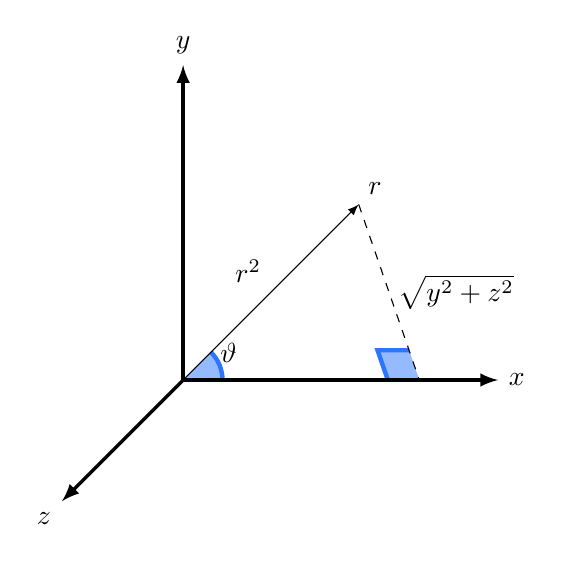
\begin{tikzpicture}
        \path (3, 3, 2) coordinate (C) -- (3, 0, 0) coordinate (A) -- (0, 0, 0) coordinate (B);
        \path pic (theta) [draw=highlight, ultra thick, fill=highlight!50, angle eccentricity=1.25, ""] {angle};
        \node at ($(theta) + (0, 0.1)$) {\(\vartheta\)};
        \path pic [draw=highlight, ultra thick, fill=highlight!50, angle radius=0.4 cm] {right angle=B--A--C};
        \draw[->] (0, 0, 0) -- (3, 3, 2) node[midway, above left] {\(r^2\)} node[above right] {\(\vv{r}\)};
        \draw[dashed] (3, 3, 2) -- (3, 0, 0) node[midway, right] {\(\sqrt{y^2 + z^2}\)} -- (0, 0, 0);
        \draw[very thick, ->] (0, 0) -- (4, 0) node[right] {\(x\)};
        \draw[very thick, ->] (0, 0) -- (0, 4) node[above] {\(y\)};
        \draw[very thick, ->] (0, 0, 0) -- (0, 0, 4) node[below left] {\(z\)};
    \end{tikzpicture}
    \caption{Coordinates for describing a point charge.}
    \label{fig:point charge geometry}
\end{figure}

Now consider the angle \(\vartheta\) defined to be the angle between the position vector, \(\vv{r}\), and the \(x\)-axis.
This is shown in \cref{fig:point charge geometry}.
We can see that the side opposite \(\vartheta\) is \(\sqrt{y^2 + z^2}\), and the hypotenuse is \(r^2\).
Hence,
\begin{equation}
    \sin^2\vartheta = \frac{y^2 + z^2}{r^2}.
\end{equation}
This allows us to write \(r'^2\) in terms of \(\vartheta\):
\begin{equation}
    r'^2  = \gamma^2r^2(1 - \beta^2\sin^2\vartheta).
\end{equation}
For the electric field we actually need the value \(r'^3 = (r'^2)^{3/2}\):
\begin{equation}
    r'^3 = \gamma^3r^3(1 - \beta^2\sin^2\vartheta)^{3/2}.
\end{equation}
The electric field as measured by the observer at position \(\vv{r}\) in their frame is
\begin{equation}
    \vv{E}(\vv{r}) = \frac{q}{4\pi} \frac{1}{\gamma^3r^3(1 - \beta^2\sin^2\vartheta)^{3/2}}(\gamma x, \gamma y, \gamma z) = \frac{q}{4\pi} \frac{1}{\gamma^2r^3(1 - \beta^2\sin^2\vartheta)}\vv{r}.
\end{equation}
Note that the factors of \(\gamma\) for \(x\) comes from the coordinate transformation and the factors of \(\gamma\) for \(y\) and \(z\) come from transforming the field.

Notice that the electric field is still radial, meaning along the \(\vv{r}\) direction.
However, it is no longer spherically symmetric.
For example, if \(\vartheta = 0\) then
\begin{equation}
    \vv{E}(\vv{r}) = \frac{1}{\gamma^2}\frac{q}{4\pi r^3}\vv{r},
\end{equation}
which, for \(\vv{v} \ne \vv{0}\), is lower than the static case since \(\gamma \ge 1\).
On the other hand, for \(\vartheta = \pi/2\) we get a factor of
\begin{equation}
    \gamma^2(1 - \beta^2)^{3/2} = \gamma^2 \gamma^{-3} = \gamma^{-1}.
\end{equation}
So, the electric field is
\begin{equation}
    \vv{E}(\vv{r}) = \gamma\frac{q}{4\pi r^3}\vv{r},
\end{equation}
which is generally greater than in the static case.
The electric field is shown in \cref{fig:moving point charge}.

\begin{figure}
    \tikzsetnextfilename{point-charge-moving-field}
    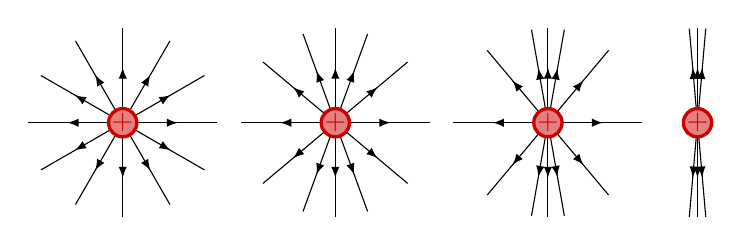
\begin{tikzpicture}
        \foreach \a in {0, 30, ..., 330} {
            \draw[->] (0, 0) -- (\a:0.7);
            \draw (\a:0.65) -- (\a:1.2);
        }
        \node[fill=positive red!50, draw=positive red, very thick, text=positive red, circle, inner sep=0pt] {\(+\)};
        \begin{scope}[xshift=2.7cm]
            \foreach \a in {0, 40, 70, 90, 110, 140, 180, 220, 250, 270, 290, 320} {
                \draw[->] (0, 0) -- (\a:0.7);
                \draw (\a:0.65) -- (\a:1.2);
            }
            \node[fill=positive red!50, draw=positive red, very thick, text=positive red, circle, inner sep=0pt] {\(+\)};
        \end{scope}
        \begin{scope}[xshift=5.4cm]
            \foreach \a in {0, 50, 80, 90, 100, 130, 180, 230, 260, 270, 280, 310} {
                \draw[->] (0, 0) -- (\a:0.7);
                \draw (\a:0.65) -- (\a:1.2);
            }
            \node[fill=positive red!50, draw=positive red, very thick, text=positive red, circle, inner sep=0pt] {\(+\)};
        \end{scope}
        \begin{scope}[xshift=7.3cm]
            \foreach \a in {90, 85, 95, 270, 265, 275} {
                \draw[->] (0, 0) -- (\a:0.7);
                \draw (\a:0.65) -- (\a:1.2);
            }
            \node[fill=positive red!50, draw=positive red, very thick, text=positive red, circle, inner sep=0pt] {\(+\)};
        \end{scope}
    \end{tikzpicture}
    \caption[Electric field of a moving point charge]{The electric field of a moving point charge. The velocity of the point charge increases to the right, and the velocity is to the right. The left most point charge is stationary. As velocity increases the field becomes stronger above and below the charge and weaker in front and behind. In the extreme case of \(v = c\) we get a shock wave, much like a sonic boom.}
    \label{fig:moving point charge}
\end{figure}

We can also compute the magnetic field in the observers frame, since in their frame the charge is moving we expect that the magnetic field will not vanish.
To do so we use the fact that \(\vv{B}' = \vv{0}\).
This allows us to use the relation
\begin{equation}
    \vv{B}' = -\vv{\beta} \times \vv{E}',
\end{equation}
where \(\vv{\beta} = \vv{v}/c\).
This relation holds for a standard Lorentz transformation whenever \(\vv{B} = \vv{0}\).
This is easily shown for a standard Lorentz transformation, simply compute the cross product and show that we recover the known transformation laws for the components of \(\vv{B}\).
In our case we are actually transforming from the primed frame to the un-primed frame, and we have \(-\vv{\beta}\), instead of \(\vv{\beta}\), so
\begin{equation}
    \vv{B} = \vv{\beta} \times \vv{E}.
\end{equation}
We know that \(\vv{E} \propto \vv{r}\), and \(\vv{\beta} \propto \vv{v}\), and so in full we have
\begin{equation}
    \vv{B}(\vv{r}) = \vv{\beta} \times \vv{E} = \frac{q}{4\pi r^2} \frac{1}{\gamma^2(1 - \beta^2\sin^2\vartheta)^{3/2}}\frac{1}{c}\vv{v} \times \vv{r}.
\end{equation}

\section{Field Invariants}
Given a field strength tensor and its dual there are two invariants we can form, \(F^{\mu\nu}F_{\mu\nu}\) and \(F^{\mu\nu}F^*_{\mu\nu}\).
All other combinations, such as \(F^{*\mu\nu}F_{*\mu\nu}\), can be written in terms of these two invariants.
We can evaluate these two invariants fairly easily in terms of the electric and magnetic fields.
First, consider \(F^{\mu\nu}F_{\mu\nu}\):
\begin{align}
    F^{\mu\nu}F_{\mu\nu} &= F^{i0}F_{i0} + F^{0i}F_{0i} + F^{ij}F_{ij}\\
    &= 2F^{i0}F_{i0} + F^{ij}F_{ij}\\
    &= -2F^{i0}F^{i0} + F^{ij}F^{ij}\\
    &= -2E^iE^i + \varepsilon^{ijk}B^k\varepsilon^{ijl}B^l\\
    &= -2\vv{E}^2 + 2\delta^{kl}B^kB^l\\
    &= -2\vv{E}^2 + 2\vv{B}^2.
\end{align}
Here we have used antisymmetry, \(F^{0i}F_{0i} = -F^{i0}F_{0i} = F^{i0}F_{i0}\), raising spatial indices at the cost of a minus sign, \(F^{i0}F_{i0} = -F^{i0}\tensor{F}{^i_0} = -F^{i0}F^{i0}\) and \(F^{ij}F_{ij} = -F^{ij}\tensor{F}{^i_j} = F^{ij}F^{ij}\), the relations \(F^{i0} = E^i\) and \(F^{ij} = -\varepsilon^{ijk}B^k\), and the identity \(\varepsilon^{ijk}\varepsilon^{ijl} = 2\delta^{kl}\).

Similarly we find that
\begin{align}
    F^{\mu\nu}F^*_{\mu\nu} &= F^{i0}F^*_{i0} + F^{0i}F^*_{0i} + F^{ij}F^*_{ij}\\
    &= 2F^{i0}F^*_{i0} + F^{ij}F^*_{ij}\\
    &= -2F^{i0}F^{*i0} + F^{ij}F^{*ij}\\
    &= -2E^iB^i - \varepsilon^{ijk}B^k\varepsilon^{ijl}E^{l}\\
    &= -2\vv{E} \cdot \vv{B} - 2 \delta^{kl}B^kE^l\\
    &= -4\vv{E} \cdot \vv{B}.
\end{align}

These invariants can be used to shortcut having to do full calculations.
For example, if \(\vv{E} \cdot \vv{B} = 0\) in some frame, as is the case for electromagnetic waves, then \(\vv{E} \cdot \vv{B} = 0\) in all frames.
If \(\vv{E}^2 = \vv{B}^2\) in some frame then \(\vv{E}^2 = \vv{B}^2\) in all frames, again this is true for electromagnetic waves.
Further, if \(E < B\) in some frame then \(E > B\) in all frames, and vice versa.

We can also use these invariants to guide which transformations we might consider.
For example, often we want to make a transformation such that one field vanishes in the new frame.
If \(F^{\mu\nu}F_{\mu\nu} > 0\) then this implies that \(B < E\), and so we might look for a frame such that \(\vv{B}\) vanishes.
On the other hand if \(F^{\mu\nu}F_{\mu\nu} < 0\) then \(E < B\) and so we look for a frame in which \(\vv{E}\) vanishes.

\section{Binachi Identity}
The \defineindex{Binachi identity}, is
\begin{equation}
    \partial_\rho F_{\mu\nu} + \partial_\mu F_{\nu\rho} + \partial_\nu F_{\rho\mu} = 0.
\end{equation}
This is easily shown by expanding \(F_{\mu\nu}\) in terms of potentials and using the symmetry of partial derivatives:
\begin{align}
    \partial_\rho F_{\mu\nu} &+ \partial_\mu F_{\nu\rho} + \partial_\nu F_{\rho\mu}\\
    &= \partial_\rho(\partial_\mu A_\nu - \partial_\nu A_\mu) + \partial_\mu (\partial_\nu A_\rho - \partial_\rho A_\nu) + \partial_\nu (\partial_\rho A_\mu - \partial_\mu A_\rho)\\
    &= \textcolor{highlight}{\partial_\rho \partial_\mu A_\nu} - \textcolor{my purple}{\partial_\rho \partial_\nu A_\mu} + \textcolor{my orange}{\partial_\mu \partial_\nu A_\rho} - \textcolor{highlight}{\partial_\mu \partial_\rho A_\nu} + \textcolor{my purple}{\partial_\nu \partial_\rho A_\mu} - \textcolor{my orange}{\partial_\nu \partial_\mu A_\rho}\\
    &= 0.
\end{align}
If we consider the Binachi identity multiplied by \(\varepsilon^{\mu\nu\rho\sigma}\) we find that this implies \(\partial_\mu F^{*ms\nu} = 0\), which is what we started looking for to define \(F^{*\mu\nu}\) in the first place, so we can replace this condition with the Binachi identity if we wish.

\begin{app}{Binachi Identity}{}
    In general relativity there is a similar identity also known as the Binachi identity for the Riemann curvature tensor:
    \begin{equation}
        \nabla_\varepsilon \tensor{R}{^\alpha_{\beta\gamma\delta}} + \nabla_\gamma \tensor{R}{^\alpha_{\beta\delta\varepsilon}} + \nabla_\delta \tensor{R}{^\alpha_{\beta\varepsilon\gamma}} = 0.
    \end{equation}
    Here \(\nabla_\mu\) is a covariant derivative, which reduces to the partial derivative \(\partial_\mu\) in a locally inertial frame.
    The Riemann tensor is defined by
    \begin{equation}
        \tensor{R}{^\alpha_{\beta\gamma\delta}} = \partial_\gamma \tensor{\Gamma}{^\alpha_{\delta\beta}} - \partial_\delta \tensor{\Gamma}{^\alpha_{\gamma\beta}} + \tensor{\Gamma}{^\alpha_{\gamma\mu}}\tensor{\Gamma}{^\mu_{\beta\delta}} - \tensor{\Gamma}{^\alpha_{\delta\mu}}\tensor{\Gamma}{^\mu_{\beta\gamma}}.
    \end{equation}
    Here \(\tensor{\Gamma}{^\alpha_{\beta\gamma}}\) are the affine connections.
    In a locally inertial frame this reduces to
    \begin{equation}
        \tensor{R}{^\alpha_{\beta\gamma\delta}} = \partial_\gamma \tensor{\Gamma}{^\alpha_{\delta\beta}} - \partial_\delta \tensor{\Gamma}{^\alpha_{\gamma\beta}}.
    \end{equation}
    Notice then that if we replace \(\tensor{R}{^\alpha_{\beta\gamma\delta}} \to F_{\alpha\beta}\) and \(\tensor{\Gamma}{^\mu_{\alpha\sigma}} \to A_\alpha\) we get the definition of the field strength tensor.
    
    These two Binachi identities are related by the fact that we can express both the Riemann tensor and the field strength tensor as exterior derivatives.
    For the field strength tensor we have \(F = \dl{A}\), and then we can use the identity \(\symup{d}^2 = 0\) giving \(\dl{F} = \dl{^2A} = 0\).
    For the Riemann tensor the Riemann tensor can be expressed as the exterior derivative of the covariant derivative of a vector field.
\end{app}

\chapter{Energy and Momentum}
\section{Energy--Momentum Tensor}
The \defineindex{energy--momentum tensor}, also called the \define{stress--energy tensor}\index{stress--energy tensor|see{energy--momentum tensor}} is a central object of study in electrodynamics, as well as in wider relativity, including general relativity, where it appears as the source term in Einstein's field equations.
For the purposes of this course we will simply define it and then probe its properties.
One can also derive it as a logical quantity to study based on a few assumptions, or it is possible to derive it entirely from symmetry arguments.

\begin{dfn}{Energy--Momentum Tensor}{}
    The energy--momentum tensor, \(T\), is a rank 2 Lorentz tensor with components
    \begin{equation}
        T_{\mu\nu} \coloneqq \tensor{F}{_\mu^\alpha}\tensor{F}{_{\alpha\nu}} + \frac{1}{4}\eta_{\mu\nu}\tensor{F}{^{\alpha\beta}}\tensor{F}{_{\alpha\beta}}.
    \end{equation}
\end{dfn}
We defined the energy--momentum tensor here in terms of covariant components, but we could equally define it in terms of the contravariant components
\begin{equation}
    T^{\mu\nu} = \tensor{F}{^{\mu\alpha}}\tensor{F}{_\alpha^\nu} + \frac{1}{4}\eta^{\mu\nu}\tensor{F}{^{\alpha\beta}}\tensor{F}{_{\alpha\beta}}.
\end{equation}
Now that we have defined the energy--momentum tensor we will investigate some of its properties.

\subsection{Symmetry}
The energy--momentum tensor is symmetric, that is \(T^{\mu\nu} = T^{\nu\mu}\).
Clearly the second term is symmetric, since the only appearance of \(\mu\) and \(\nu\) is in the metric, \(\eta^{\mu\nu}\), which is symmetric.
For the first term we have
\begin{equation}
    \tensor{F}{_\mu^\alpha} \tensor{F}{_{\alpha\nu}} \to \tensor{F}{_\nu^\alpha}\tensor{F}{_{\alpha\mu}} = \tensor{F}{_{\alpha\mu}}\tensor{F}{_\nu^\alpha} = -\tensor{F}{_{\mu\alpha}}\tensor{F}{_\nu^\alpha} = -\tensor{F}{_\mu^\alpha}\tensor{F}{_{\nu\alpha}} = \tensor{F}{_\mu^\alpha}\tensor{F}{_{\alpha\nu}}.
\end{equation}
Here we have used the antisymmetry of the field tensor, \(F_{\mu\nu} = -F_{\nu\mu}\), as well as the freedom we have to raise an summed index, here \(\alpha\), as long as we lower its pair.
So the first term is also symmetric, and therefore the energy--momentum tensor is symmetric.

\subsection{Trace}
The energy--momentum tensor is traceless, that is \(\tensor{T}{^\mu_\mu} = 0\).
This is simple enough to show, first note that we can write the energy--momentum tensor in a mixed form as
\begin{equation}
    \tensor{T}{^\mu_\nu} = \tensor{F}{^{\mu\alpha}} \tensor{F}{_{\alpha\nu}} + \frac{1}{4}\tensor{\eta}{^\mu_\nu}\tensor{F}{^{\alpha\beta}}\tensor{F}{_{\alpha\beta}}.
\end{equation}
Recall that \(\tensor{\eta}{^\mu_\nu} = \tensor{\delta}{^\mu_\nu}\), and that \(\tensor{\delta}{^\mu_\mu} = 4\) in 4 dimensions.
Hence, the trace of the energy--momentum tensor is
\begin{align}
    \tensor{T}{^\mu_\mu} &= \tensor{F}{^{\mu\alpha}}\tensor{F}{_{\alpha\mu}} + \frac{1}{4}\tensor{\delta}{^\mu_\mu}\tensor{F}{^{\alpha\beta}}\tensor{F}{_{\alpha\beta}}\\
    &= \tensor{F}{^{\mu\alpha}}\tensor{F}{_{\alpha\mu}} + \frac{1}{4}\cdot 4 \tensor{F}{^{\alpha\beta}}\tensor{F}{_{\alpha\beta}}\\
    &= \tensor{F}{^{\mu\alpha}}\tensor{F}{_{\alpha\mu}} + \tensor{F}{^{\alpha\beta}}\tensor{F}{_{\alpha\beta}}\\
    &= -\tensor{F}{^{\mu\alpha}}\tensor{F}{_{\mu\alpha}} + \tensor{F}{^{\alpha\beta}}\tensor{F}{_{\alpha\beta}}\\
    &= 0.
\end{align}
In the last step we can simply relabel \(\alpha \to \mu\) and \(\beta \to \alpha\) in the last term and we see it is the same as the first but with the opposite sign.

\subsection{Components}
We can compute the components of the energy--momentum tensor in terms of the electric and magnetic fields.
This will allow us to prescribe interpretations to these terms.
We will start with the time-time terms, so \(\mu = \nu = 0\).
We have that \(\eta^{00} = 1\), and so
\begin{align}
    T^{00} &= \tensor{F}{^{0\alpha}}\tensor{F}{_\alpha^0} + \frac{1}{4} \tensor{F}{^{\alpha\beta}}\tensor{F}{_{\alpha\beta}}\\
    &= \tensor{F}{^{00}}\tensor{F}{_0^0} + \tensor{F}{^{0i}}\tensor{F}{_i^0} - \frac{1}{2}(\vv{E}^2 - \vv{B}^2)\\
    &= -\tensor{F}{^{0i}}\tensor{F}{^{i0}} - \frac{1}{2}(\vv{E}^2 - \vv{B}^2)\\
    &= \tensor{F}{^{i0}}\tensor{F}{^{i0}} - \frac{1}{2}(\vv{E}^2 - \vv{B}^2)\\
    &= E^iE^i - \frac{1}{2}(\vv{E}^2 - \vv{B}^2)\\
    &= \frac{1}{2}(\vv{E}^2 + \vv{B}^2)\\
    &= u.
\end{align}
Here \(u\) is the energy density of the electromagnetic field.
We have used here the antisymmetry of the electromagnetic field tensor, which implies \(F^{00} = 0\), the fact that raising a spatial index gives a minus sign, the component \(F^{i0} = E^i\), and the field tensor invariant
\begin{equation}
    F^{\mu\nu}F_{\mu\nu} = 2(\vv{B}^2 - \vv{E}^2).
\end{equation}

From this we can see that the interpretation of the time-time component of the energy--momentum tensor is as the energy density of the electromagnetic field.

Next consider the time-space component, so \(\nu = 0\) and \(\mu = i\), or equivalently \(\mu = 0\) and \(\nu = i\) since the energy--momentum tensor is symmetric.
We have
\begin{align}
    T^{i0} &= \tensor{F}{^{i\alpha}}\tensor{F}{_\alpha^0} + \frac{1}{4}\eta^{i0} \tensor{F}{^{\alpha\beta}}\tensor{F}{_{\alpha\beta}}\\
    &= \tensor{F}{^{i0}}\tensor{F}{_0^0} + \tensor{F}{^{ij}}\tensor{F}{_j^0}\\
    &= \tensor{F}{^{i0}}\tensor{F}{^{00}} - \tensor{F}{^{ij}}\tensor{F}{^{j0}}\\
    &= \varepsilon^{ijk}B^kE^j\\
    &= (\vv{E}\times\vv{B})^{i}\\
    &= \frac{1}{c}S^i.
\end{align}
Here \(\vv{S} \coloneqq c\vv{E}\times\vv{B}\) is the Poynting vector.
As well as the previously mentioned properties, we have used the fact that \(\eta\) is diagonal, and the components \(F^{ij} = -\varepsilon^{ijk}B^k\).

From this we can see that the interpretation of the time-space components of the energy--momentum tensor is as the energy density flux.

Finally consider the space-space components, so \(\mu = i\) and \(\nu = j\).
We then have
\begin{align}
    T^{ij} &= \tensor{F}{^{i\alpha}}\tensor{F}{_\alpha^j} + \frac{1}{4}\eta^{ij} \tensor{F}{^{\alpha\beta}}\tensor{F}{_{\alpha\beta}}\\
    &= \tensor{F}{^{i0}}\tensor{F}{_0^j} + \tensor{F}{^{ik}}\tensor{F}{_k^j} + \frac{1}{2}\delta^{ij}(\vv{E}^2 - \vv{B}^2)\\
    &= \tensor{F}{^{i0}}\tensor{F}{^{0j}} - \tensor{F}{^{ik}}\tensor{F}{^{kj}} + \frac{1}{2}\delta^{ij}(\vv{E}^2 - \vv{B}^2)\\
    &= -\tensor{F}{^{i0}}\tensor{F}{^{j0}} - \varepsilon^{ikl}B^l\varepsilon^{kjm}B^m + \frac{1}{2}\delta^{ij}(\vv{E}^2 - \vv{B}^2).
\end{align}
As well as the previously mentioned properties, we have used the fact that \(\eta^{ij} = -\delta^{ij}\).
We now use
\begin{equation}
    \varepsilon^{ikl}\varepsilon^{jkm} = \varepsilon^{ilk}\varepsilon^{kjm} = \delta^{ij}\delta^{lm} - \delta^{im}\delta^{lj}
\end{equation}
and so 
\begin{equation}
    \varepsilon^{ikl}\varepsilon^{jkm}B^lB^m = \vv{B}^2 - B^iB^j.
\end{equation}
Hence,
\begin{align}
    T^{ij} &= -E^iE^j - \vv{B}^{2} - B^iB^j \frac{1}{2}\delta^{ij}(\vv{E}^2 - \vv{B}^2)\\
    &= -\left( E^iE^j + B^iB^j - \frac{1}{2}\delta^{ij}(\vv{E}^2 + \vv{B}^2) \right)\\
    &= - [\text{Maxwell Stress Tensor}]^{ij}.
\end{align}
Here we define the \defineindex{Maxwell stress tensor} as the tensor with components
\begin{equation}
    \sigma_{ij} = E^iE^j + B^iB^j - \frac{1}{2}\delta^{ij}(\vv{E}^2 + \v{B}^2).
\end{equation}
We can think of this as the flux of three--momentum, which also gives us an interpretation of the space-space components of the energy--momentum tensor, and also explains the alternative name of the stress--energy tensor.

\subsection{Divergence}
The divergence of the energy--momentum tensor is fairly easy to compute:
\begin{align}
    \partial_\mu T^{\mu\nu} &= \partial_\mu(\tensor{F}{^{\mu\alpha}} \tensor{F}{_\alpha^\nu}) + \frac{1}{4}\eta^{\mu\nu} \partial_\mu (\tensor{F}{^{\alpha\beta}}\tensor{F}{_{\alpha\beta}})\\
    &= (\partial_\mu\tensor{F}{^{\mu\alpha}})\tensor{F}{_\alpha^\nu} + \tensor{F}{^{\alpha\mu}} \partial_\mu \tensor{F}{_\alpha^\nu} + \frac{1}{4} (\partial^\nu \tensor{F}{^{\alpha\beta}}) \tensor{F}{_{\alpha\beta}} + \frac{1}{4} \tensor{F}{^{\alpha\beta}} \partial^\nu \tensor{F}{_{\alpha\beta}}.
\end{align}
So far this is just the product rule.
In the first term we can identify \(\partial_\mu F^{\mu\alpha} = J^\alpha/c\) as the inhomogeneous Maxwell equation.
In the second term we can lower the \(\alpha\) and \(\mu\) on the first field tensor and raise the \(\mu\) on the derivative and the \(\alpha\)  on the second field tensor, so the second term becomes \(F_{\alpha\mu}\partial^\mu F^{\alpha\nu}\).
In the final term if we lower the \(\alpha\) and \(\beta\) on the first field tensor and raise them on the second then we see that the third and final terms are equal.
Hence,
\begin{align}
    \partial_\mu T^{\mu\nu} &= \frac{1}{c}J^\alpha\tensor{F}{_\alpha^\nu} + \tensor{F}{_{\alpha\mu}}\partial^\mu\tensor{F}{^{\alpha\nu}} + \frac{1}{2}\tensor{F}{_{\alpha\beta}}\partial^\nu \tensor{F}{^{\alpha\beta}}\\
    &= \frac{1}{c}J_\alpha\tensor{F}{^{\alpha\nu}} + \tensor{F}{_{\alpha\mu}}\partial^\mu\tensor{F}{^{\alpha\nu}} + \frac{1}{2}\tensor{F}{_{\alpha\beta}}\partial^\nu \tensor{F}{^{\alpha\beta}}\label{eqn:div energy momentum}
\end{align}
Now consider the final term of this.
We can use the Binachi identity, \(\partial^\nu F^{\alpha\beta} + \partial^\alpha F^{\beta\nu} + \partial^\beta F^{\nu\alpha} = 0\), to rewrite the derivative as \(\partial^\nu F^{\alpha\beta} = -\partial^\alpha F^{\beta\nu} - \partial^\beta F^{\nu\alpha}\).
The final term is therefore
\begin{equation}
    \frac{1}{2}F_{\alpha\beta} \partial^\nu F^{\alpha\beta} = -\frac{1}{2}(F_{\alpha\beta}\partial^\alpha F^{\beta\nu} - F_{\alpha\beta} \partial^\beta F^{\nu\alpha}).
\end{equation}
If we swap \(\alpha \to \mu\) and \(\beta \to \alpha\) in the first term and \(\beta \to \mu\) in the second term then we see both terms here are the same and we are left with \(-F_{\mu\alpha}\partial^\mu F^{\alpha\nu}\), which cancels with the second term in \cref{eqn:div energy momentum}.
Hence,
\begin{equation}
    \partial_\mu T^{\mu\nu} = \frac{1}{c}J_\alpha F^{\alpha\nu}.
\end{equation}

From this we see that the divergence is non-zero when there is a current flow, and hence a flow fo energy/momentum.

Consider the time component of the divergence of the energy--momentum tensor, so \(\nu = 0\).
On the one side we have
\begin{align}
    \partial_\mu T^{\mu0} &= \partial_0T^{00} + \partial_iT^{i0}\\
    &= \frac{1}{c}\diffp{u}{t} + \frac{1}{c}\div\vv{S}.
\end{align}
On the other side we have
\begin{align}
    \frac{1}{c}J_\mu F^{\mu0} = \frac{1}{c}J_0F^{00} + \frac{1}{c}J_iF^{i0} = \frac{1}{c}J_iF^{i0} = -\frac{1}{c}J^iF^{i0} = -\frac{1}{c}J^iE^i = -\frac{1}{c}\vv{J}\cdot\vv{E}.
\end{align}
We can interpret this as the power density, and we have
\begin{equation}
    \diffp{u}{t} + \div\vv{S} = -\vv{J}\cdot\vv{E}.
\end{equation}

Consider instead the space components of the divergence of the energy--momentum tensor, so \(\nu = i\).
We have
\begin{align}
    \frac{1}{c}J_\mu F^{\mu i} &= \frac{1}{c}(J_0F^{0i} + J_jF^{ji})\\
    &= \frac{1}{c}(-J_0F^{i0} - J_jF^{ij})\\
    &= \frac{1}{c}(-J^0F^{i0} + J^jF^{ij})\\
    &= \frac{1}{c}(-J^0E^i - J^j\varepsilon^{ijk}B^k)\\
    &= \frac{1}{c}(-\rho cE^i - (\vv{J}\times\vv{B})^i)\\
    &= -\left( \rho E^i + \frac{1}{c}(\vv{J} \times \vv{B})^i \right)\\
    &= -[\text{Lorentz Force Density}]^i.
\end{align}
So we can interpret this as the force.

This allows us to interpret \(\partial_\mu T^{\mu\nu} = J_\mu F^{\mu\nu}/c\) as a conservation law.
In particular,
\begin{equation}
    \diffp{p_{\symup{em}}^i}{t} + \partial_j T^{ij} = -\diffp{p_{\symup{mech}}^i}{t},
\end{equation}
where \(p_{\symup{em}}^i\) is the three-momentum associated with the electromagnetic fields and \(p_{\symup{mech}}^i\) is the three-momentum associated with the movement of matter, whose rate of change is the force.

\section{Relativistic Point Particle}
Consider a point particle.
We posit that each particle has two associated Lorentz scalars, its mass, \(m\), and its charge, \(q\).
Further the current associated with such a particle is given by \(j^\mu = qu^\mu\), where \(u^\mu = \diff{x^\mu}/{\tau}\) is the four-velocity of the particle.
We therefore have
\begin{equation}
    \frac{1}{c}F^{\mu\nu}j_\nu = \frac{q}{c}F^{\mu\nu}u_\nu.
\end{equation}
The equation of motion is then
\begin{equation}
    \diff{p^\mu}{\tau} = m\diff{u^\mu}{\tau} = m a^\mu = \frac{q}{c}F^{\mu\nu}u_\nu.
\end{equation}

We know that \(u \cdot u = c^2\) is constant and so \(u \cdot a = 0\).
Hence we have
\begin{equation}
    0 = m u\cdot a = \frac{q}{c}u_\mu F^{\mu\nu}u_\nu.
\end{equation}
This is guaranteed to be true by the fact that \(u_\mu u_\nu\) is symmetric in \(\mu\) and \(\nu\) whereas \(F^{\mu\nu}\) is antisymmetric in \(\mu\) and \(\nu\).
This is a good sign that we are going in the correct direction.

Recall that \(u^\mu = (\gamma c, \gamma\vv{v})\), \(\diff{}/{\tau} = \gamma\diff{}/{t}\), and \(p^\mu = (E/c, \vv{p})\).
Consider the \(\mu = 0\) component, we have
\begin{multline}
    \diff{p^0}{\tau} = \frac{\gamma}{c} \diff{E}{t} = \frac{q}{c}F^{0\nu}u_\nu = -\frac{q}{c}F^{\nu0}u_\nu\\
    = -\frac{q}{c}F^{i0}u_i = \frac{q}{c}F^{i0}u^i = \frac{q}{c}E^iu^i = \frac{q}{c}\vv{E}\cdot\vv{v}.
\end{multline}
Now consider the \(\mu = i\) components,
\begin{align}
    \diff{p^i}{\tau} &= \gamma\diff{p^i}{t}\\
    &= \frac{q}{c}F^{i\nu}u_\nu\\
    &= \frac{q}{c}(F^{i0}u_0 + F^{ij}u_j)\\
    &= \frac{q}{c}(E^iu_0 + \varepsilon^{ijk}B^k\gamma v^j)\\
    &= \frac{q}{v}(\gamma cE^i + \gamma(\vv{v}\times\vv{B})^i)\\
    &= q\gamma E^i + \frac{q}{c}\gamma(\vv{v}\times \vv{B})^i.
\end{align}
Hence,
\begin{equation}
    \diffp{\vv{p}}{t} = q\vv{E} + \frac{q}{c}(\vv{v} \times \vv{B}).
\end{equation}
This is exactly the Lorentz force law for a charged particle in an electromagnetic field.
This shows us that we are considering the correct current with \(j_\nu = qu_\nu\).
    
    \part{Action Principles}
    \chapter{Non-Relativistic Actions}
    \epigraph{I got a career out of Taylor expanding.}{Donal O'Connell}
    
    This section will be mostly a review of content covered in other courses, in particular in the Lagrangian dynamics course and the quantum theory course.
    For more on actions and the calculus of variations see the Lagrangian dynamics course and for more on the particular methods used here to find stationary actions see the quantum theory course.
    
    We will introduce the key ideas of action principles through some, hopefully familiar, non-relativistic examples, before we discus relativistic generalisations.
    We start with a very simple example.
    
    \section[Non-Relativistic Point Particle in One Dimension in a Potential][First Example]{Non-Relativistic Point Particle in One Dimension in a Potential}
    Consider a non-relativistic point particle in one dimension in a potential, \(V\), which depends on the position of the particle, \(x\), and nothing else.
    The action for this particle along some path, \(x(t)\), between times \(a\) and \(b\) is defined to be the functional
    \begin{equation}
        S[x(t)] = \int_a^b \left[ \frac{1}{2}m\dot{x} - V(x) \right] \dd{t}.
    \end{equation}
    We consider a small variation, \(x(t) \to x(t) + \delta x(t)\), where \(\delta x(t)\) is small.
    The action on this varied path is
    \begin{align}
        S[x(t) + \delta x(t)] &= \int_a^b \left[ \frac{1}{2}m \left( \diff{}{t} [x(t) + \delta x(t)] \right)^2 - V(x(t) + \delta x(t)) \right] \dd{t} \notag\\
        &= \int_a^b \left[ \frac{1}{2}m\left( \diff{x}{t} + \diff{}{t}\delta x(t) \right)^2 - V(x(t) + \delta x(t)) \right] \dd{t}.
    \end{align}
    Taylor expanding the potential to first order in \(\delta x(t)\), and expanding the brackets, again keeping only terms up to linear order in \(\delta x(t)\) we get
    \begin{equation}
        S[x(t) + \delta x(t)] = \int_a^b \left[ \frac{1}{2}m\dot{x}(t)^2 + m\dot{x} \diff{}{t}\delta x(t) - V(x(t)) - V'(x(t))\delta x(t) \right] \dd{t}.
    \end{equation}
    Carrying around all of this explicit time dependence is getting a bit bothersome, so we'll drop the \((t)\) for \(x\) and \(\delta x\) most of the time:
    \begin{equation}
        S[x + \delta x] = \int_a^b \left[ \frac{1}{2}m \dot{x} + \dot{x} \diff{}{t}\delta x - V(x) - V'(x)\delta x \right] \dd{t}.
    \end{equation}
    Notice that we can write this in terms of the action on the unvaried path, plus some extra terms:
    \begin{equation}
        S[x + \delta x] = S[x] + \int_a^b \left[ m \dot{x} \diff{}{t}\delta x - V'(x)\delta x \right] \dd{t}.
    \end{equation}
    We therefore define the variation in \(S\) due to this variation in the path to be
    \begin{equation}
        \delta S[x(t)] \coloneqq S[x(t) + \delta x(t)] - S[x(t)].
    \end{equation}
    So,
    \begin{equation}\label{eqn:variation in action}
        \delta S[x(t)] = \int_a^b \left[ m \dot{x} \diff{}{t}\delta x - V'(x)\delta x \right] \dd{t}.
    \end{equation}
    
    In order to extract any physics from this variation we need the principle of least action.
    
    \begin{clm}{Principle of Least Action}{}
        The \defineindex{principle of least action}, or more accurately the principle of stationary action, states that the physical trajectory of a particle is such as to minimise the appropriate action.
    \end{clm}
    The phrase \enquote{appropriate action} is quite a lot here, since we usually define the action such that applying the principle of least action gives the correct results, so its a rather circular argument, but it works, and it generalises.
    
    One argument for why the principle of least action applies comes from the path integral formulation of quantum mechanics.
    In this we have an integral of \(\exp(i S[x(t)]/\hbar)\).
    This oscillates a lot, apart from near to where \(S[x(t)]\) is stationary, and so only the stationary path has a meaningful contribution to the integral, with the rapid oscillations cancelling out.
    
    Another thing we need to consider is what it means for a functional to be stationary.
    For a normal function we would simply say that \(\diff{f}/{t} = 0\) if \(f\) is stationary at some value of \(t\).
    Similarly for a functional we say that \(\delta f[x(t)] = 0\) if \(f\) is stationary on some path, \(x(t)\).
    So, the principle of least action simply reduces to looking for \(x(t)\) such that \(\delta S[x(t)] = 0\).
    
    Before we can do this we will need a theorem about integrals.
    
    \begin{thm}{}{}
        Let \(f\) be some sufficiently smooth function.
        If
        \begin{equation}
            \int_a^b f(t) \delta x(t) \dd{t} = 0
        \end{equation}
        for all distributions \(\delta x(t)\) then \(f(t) = 0\) for all \(t \in [a, b]\).
        
        \begin{proof}[\enquote{proof}]
            Let \(\delta x(t) = \delta(t - t_0)\) for some \(t_0 \in [a, b]\).
            Then
            \begin{equation}
                0 = \int_a^b f(t) \delta x(t) \dd{t} = \int_a^b f(t) \delta(t - t_0) \dd{t} = f(t_0).
            \end{equation}
            Hence \(f(t) = 0\) for all \(t \in [a, b]\).
        \end{proof}
    \end{thm}
    
    This theorem can almost be applied to \cref{eqn:variation in action}.
    The problem is that we have a derivative of \(\delta x\), which doesn't work with this theorem.
    The solution is to either integrate by parts\footnote{as demonstrated multiple times in the quantum theory course}, or, equivalently, to massage our statement to allow us to integrate out this derivative.
    To do this we write
    \begin{equation}
        \diff{}{t} (\dot{x} \, \delta x) = \ddot{x} \, \delta x + \dot{x} \diff{}{t}\delta x.
    \end{equation}
    Hence,
    \begin{equation}
        \int_a^b \dot{x}\diff{}{t}\delta x \dd{t} = \int_a^b \left[ \diff{}{t}(\dot{x} \, \delta x) - \ddot{x} \, \delta x \right] \dd{t} = \left[ \dot{x} \, \delta x \right]_a^b - \int_a^b \ddot{x} \, \delta x \dd{t}.
    \end{equation}
    Of course, this is exactly integration by parts, we've just done the middle steps that we usually miss out.
    
    Using this we have
    \begin{align}
        \delta S[x(t)] &= \int_a^b \left[ m\dot{x} \diff{}{t}\delta x - V'(x)\delta x \right]\dd{t}\\
        &= [m\dot{x} \, \delta x(t)]_a^b - \int_a^b [m\ddot{x} + V'(x)]\delta x \dd{t}.
    \end{align}
    Now restrict the variation to be zero on the boundary, so \(\delta x(a) = \delta x(b) = 0\).
    This means that the first term vanishes and we have
    \begin{equation}
        \delta S[x(t)] = -\int_a^b [m \ddot{x} + V'(x)] \delta x \dd{t}.
    \end{equation}
    Imposing the principle of least action and requiring that this holds for any variation with \(\delta x(a) = \delta x(b) = 0\) we have
    \begin{equation}
        0 = \int_a^b [m\ddot{x} + V'(x)] \delta x \dd{t} \implies m\ddot{x} + V'(x) = 0 \implies m\ddot{x} = -V'(x).
    \end{equation}
    Of course, this is just Newton's second law for a particle of mass \(m\) in a potential.
    
    \subsection{The Basic Idea}
    We have seen here all of the basic ideas behind using action principles.
    All that remains is to apply these ideas to more and more complex systems.
    The basic procedure is always the same:
    \begin{enumerate}
        \item Write out the action.
        \item Write out the action on the varied path.
        \item Taylor expand to first order in the variation.
        \item Compute the variation in the action.
        \item Set the variation in the action to zero.
        \item Integrate by parts to get rid of derivatives.
        \item We will be left with something of the form
        \begin{equation}
            \int f(t) \delta x(t) \dd{t} = 0
        \end{equation}
        and requiring that this holds for any variation vanishing on the boundaries means that we must have \(f(t) = 0\) as our equation of motion.
    \end{enumerate}
    
    \subsection{Calculus of Variations}
    We define the variation in something, say \(f(x(t))\), depending on the path \(x(t)\) to be
    \begin{equation}
        \delta f(x(t)) \coloneqq f(x(t) + \delta x(t)) - f(x(t)).
    \end{equation}
    One important example of this is the variation in \(\diff{x}/{t}\):
    \begin{multline}
        \delta \diff{x}{t} = \delta \diff{}{t}(x(t)) = \diff{}{t}(x(t) + \delta x(t)) - \diff{}{t}(x(t))\\
        = \diff{}{t}x(t) + \diff{}{t}\delta x(t) - \diff{}{t} x(t) = \diff{}{t} \delta x(t).
    \end{multline}
    We think of this as meaning that \(\diff{}/{t}\) and \(\delta\) commute, so
    \begin{equation}
        \delta \diff{}{t} = \diff{}{t}\delta.
    \end{equation}
    Similarly one can show that we can exchange the order of variations and integrals.
    
    A fortunate consequence of this is that we can interpret \(\delta \dot{x}\) in two ways, and both are equal.
    Either,
    \begin{equation}
        \delta \dot{x} = \delta (\dot{x}) = \delta \diff{x}{t} = \diff{}{t}\delta x, \qqor \delta \dot{x} = \dot{\delta x} = \diff{}{t} \delta x = \delta \diff{x}{t}.
    \end{equation}
    Since these are equal there is no ambiguity in the notation.
    
    \section[Non-Relativistic General Particle in One Dimension in a Potential][Second Example]{Non-Relativistic General Particle in One Dimension in a Potential}
    A slightly more generic action for a particle in one dimension in some potential is given by defining a \defineindex{Lagrangian}, \(\lagrangian(x(t), \dot{x}(t)) = T - V\), where \(T\) is the kinetic energy of the particle and \(V\) is the potential energy.
    Note that we choose here for the Lagrangian to depend only on the position and velocity of the particle.
    This is not always the case, but often is.
    When this doesn't hold one has to take care with which of the following steps are still valid.
    
    The Lagrangian is defined such that the action is given by its integral:
    \begin{equation}
        S[x(t)] = \int_a^b \lagrangian(x(t), \dot{x}(t)) \dd{t}.
    \end{equation}
    So, we can identify the Lagrangian from the previous example as
    \begin{equation}
        \lagrangian = \frac{1}{2}m\dot{x}^2 - V(x),
    \end{equation}
    which is exactly \(T - V\).
    
    The variation in the action is
    \begin{align}
        \delta S[x(t)] &= \delta \int_a^b \lagrangian(x, \dot{x}) \dd{t}\\
        &= \int_a^b \delta \lagrangian (x, \dot{x})\dd{t}\\
        &= \int_a^b [\lagrangian(x + \delta x, \dot{x} + \delta\dot{x}) - \lagrangian(x, \dot{x})] \dd{t}.
    \end{align}
    To proceed we Taylor expand the Lagrangian to first order in \(\delta x\) and \(\delta \dot{x}\).
    Note that we treat \(x\) and \(\dot{x}\) as independent variables before we find the equations of motion.
    Therefore we simply have a Taylor expansion in two variables:
    \begin{equation}
        \lagrangian(x + \delta x, \dot{x} + \delta\dot{x}) = \lagrangian(x, \dot{x}) + \diffp{\lagrangian}{x}\delta x + \diffp{\lagrangian}{\dot{x}} \delta\dot{x}.
    \end{equation}
    Hence, the variation in the Lagrangian is
    \begin{equation}
        \delta \lagrangian(x, \dot{x}) = \diffp{\lagrangian}{x}\delta x + \diffp{\lagrangian}{\dot{x}}\delta \dot{x},
    \end{equation}
    and the variation in the action is
    \begin{equation}
        \delta S[x(t)] = \int_a^b \left[ \diffp{\lagrangian}{x}\delta x + \diffp{\lagrangian}{\dot{x}}\delta\dot{x} \right]\dd{t}.
    \end{equation}
    In order to deal with the derivative of \(\delta x\) we again integrate by parts, rewriting
    \begin{equation}
        \diff{}{t}\left( \diffp{\lagrangian}{\dot{x}} \delta x \right) = \diffp{\lagrangian}{\dot{x}}\delta\dot{x} + \diff{}{t}\left( \diffp{\lagrangian}{\dot{x}} \right)\delta x
    \end{equation}
    we have
    \begin{align}
        \delta S[x(t)] &= \int_a^b \left[ \diffp{\lagrangian}{x}\delta x + \diff{}{t}\left( \diffp{\lagrangian}{\dot{x}} \delta x \right) - \diff{}{t}\left( \diffp{\lagrangian}{t} \right) \delta x \right] \dd{t}\\
        &= \left[ \diffp{\lagrangian}{\dot{x}} \delta x \right]_a^b + \int_a^b \left[ \diffp{\lagrangian}{x}\delta x - \diff{}{t}\left( \diffp{\lagrangian}{t} \right) \right] \delta x \dd{t}.
    \end{align}
    Again we impose that the variation vanishes at the boundary, so the first term vanishes.
    The principle of least action then gives us
    \begin{equation}
        \diffp{\lagrangian}{x} = \diff{}{t}\diffp{\lagrangian}{\dot{x}}.
    \end{equation}
    This is the \defineindex{Euler--Lagrange equation}.
    
    \subsection{Basic Idea}
    The Euler--Lagrange equation gives us another way to find the physical trajectory.
    If we know the action in the form
    \begin{equation}
        S = \int \lagrangian \dd{t}
    \end{equation}
    then we can get the equations of motion by either
    \begin{itemize}
        \item varying \(S\) and setting the variation to zero, or
        \item solving the Euler--Lagrange equations.
    \end{itemize}
    The first will always work.
    The second requires that we have the right form of the Euler--Lagrange equations for the problem at hand, for example as derived here the standard Euler--Lagrange equation works if the Lagrangian depends on position and velocity, but not if it also depends on acceleration.
    
    \chapter{Relativistic Free Action}
    \section{Motivation}
    In this section we will derive the action and Lagrangian for a free relativistic particle.
    We do so motivated by knowing the equations of motion for such a system are
    \begin{equation}
        m\diff{u^\mu}{\tau} = 0,
    \end{equation}
    where \(u\) is the four-velocity of the particle.
    
    For a free particle the motion, and hence action and Lagrangian, shouldn't depend on the location of the particle, \(x\), which we now take to be the four-position.
    More formally put our system should have translation symmetry.
    Recall that this implies momentum conservation, by Noether's theorem\footnote{See the notes from the Lagrangian dynamics course for details.}, which we would expect since the equation of motion
    \begin{equation}
        0 = m\diff{u^\mu}{\tau} = \diff{p^\mu}{\tau}
    \end{equation}
    can be seen as a statement of conservation of momentum.
    Taking \(x\) to be the four-position if our Lagrangian is independent of \(x\) then it is also time independent, which implies energy conservation, this also follows from the time component of the equation of motion.
    
    Another requirement we impose is that the Lagrangian be Lorentz invariant.
    Strictly all we need is for the action to be Lorentz invariant, but this is almost always achieved by having a Lorentz invariant Lagrangian.
    This restriction is reasonable as the physics of the system should not depend on the frame and we want to derive Lorentz covariant equations of motion.
    
    Recall that in the non-relativistic case a free particle has the Lagrangian
    \begin{equation}
        \lagrangian = \frac{1}{2}m\dot{\vv{x}}\cdot\dot{\vv{x}}.
    \end{equation}
    The obvious choice then is to replace the three-velocity, \(\dot{\vv{x}}\) with the four-velocity, \(u\).
    However, recall that \(u \cdot u = c^2\), so this alone cannot give us the particle dynamics.
    The requirement that the Lagrangian is both Lorentz invariant and position independent is actually quite limiting.
    There are only really three Lorentz scalars from which we can build the Lagrangian.
    They are the mass, \(m\), the speed of light, \(c^2 = u \cdot u\), and the proper time experienced by the particle, \(\tau\).
    Motivated by the non-relativistic case we look for an action of the form
    \begin{equation}
        S[x(t)] = \int_a^b \lagrangian(x(t), x'(t)) \dd{\tau}
    \end{equation}
    where \(x\) is the four-position, \(x'\) the four velocity, and we replace coordinate time, \(t\), with proper time \(\tau\).
    
    The action must have units of energy times time, and the Lagrangian units of energy.
    This restricts the possible ways we can combine these three Lorentz scalars.
    After some thinking one comes to the conclusion that the correct form for the action of a free relativistic particle is
    \begin{equation}
        S[x(t)] = -mc^2 \int_a^b \dl{\tau} \iff \lagrangian = -mc^2.
    \end{equation}
    This is motivated by the fact that it correctly reduces to the non-relativistic result in the non-relativistic limit, and also gives the expected equations of motion in the full relativistic case.
    We will demonstrate this now.
    
    \section{Non-Relativistic Limit}
    The proper time is given by \(\dl{\tau} = \dl{t}/\gamma\).
    In the non-relativistic limit \(v \ll c\), and so we can Taylor expand \(1/\gamma\), giving
    \begin{equation}
        \frac{1}{\gamma} = \sqrt{1 - \frac{v^2}{c^2}} = \left( 1 - \frac{v^2}{c^2} \right)^{1/2} \approx 1 - \frac{1}{2}\frac{v^2}{c^2}.
    \end{equation}
    Hence,
    \begin{align}
        S[x(t)] &= -mc^2\int_a^b \dl{\tau}\\
        &\approx -mc^2 \int_a^b \left( 1 - \frac{1}{2}\frac{v^2}{c^2} \right) \dd{t}\\
        &=\int_a^b \frac{1}{2}mv^2 \dd{t} + \text{constant}.
    \end{align}
    The constant is unimportant for the dynamics of the system and can be neglected\footnote{For a proof of this see the Lagrangian dynamics course. Essentially the Lagrangian is always differentiated when we use it so any constants vanish, this is similar to how we can add a constant to the potential energy by choosing a different place to define as zero.}.
    We see therefore that this choice of relativistic Lagrangian is equivalent to the non-relativistic choice of Lagrangian for a free particle.
    
    \section{Relativistic Equation of Motion}
    We will now derive the relativistic equation of motion by varying \(S\).
    Doing so we have
    \begin{equation}
        \delta S = -mc^2 \delta\int \dl{\tau}.
    \end{equation}
    The interpretation of \(\int \dl{\tau}\) is as the total proper time along the path of the particle through spacetime (i.e., its world line).
    In order to have \(\delta S = 0\), as required by the principle of stationary action we need to extremise the total proper time along the path.
    One way to do this is to take a straight line in spacetime\footnote{This is a geodesic, for more details on geodesics and this approach see the notes from the general relativity course.}.
    This is a global property of the path.
    Equations of motion are typically differential equations, which are local, so we need another way to think about this.
    
    Consider two paths, \(x_1\) and \(x_2\), both starting and ending at the same points.
    We can parametrise each path using the proper time along that path, \(\tau_i\).
    So \(x_i = x_i(\tau_i)\) for \(i = 1, 2\).
    The variation in the action between these two paths is
    \begin{equation}
        \delta S = -mc^2 \left[ \int_{\text{path 1}} \dl{\tau_1} - \int_{\text{path 2}} \dl{\tau_2} \right].
    \end{equation}
    In order to derive the equations of motion we first consider path 2 as a deviation from path 1.
    We then choose to use \(\tau_1\) as a common parameter for both paths, which we can do since we can find consider \(\tau_2\) as a function of \(\tau_1\), \(\tau_2(\tau_1)\).
    We then have\footnote{Don't tell the mathematicians we're treating derivatives as fractions.}
    \begin{equation}
        \diff{\tau_2}{\tau_1} = \diff{\tau_2}{\tau_1} \implies \dl{\tau_2} = \diff{\tau_2}{\tau_1}\dd{\tau_1}.
    \end{equation}
    This allows us to combine the two integrals over the paths into one, giving
    \begin{equation}
        \delta S = -mc^2\int \left[ 1 - \diff{\tau_2}{\tau_1} \right]\dd{\tau_1}.
    \end{equation}
    
    The problem with this approach is that it promotes path 1 above path 2.
    In order to avoid this we introduce some third parameter, \(\lambda\), which parametrise both paths\footnote{Small technicality: the paths must both be monotonic functions of \(\lambda\), so that they don't double back on themselves. Here \(\lambda\) is an affine parameter, for more details see the general relativity course.}, so we consider \(\tau_i\) as a function of \(\lambda\), \(\tau_i(\lambda)\).
    We then have two paths, \(x_1(\lambda)\) and \(x_2(\lambda)\).
    
    Next we need to find a way of writing \(\dl{\tau_i}\) in terms of \(\lambda\).
    To do so we consider the spacetime interval:
    \begin{equation}
        c^2\dd{\tau^2} = \dl{x} \cdot \dl{x} \implies \dl{\tau} = \frac{1}{c}\sqrt{\dl{x}\cdot\dl{x}}.
    \end{equation}
    We can then write \(\dl{x}\) in terms of \(\lambda\) using
    \begin{equation}
        \diff{x}{\lambda} = \diff{x}{\lambda} \implies \dl{x} = \diff{x}{\lambda}\dl{\lambda}.
    \end{equation}
    Factoring the factor of \(\dl{\lambda}\) out of the square root we have
    \begin{equation}
        \dl{\tau} = \frac{1}{c}\sqrt{\diff{x}{\lambda} \cdot \diff{x}{\lambda}} \dd{\lambda}.
    \end{equation}
    Hence, the action can be written in terms of the parameter \(\lambda\) as
    \begin{equation}\label{eqn:relativistic action in terms of lambda}
        S[x(t)] = -mc \int_{\lambda_a}^{\lambda_b} \sqrt{\diff{x}{\lambda} \cdot \diff{x}{\lambda}} \dd{\lambda}.
    \end{equation}
    Here \(\lambda_a\) and \(\lambda_b\) are such that \(\tau_i(\lambda_a) = a\) and \(\tau_i(\lambda_b) = b\) fix the end points of the two paths.
    The Lagrangian parametrised by \(\lambda\) is then
    \begin{equation}
        \lagrangian(x'(\lambda)) = -mc\sqrt{\diff{x}{\lambda}\cdot\diff{x}{\lambda}}.
    \end{equation}

    \subsection{Euler--Lagrange Equations}
    We can now consider a slightly more general Lagrangian with position dependence, which will be useful later, in order to derive the Euler--Lagrange equations for a relativistic particle:
    \begin{equation}
        S[x(t)] = \int_{\lambda_a}^{\lambda_b} \lagrangian(x(\lambda), x'(\lambda)) \dd{\lambda}.
    \end{equation}
    The variation in \(S\) is given by varying the Lagrangian, which is done by Taylor expanding, and then integrating by parts until we can identify the integrand as zero if \(\delta S\) is to vanish.
    Some care must be taken over this since \(x\) is a four-vector, but its pretty much identical to the one-dimensional non-relativistic case:
    \begin{align}
        \delta S[x(t)] &= \int_{\lambda_a}^{\lambda_b} \delta \lagrangian(x(\lambda), x'(\lambda)) \dd{\lambda}\\
        &= \int_{\lambda_a}^{\lambda_b} \left[ \diffp{\lagrangian}{x^\mu}\delta x^\mu + \diffp{\lagrangian}{x'^\mu} \delta x'^\mu \right] \dd{\lambda}\\
        &= \int_{\lambda_a}^{\lambda_b} \left[ \diffp{\lagrangian}{x^\mu} \delta x^\mu + \diff{}{\lambda}\left( \diffp{\lagrangian}{x'^\mu} \delta x^\mu \right) - \diff{}{\lambda}\left( \diffp{\lagrangian}{x'^\mu} \right) \delta x^\mu \right]\dd{\lambda}\\
        &= \left[ \diffp{\lagrangian}{x'^\mu} \delta x^\mu \right]_{\lambda_a}^{\lambda_b} + \int_{\lambda_a}^{\lambda_b} \left[ \diffp{\lagrangian}{x^\mu} - \diff{}{\lambda}\left( \diffp{\lagrangian}{x'^\mu} \right) \right] \delta x^\mu \dd{\lambda}.
    \end{align}
    We require that \(\delta x^\mu\) vanishes on the boundary, so the first term vanishes.
    We further require that this holds for arbitrary \(\delta x^\mu\), and so we have that each component of the square bracket in the integral must vanish independent of the other components giving the Euler Lagrange equations for a relativistic particle:
    \begin{equation}
        \diff{}{\lambda}\diffp{\lagrangian}{x'^\mu} = \diffp{\lagrangian}{x^\mu}.
    \end{equation}
    
    \subsection{Recovering Equations of Motion}
    Finally we are ready to derive the equations of motion for the relativistic particle.
    We go back to the position-independent Lagrangian, \(\lagrangian = -mc\sqrt{x'\cdot x'}\).
    We then have
    \begin{equation}
        \diff{\lagrangian}{x^\mu} = 0 \implies \diff{}{\lambda} \diffp{\lagrangian}{x'^\mu} = 0.
    \end{equation}
    So we need to compute \(\diffp{\lagrangian}/{x'^\mu}\).
    An application of the chain rule gives
    \begin{equation}
        \diffp{\lagrangian}{x'^\mu} = -mc \diffp{}{x'^\mu} \sqrt{x'^\nu x'_\nu} = -\frac{1}{2}\frac{mc}{\sqrt{x'\cdot x'}} \diffp{}{x'^\mu}(x'^\nu x'_\nu).
    \end{equation}

    We can compute this derivative in a fairly straight forward way, we just have to be careful about applying the product rule and matching indices:
    \begin{align}
        \diffp{}{x'^\mu}(x'^\nu x'_\nu) &= \diffp{}{x'^\mu} (x'^\nu \eta_{\nu\rho} x'^\rho)\\
        &= \diffp{x'^\nu}{x'^\mu} \eta_{\nu\rho} x'^\rho + x'^\nu \eta_{\nu\rho} \diffp{x'^\rho}{x'^\mu}\\
        &= \tensor{\delta}{^\nu_\mu} \eta_{\nu\rho} x'^\rho + x'^\nu \eta_{\nu\rho} \tensor{\delta}{^\rho_\mu}\\
        &= \eta_{\mu\rho} x'^\rho + x'^\nu \eta_{\nu\mu}\\
        &= 2\eta_{\mu\nu} x'^\nu\\
        &= 2\eta x'_\mu.
    \end{align}
    Here we renamed \(\rho \to \mu\) and used the symmetry of the metric to combine the two terms into one.
    We therefore have
    \begin{equation}
        \diffp{\lagrangian}{x'^\mu} (x'\cdot x') = 2x'_\mu.
    \end{equation}
    We could probably have guessed this by considering \(\diffp{x^2}/{x} = 2x\) and matching indices, and indeed this is how people usually perform this calculation after some practice.
    
    The result is that
    \begin{equation}
        \diffp{\lagrangian}{x'^\mu} = -\frac{mc x'_\mu}{\sqrt{x'\cdot x'}}.
    \end{equation}
    Hence, the equation of motion is
    \begin{equation}
        \diff{}{\lambda}\left[ \frac{mc}{\sqrt{\diff{x}{\lambda} \cdot \diff{x}{\lambda}}} \diff{x^\mu}{\lambda} \right] = 0
    \end{equation}
    where we have written the derivatives out in full, instead of using primes.
    We have also dropped the negative and raised the index on \(x'_\mu\), since the left hand side is equal to zero, and so the overall sign is not important.
    
    While this looks quite complicated it turns out that it is just a straight line in spacetime.
    The complexity arises because \(\lambda\) may be a fairly complex parametrisation.
    The equation of motion gets significantly more simple if we choose a sensible, simple, parametrisation, such as a proper time.
    
    Now consider a single path and choose to use the proper time along this path as the parameter, so \(\lambda = \tau\).
    For a single path there is no reason not to use the proper time, it was only when comparing paths that this caused problems, since its different for each path.
    We then have that
    \begin{equation}
        \diff{x}{\lambda} = \diff{x}{\tau} = u \implies \diff{x}{\lambda}\cdot\diff{x}{\lambda} = u \cdot u = c^2.
    \end{equation}
    Hence, the equation of motion simplifies to
    \begin{equation}
        \diff{}{\tau}\left[ m\diff{x^\mu}{\tau} \right] = 0 \implies m\diff{u^\mu}{\tau} = 0,
    \end{equation}
    which is exactly the equation of motion that we were looking to find, justifying our choice of action.
    
    \subsection{Reparametrisation Invariance}
    This use of parametrisations can be a bit worrying, after all parametrisation is an arbitrary choice, like a coordinate choice or a choice of units, and so it shouldn't effect the overall result.
    We can quite quickly show that this action is independent of how we parametrise the path.
    
    Suppose we have two parameters, \(\lambda\) and \(\kappa\), we want to show that choosing to parametrise our path with \(\kappa\) leaves the form of the action unchanged.
    To do so we consider \(\kappa\) as a function of \(\lambda\), which must be possible since both parametrise the same path and we can therefore draw a correspondence between them.
    Now that we have \(\kappa = \kappa(\lambda)\) we have
    \begin{equation}
        \diff{\kappa}{\lambda} = \kappa' \implies \dl{\kappa} = \kappa'\dd{\lambda}.
    \end{equation}
    By the chain rule we also have
    \begin{equation}
        \diff{x}{\lambda} = \diff{x}{\kappa}\diff{\kappa}{\lambda}.
    \end{equation}
    Hence, the action is
    \begin{align}
        S &= \int \left[ -mc \sqrt{\diff{x}{\lambda} \cdot \diff{x}{\lambda}} \right] \dd{\lambda}\\
        &= \int \left[ -mc \sqrt{\diff{x}{\kappa} \cdot \diff{x}{\kappa} \left( \diff{\kappa}{\lambda} \right)^2} \right] \frac{1}{\kappa'} \dd{\kappa}\\
        &= \int \left[ -mc \sqrt{\diff{x}{\kappa} \cdot \diff{x}{\kappa}} \right] \dd{\kappa}.
    \end{align}
    So, the form of the action is independent of the choice of parametrisation.
    This is called \defineindex{reparametrisation invariance}.
    
    In particular this invariance means we may as well choose a simple parametrisation, such as proper time, leaving us with a particularly simple form of the action
    \begin{equation}
        S = -mc^2 \int \dd{\tau}.
    \end{equation}
    
    \chapter{Alternative Actions}
    The choice of action is not unique.
    We say that two actions are equivalent if they give the same equations of motion.
    Similarly two Lagrangians are equivalent if they give equivalent actions.
    
    There are some obvious things we can do to Lagrangians to give trivially equivalent actions, first, we can add a constant.
    This has no effect on the equations of motion since we always differentiate the Lagrangian and so this term will vanish in the Euler--Lagrange equations.
    Second, we can add a total derivative term, this will not change the Euler--Lagrange equations either\footnote{For proof see the notes from the Lagrangian dynamics course.}.
    There are also non-trivial changes we can make to the action which still give the same results, including using completely different Lagrangians.
    
    \section{Alternative Relativistic Action}
    For a relativistic particle we ruled out using \(m\dot{x}^2/2\), since \(\dot{x}^2 = c^2\) if we interpret this as a \((3 + 1)\)-dimensional equation.
    However, it turns out that if we take this as the action for a free particle we do actually get the same equations of motion as with the action defined in the previous chapter.
    That is the action in \cref{eqn:relativistic action in terms of lambda} is equivalent to the action
    \begin{equation}
        S_2[x(\tau)] \coloneqq -\int \frac{m}{2}\diff{x^\mu}{\tau} \diff{x_\mu}{\tau} \dd{t},
    \end{equation}
    we simply forget that \(\dot{x}^2 = c^2\) until after we have done the variation.
    We will demonstrate this with an even more general choice of action.
    
    Consider the action
    \begin{equation}
        \tilde{S}[x(\lambda)] \coloneqq \int \left[ -g(\lambda)^{-1} \diff{x^\mu}{\lambda} \diff{x_\mu}{\lambda} - \left( \frac{mc}{2} \right)^2 g(\lambda) \right] \dd{\lambda}.
    \end{equation}
    This has the undetermined quantity \(g(\lambda)\).
    We can place restrictions on this quantity by requiring that this action has reparametrisation invariance.
    That is if we consider some new parameter, \(\tilde{\lambda}\).
    We then have
    \begin{equation}
        \diff{x^\mu}{\lambda} \diff{x_\mu}{\lambda} = \diff{x^\mu}{\tilde{\lambda}} \diff{x_\mu}{\tilde{\lambda}} \left( \diff{\tilde{\lambda}}{\lambda} \right)^2,
    \end{equation}
    and
    \begin{equation}
        \dl{\lambda} = \diff{\lambda}{\tilde{\lambda}}\dd{\tilde{\lambda}}.
    \end{equation}
    Hence, the action can be written as
    \begin{equation}
        \tilde{S}[x(\tilde{\lambda})] = \int \left[ -g(\lambda(\tilde{\lambda}))^{-1} \diff{x^\mu}{\tilde{\lambda}} \diff{x_\mu}{\tilde{\lambda}} \diff{\tilde{\lambda}}{\lambda} - \left( \frac{mc}{2} \right)^2 g(\lambda(\tilde{\lambda})) \diff{\lambda}{\tilde{\lambda}} \right] \dd{\tilde{\lambda}}.
    \end{equation}
    Notice that one factor of \(\diff{\tilde{\lambda}}/{\lambda}\) from the chain rule applied to the derivatives cancels with a factor of \(\diff{\lambda}/{\tilde{\lambda}}\) from the change in the measure.
    Enforcing reparametrisation invariance is then equivalent to requiring that
    \begin{equation}
        \tilde{S}[x(\tilde{\lambda})] = \int\left[ -g(\tilde{\lambda})^{-1} \diff{x^\mu}{\tilde{\lambda}} \diff{x_\mu}{\tilde{\lambda}} - \left( \frac{mc}{2} \right)^2 g(\tilde{\lambda}) \right] \dd{\tilde{\lambda}}.
    \end{equation}
    We can see that this is true so long as
    \begin{equation}
        g(\tilde{\lambda}) = \diff{\lambda}{\tilde{\lambda}} g(\lambda(\tilde{\lambda})).
    \end{equation}
    Note that this means that \(g\) does not transform like a normal scalar function, which would be unchanged under reparametrisation, \(f(\lambda) = f(\tilde{\lambda})\).
    It is perhaps clearer if we write this requirement as
    \begin{equation}
        g(\tilde{\lambda})\dd{\tilde{\lambda}} = g(\lambda) \dd{\lambda}.
    \end{equation}
    This requirement is equivalent to saying that \(g(\lambda)\dd{\lambda}\) is a one-form\footnote{A common abuse of terminology is to call \(g(\lambda)\) alone a one-form.}\footnote{For more on one-forms see the notes from the general relativity course.}.
    
    \subsection{Equations of Motion}
    We can get equations of motion from \(\tilde{S}\) by applying the Euler--Lagrange equations, and treating \(g\) as a degree of freedom, that is we take as the Lagrangian
    \begin{equation}
        \lagrangian\left( x^\mu(\lambda), \diff{x^\mu}{\lambda}, g(\lambda), \diff{g}{\lambda} \right) = -g(\lambda)^{-1} \diff{x^\mu}{\lambda}\diff{x_\mu}{\lambda} - \left( \frac{mc}{2} \right)^2 g(\lambda).
    \end{equation}
    Doing so with \(g\) as our degree of freedom we have
    \begin{equation}
        \diffp{\lagrangian}{\left( \diff{g}{\lambda} \right)} = 0
    \end{equation}
    and so one equation of motion is
    \begin{equation}
        0 = \diffp{\lagrangian}{g} = \frac{1}{g(\lambda)^2} \left( \diff{x}{\lambda} \right)^2 - \left( \frac{mc}{2} \right)^2.
    \end{equation}
    Now taking \(x\) as our degree of freedom we have
    \begin{equation}
        \diff{\lagrangian}{x} = 0
    \end{equation}
    and so
    \begin{equation}
        \diff{}{\lambda}\diffp{\lagrangian}{\left( \diff{x}{\lambda} \right)} = \diff{}{\lambda} \left[ -\frac{1}{g(\lambda)} \diff{x^\mu}{\lambda} \right] = 0
    \end{equation}
    is the other equation of motion.
    
    Consider what happens if we choose \(g(\lambda) = 2/m\).
    We then have that
    \begin{equation}
        \left( \diff{x}{\lambda} \right)^2  = c^2
    \end{equation}
    and our second equation of motion becomes
    \begin{equation}
        \diff{}{\lambda}\left[ -\frac{m}{2} \diff{x^\mu}{\lambda} \right] = 0.
    \end{equation}
    These are exactly the same equations of motion as we got by choosing to take \(\lambda = \tau\) in our original action, hence \(\tilde{S}\) and \(S\) are equivalent actions.
    
    Setting \(g(\lambda) = 2/m\) in \(\tilde{S}\) we get
    \begin{equation}
        \tilde{S} = \int \left[ -\frac{m}{2}\diff{x^\mu}{\lambda}\diff{x_\mu}{\lambda} + \text{constant} \right]\dd{\lambda}
    \end{equation}
    and since the constant can be ignored without changing the equations of motion we see that \(S_2\) is an equivalent action to \(S\) also.
    
    \subsection{Which Action To Choose?}
    So, there are three actions, \(S\), \(S_2\), and \(\tilde{S}\), which all produce the same equations of motion.
    Which should we use?
    The answer depends on what we are trying to do.
    The \enquote{correct} action, with an easy physical interpretation, is \(S\), we simply extremise the length of the world line.
    However, it is often easier to work with \(S_2\), after all it doesn't have a square root in it, we simply have to fix \(u^2 = c^2\) after we've done all of the variation.
    The slightly more general action \(\tilde{S}\) has the advantage that we can use it for massless particles also by taking the limit \(m \to 0\), although we can't then take \(g(\lambda) = 2/m\) (which is equivalent to \(\lambda = \tau\)) but instead pick \(g(\lambda) = \text{constant}\) (which is equivalent to picking some alternative affine parameter instead of \(\tau\)).
    
    \chapter{Action for Electromagnetic Fields}
    In this chapter we will motivate the action for the electromagnetic field.
    First, we motivate the use of a Lagrangian density, then we will study which terms could possible occur in the action if it is to have the desired symmetry, and finally we will demonstrate that we recover the correct equations of motion, namely Maxwell's equations.
    We will start by doing so for a free field with no charges or currents
    
    \section{Lagrangian Density}
    When we considered a particle we found that its action was of the form
    \begin{equation}
        S = \int \lagrangian \dd{\lambda}.
    \end{equation}
    That is an integral of the Lagrangian.
    The Lagrangian in turn depends on \(x^\mu(\lambda)\), the position of the particle, and \(\dot{x}^\mu(\lambda)\), the velocity of the particle, which depend on the single parameter \(\lambda\).
    Hence, there is a single integral.
    
    Now consider a string, it was shown in a tutorial question that the position of the string is described by \(\varphi(x, t)\), which gives the deviation from the equilibrium position of the string at position \(x\) along the string and time \(t\).
    This is equivalent to \(x^\mu(\lambda)\) above, with \(\varphi\) being \(x^\mu\) and both \(x\) and \(t\) being parameters like \(\lambda\).
    This value, \(\varphi\), then evolves under the action
    \begin{equation}
        S[\varphi(x, t)] = \int \left[ \frac{1}{2}\left( \diffp{\varphi}{t} \right)^2 - \frac{Y}{2}\left( \diffp{\varphi}{x} \right)^2 \right] \dd{t} \dd{x}
    \end{equation}
    where \(\mu\) is the mass per unit length and \(Y\) is the spring constant per unit length.
    The important thing here is that the \enquote{path}, \(\varphi\), depends on two parameters and we integrate some Lagrangian-like quantity over both of them to get the action.
    
    Now, consider electromagnetism.
    It will be our general goal to see how \(A^\mu\), the four-potential, transforms.
    In general we will consider cases where \(A^\mu\) depends on the position in spacetime, so we consider it to be a function \(A^\mu(x^0, x^1, x^2, x^3)\).
    We treat \(x^\mu\) as parameters here, so we expect a four-dimensional integral.
    We therefore look for an action of the form
    \begin{equation}
        S[A^\mu(x)] = \int \lagrangianDensity \dd{^4x}.
    \end{equation}
    We call \(\lagrangianDensity\) the \defineindex{Lagrangian density}\footnote{It's very common to just refer to the Lagrangian density as the Lagrangian as well.} since we integrate over space (hence density) to get something (the Lagrangian) which we integrate over time to give the action, that is
    \begin{equation}
        S = \int \lagrangianDensity \dd{^4x} = \int \lagrangianDensity \dd{^3 x} \dd{x^0} = c \int \lagrangian \dd{t}
    \end{equation}
    where we define
    \begin{equation}
        \lagrangian = \int \lagrangianDensity \dd{^3x}.
    \end{equation}
    
    \section{Possible Terms}
    In order to narrow down possibilities for \(\lagrangianDensity\) we need to decide what symmetries it should satisfy.
    First, we would like for \(\lagrangianDensity\) to be \emph{Lorentz invariant}, since this guarantees that the equations of motion will be Lorentz invariant.
    Second, we would like for \(\lagrangianDensity\) to be \emph{gauge invariant}, since this guarantees that the equations of motion will be gauge invariant.
    Third, for a free electromagnetic field we would like for \(\lagrangianDensity\) to be \emph{translation invariant}.
    
    Imposing these symmetries we can narrow down the possible terms in the Lagrangian density.
    First, we expect to have the volume element, \(\dl{^4x}\).
    This Lorentz invariant and is trivially gauge invariant since it doesn't depend on the potential.
    It is also translation invariant, since it doesn't depend on position in flat spacetime.
    Second, we expect the electromagnetic tensor to appear in some way.
    In order for this to happen in a Lorentz invariant way we must some how get a scalar, the most obvious way to do this is \(F_{\mu\nu}F^{\mu\nu}\).
    Since the electromagnetic tensor is gauge invariant this product will also be gauge invariant, and for a free field there is no position dependence so it will be translation invariant.
    Note that \(F^{*}_{\mu\nu}F^{*\mu\nu}\) is simply proportional to \(F_{\mu\nu}F^{\mu\nu}\), so doesn't give us anything new.
    
    There are other possible terms too, for example, \(F^*_{\mu\nu}F^{\mu\nu}\) satisfies these required symmetries.
    However, it doesn't have parity invariance, which it turns out is a required symmetry in electromagnetism.
    Other terms with the required symmetry properties include powers of \(F_{\mu\nu}F^{\mu\nu}\), such as \((F_{\mu\nu}F^{\mu\nu})^2\), and derivatives of the electromagnetic field tensor, such as \(\partial_\rho F_{\mu\nu} \partial^\rho F^{\mu\nu}\).
    However, these terms turn out to be less important in classical electrodynamics and instead appear as higher order corrections in quantum electrodynamics.
    
    \section{Action}
    We need the action to have units of energy times time, or more generally units of \(\hbar\).
    This is fundamentally since the action appears in the path integral
    \begin{equation}
        \int \exp\left[ \frac{i}{\hbar}S \right] \, \symcal{D}x
    \end{equation}
    To which we can apply the stationary phase approximation giving the principle of least action in the first place\footnote{See the notes from the quantum theory course.}.
    
    Recall that \(F_{\mu\nu}F^{\mu\nu} = -2\vv{E}^2 + 2\vv{B}^2\), and that \(u = (\vv{E}^2 + \vv{B}^2)/2\) is the energy density.
    We know therefore that \(F_{\mu\nu}F^{\mu\nu}\) has dimensions of energy per volume, or
    \begin{equation}
        [F_{\mu\nu}F^{\mu\nu}] = [\text{energy density}] = \frac{[\text{energy}]}{[\text{length}]^3}.
    \end{equation}
    Now, integrating over the three spatial dimensions gets rid of the per volume part of these dimensions, leaving us with dimensions of energy, which we then integrate over \(x^0\), to get dimensions of length times density:
    \begin{equation*}
        \left[ \int F_{\mu\nu}F^{\mu\nu} \dd{^4x} \right] = \left[ \int \dl{^4x} \right] \frac{[\text{energy}]}{[\text{length}]^3} = \int [\text{energy}] \dd{x^0} = [\text{energy}][\text{length}].
    \end{equation*}
    So, if we include a factor of \(1/c\) then we will get the desired units:
    \begin{equation*}
        \left[ \frac{1}{c} \int F_{\mu\nu}F^{\mu\nu} \dd{^4x} \right] = \frac{[\text{time}]}{[\text{length}]} [\text{energy}][\text{length}] = [\text{energy}][\text{time}] = [\hbar].
    \end{equation*}
    
    This isn't quite the form of the action, there is a conventional factor of \(-1/4\), so the action is defined as
    \begin{equation}
        S[A^\mu(x)] \coloneqq \frac{1}{c}\int_V \left[ -\frac{1}{4}F_{\mu\nu}F^{\mu\nu} \right] \dd{^4x}
    \end{equation}
    where \(V\) is some four-dimensional volume.
    We then define
    \begin{equation}
        \lagrangianDensity(\partial^\mu A^\nu) = -\frac{1}{4c} F_{\mu\nu}F^{\mu\nu}
    \end{equation}
    for the Lagrangian density.
    
    We can also consider a more general action
    \begin{equation}
        S = \frac{1}{c} \int_V \lagrangianDensity(A^\mu, \partial^\mu A^\nu) \dd{^4x}.
    \end{equation}
    It should be noted that the indices appearing in the argument to \(\lagrangianDensity\) are not meant to represent a particular value, they are simply a reminder that \(A^\mu\) is a four-vector and \(\partial^\mu A^\nu\) is a rank 2 tensor.
    This is known as abstract index notation, as opposed to Ricci calculus which we have mostly been using so far, where each index is simply a place holder for a particular coordinate.
    
    \section{Equations of Motion}
    \epigraph{I'm just some guy, you have to wonder why you want to believe me.}{Donal O'Connell}
    Consider the more general action defined above.
    We will vary the potential in order to find the equations of motion:
    \begin{equation}
        A_\mu(x) \to A_\mu(x) + \delta A_\mu(x).
    \end{equation}
    We choose the variation so that, as usual, it vanishes on the boundary of \(V\), denoted \(\partial V\).
    The variation in the action is then
    \begin{align}
        \delta S &= \frac{1}{c} \int_V \delta \lagrangianDensity(A^\mu, \partial^\mu A^\nu) \dd{^4x}\\
        &= \frac{1}{c} \int_V \left[ \diffp{\lagrangianDensity}{A^\mu} \delta A^\mu + \diffp{\lagrangianDensity}{(\partial^\mu A^\nu)} \delta \partial^\mu A^\nu \right] \dd{^4x}.
    \end{align}
    We get this result by simply Taylor expanding in the two variables, \(A^\mu\) and \(\partial^\mu A^\nu\), it just looks a bit weird since one is written as a derivative, and we're actually packaging 20 terms into two with sums over repeated indices.
    
    We apply the usual manipulation of writing the second term, with the variation of a derivative, as the derivative of a product minus the extra term this produces:
    \begin{equation}
        S = \frac{1}{c} \int_V \left[ \diffp{\lagrangianDensity}{A^\mu} \delta A^\mu + \partial^\mu\left( \diffp{\lagrangianDensity}{(\partial^\mu A^\nu)} \delta A^\nu \right) - \partial^\mu\diffp{\lagrangianDensity}{(\partial^\mu A^\nu)} \delta A^\nu \right] \dd{^4x}.
    \end{equation}
    Now consider the term with derivative of the product:
    \begin{equation}
        \int_V \partial^\mu \left( \diffp{\lagrangianDensity}{(\partial^\mu A^\nu)} \delta A^\nu \right) \dd{^4x}.
    \end{equation}
    This is simply the divergence theorem in four dimensions:
    \begin{equation}
        \int_V \div \vv{v} \dd{^d x} = \int_{\partial V} \vv{v} \cdot \dd{\vv{S}} \iff \int_V \partial^\mu v_\mu \dd{^dx} = \int_{\partial V} v_\mu \dd{S}^\mu.
    \end{equation}
    Hence, applying the divergence theorem we have
    \begin{equation}
        \int_V \partial^\mu\left( \diffp{\lagrangianDensity}{(\partial^\mu A^\nu)} \delta A^\nu \right) \dd{^4x} = \int_{\partial V} \diffp{\lagrangianDensity}{(\partial^\mu A^\nu)} \delta A^\nu \dd{S^\mu}.
    \end{equation}
    However, since \(\delta A^\nu\) vanishes on \(\partial V\) this integral is identically zero and so this term does not contribute to the action.
    
    The variation in the action is therefore
    \begin{equation}
        \delta S = \frac{1}{c} \int_V \left[ \diffp{\lagrangianDensity}{A^\mu} \delta A^\mu - \partial^\mu \diffp{\lagrangianDensity}{(\partial^\mu A^\nu)} \delta A^\nu \right] \dd{^4x}.
    \end{equation}
    We can reindex the first term, replacing \(\mu\) with \(\nu\), to get a factor of \(\delta A^\nu\) in both terms which we then factor out:
    \begin{equation}
        \delta S = \frac{1}{c} \int_V \left[ \diffp{\lagrangianDensity}{A^\nu} - \partial^\mu \diffp{\lagrangianDensity}{(\partial^\mu A^\nu)} \right] \delta A^\nu \dd{^4x}.
    \end{equation}
    Hence, requiring that \(\delta S = 0\) according to the principle of least action and taking \(\delta A^\nu\) to be arbitrary, other than the requirement of vanishing on \(\partial V\), we must have that the square brackets vanish, giving the Euler--Lagrange equations for this form of Lagrangian:
    \begin{equation}
        \diffp{\lagrangianDensity}{A^\nu} = \partial^\mu \diffp{\lagrangianDensity}{(\partial^\mu A^\nu)}.
    \end{equation}
    
    Finally, we return to the case of
    \begin{equation}
        \lagrangianDensity = -\frac{1}{4}F^{\mu\nu}F_{\mu\nu}.
    \end{equation}
    Recalling that \(F^{\mu\nu}\) is defined in terms of \(\partial^\mu A^\nu\), and doesn't depend on \(A^\mu\) alone we have
    \begin{equation}
        \diffp{\lagrangianDensity}{A^\nu} = 0.
    \end{equation}
    We can also calculate the other side of the Euler--Lagrange equations fairly easily, we just have to be careful to avoid index clash.
    We start with
    \begin{equation}
        \diffp{\lagrangianDensity}{(\partial^\mu A^\nu)} = -\frac{1}{4}\diffp{}{(\partial^\mu A^\nu)} (F_{\alpha\beta}F^{\alpha\beta}) = -\frac{1}{2} F_{\alpha\beta} \diffp{}{(\partial^\mu A^\nu)} F^{\alpha\beta}
    \end{equation}
    where we have used the freedom in raising and lowering paired indices to notice that both terms in the product rule will give the same result.
    We need only then compute the derivative once, which we do by plugging in the definition for \(F^{\alpha\beta}\):
    \begin{equation}
        \diffp{}{(\partial^\mu A^\nu)} F^{\alpha\beta} = \diffp{}{(\partial^\mu A^\nu)} [\partial^\alpha A^\beta - \partial^\beta A^\alpha].
    \end{equation}
    Now notice that the derivative will vanish on each term, apart from when the indices match up correctly across both the derivatives and the potentials, in which case we get unity.
    Hence,
    \begin{equation}
        \diffp{}{(\partial^\mu A^\nu)} F^{\alpha\beta} = \tensor{\delta}{^\alpha_\mu} \tensor{\delta}{^\beta_\nu} - \tensor{\delta}{^\beta_\mu} \tensor{\delta}{^\alpha_\nu}.
    \end{equation}
    Going back to one side of the Euler--Lagrange equations we have
    \begin{align}
        \diffp{\lagrangianDensity}{(\partial^\mu A^\nu)} &= -\frac{1}{2}F_{\alpha\beta}[\tensor{\delta}{^\alpha_\mu}\tensor{\delta}{^\beta_\nu} - \tensor{\delta}{^\beta_\mu} \tensor{\delta}{^\alpha_\nu}]\\
        &= -\frac{1}{2}[F_{\mu\nu} - F_{\nu\mu}]\\
        &= -F_{\mu\nu},
    \end{align}
    where we have used the antisymmetry of the electromagnetic tensor in the last step.
    
    Hence, the full Euler--Lagrange equations give
    \begin{equation}\label{eqn:free field eom}
        0 = \partial^\mu \diffp{\lagrangianDensity}{(\partial^\mu A^\nu)} = -\partial^\mu F_{\mu\nu}.
    \end{equation}
    This is exactly the Maxwell equation for a free electromagnetic field: \(\partial^\mu F_{\mu\nu} = 0\).
    This justifies our choice of the action, including neglecting higher order terms.
    
    \chapter{Interactions}
    \section{Action for A Current}
    Suppose we have a current density, \(J^\mu(x)\), we can modify our action for the free electromagnetic field by adding an extra interaction term.
    The resulting action is
    \begin{align}
        S &= \frac{1}{c} \int \left[ -\frac{1}{4}F^{\mu\nu}F_{\mu\nu} - \frac{1}{c}J^\mu A_\mu \right] \dd{^4x}\\
        &= \frac{1}{c} \int \left[ -\frac{1}{4}F^{\mu\nu}F_{\mu\nu} \right] \dd{^4x} + \frac{1}{c} \int \left[ -\frac{1}{c} J^\mu A_\mu \right] \dd{^4x}\\
        &= S_{\text{free}} + S_{\text{int}}.
    \end{align}
    In terms of the Lagrangian density we have
    \begin{align}
        \lagrangianDensity &= -\frac{1}{4}F^{\mu\nu}F_{\mu\nu} - \frac{1}{c}J^\mu A_\mu\\
        &= \lagrangianDensity_{\text{free}} + \lagrangianDensity_{\text{int}}.
    \end{align}
    
    \section{Dimensions}
    The first step in justifying this choice is to check it works dimensionally.
    In order to do this it is sufficient to show that \(\lagrangianDensity_{\text{int}}\) has the same dimensions as \(\lagrangianDensity_{\text{free}}\).
    We can also ignore any indices, since they don't change the dimensions.
    That is, we want to show that \([FF] = [JA/c]\).
    To do this we use the fact that \(F^{\mu\nu}\) is defined in terms of derivatives of \(A^\mu\), so \([F] = [\partial A] = \dimension{L}^{-1}[A]\).
    Hence, \([FF] = \dimension{L}^{-1}[FA] = \dimension{L}^{-1}[A][F]\).
    We also know that \(c\) is a speed, so \([JA/c] = \dimension{L}^{-1}\dimension{T}[JA] = \dimension{L}^{-1}[A]\dimension{T}[J]\).
    So, things work out dimensionally as long as \(\dimension{T}[J] = [F]\).
    Recall that Maxwell's equation gives us \(\partial^\mu F_{\mu\nu} = J_\nu/c\), and so we have \([\partial F] = \dimension{L}^{-1}[F] = [J/c] = \dimension{L}^{-1}\dimension{T}[J]\).
    Thus, \([F] = \dimension{T}[J]\), and so the dimensions work.
    
    \section{Equations of Motion}
    The next step in justifying this choice is to show that we get the correct equations of motion, both for the fields and for particles.
    We'll start with the field.
    
    \subsection{Equations of Motion for the Field}
    The Euler--Lagrange equations for a Lagrangian density of the form \(\lagrangianDensity(A^\mu, \partial^\mu A^\nu)\) are
    \begin{equation}
        \partial^\mu \diffp{\lagrangianDensity}{(\partial^\mu A^\nu)} = \diffp{\lagrangianDensity}{A^\nu}.
    \end{equation}
    Since the interaction term doesn't introduce any derivatives of \(A^\mu\) we know from \cref{eqn:free field eom} that
    \begin{equation}
        \partial^\mu \diffp{\lagrangianDensity}{(\partial^\mu A^\nu)} = -\partial^\mu F_{\mu\nu}.
    \end{equation}
    However, the interaction term introduces a term with \(A^\mu\), so the other side of the Euler--Lagrange equations no longer vanishes.
    Instead,
    \begin{align}
        \diffp{\lagrangianDensity}{A^\nu} &= \diffp{}{A^\nu} \left[ -\frac{1}{c}J^\mu A_\mu \right]\\
        &= -\frac{1}{c}\diffp{}{A^\nu} J^\mu A_\mu\\
        &= -\frac{1}{c}\diffp{}{A^\nu} J_\mu A^\mu\\
        &= -\frac{1}{c}J_\mu \diffp{A^\mu}{A^\nu}\\
        &= -\frac{1}{c}J_\mu \tensor{\delta}{^\mu_\nu}\\
        &= -\frac{1}{c}J_\nu.
    \end{align}
    Hence, we have the equation of motion for the fields given by
    \begin{equation}
        \partial^\mu F_{\mu\nu} = \frac{1}{c}J_\nu,
    \end{equation}
    which is exactly the inhomogeneous Maxwell equation.
    
    At this point one might wonder how to derive the homogeneous Maxwell equation, \(\partial^\mu F^*_{\mu\nu} = 0\).
    The answer is that we don't really need to do this because we have used \(F^{\mu\nu} = \partial^\mu A^\nu - \partial^\nu A^\mu\) as a definition and this makes the homogeneous Maxwell equation trivially true.
    The two Maxwell equations aren't on quite the same footing in terms of importance, the inhomogeneous one contains most of the physics.
    This is similar to how the divergence equations in the non-relativistic version are not strictly necessary, since they follow from the curl equations and the identity \(\div\curl\vv{V} = 0\).
    On the physics side we can view this as being a consequence of the fact that it is \(A^\mu\), not \(F^{\mu\nu}\), which is the fundamental variable appearing, for example, in the path integrals of QFT.
    
    \subsection{Gauge Invariance}
    \epigraph{It's actually very interesting, well, I say very interesting. I very quickly get interested in things like this. That's why I'm here.}{Donal O'Connel}
    When justifying the choice of the free action we said that we were looking for something gauge invariant, and we found it by working with the gauge invariant electromagnetic field tensor.
    The interaction term has an explicit \(A_\mu\), which is not manifestly gauge invariant.
    Recall that a gauge transform takes the form of \(A_\mu(x) \to A'_\mu(x) = A_\mu(x) + \partial_\mu \chi(x)\), for some smooth scalar field \(\chi\).
    Using this we can show that the action is gauge invariant:
    \begin{align}
        S_{\text{int}} &\to \frac{1}{c}\int \left[ -\frac{1}{c} J^\mu(A_\mu + \partial_\mu \chi) \right] \dd{^4x}\\
        &= S_{\text{int}} - \frac{1}{c^2} \int \left[ J^\mu \partial_\mu \chi \right] \dd{^4x}\\
        &= S_{\text{int}} - \frac{1}{c^2} \int \left[  \partial_\mu(J^\mu \chi) - (\partial_\mu J^\mu)\chi \right] \dd{^4x}.
    \end{align}

    Now, considering the first term we see that an application of the divergence theorem gives
    \begin{equation}
        \int_{V} \partial_\mu(J^\mu \chi) \dd{^4x} = \int_{\partial V} J^\mu \chi \dd{S_\mu}
    \end{equation}
    where \(S_\mu\) is a normal vector to the boundary \(\partial V\).
    Now, whenever we vary the action we always do so in such a way that variations on the boundary vanish, and hence this term doesn't contribute to the variation, and so doesn't effect the equations of motion.
    
    The second term has \(\partial_\mu J^\mu\), which vanishes by the continuity equation if \(J^\mu\) is a conserved current.
    This hints at a link between the symmetry of gauge invariance and the conservation of current, which is a consequence of Noether's theorem.
    
    The result is that while the action is not strictly gauge invariant the variation in the action is gauge invariant, and that's all we care about.
    More formally the action is gauge invariant up to a surface term if the current is conserved.
    
    At this point we note that often we use terminology inherited from Lagrangian dynamics.
    In particular we might call \(A^\mu\) a generalised coordinate, and the quantity
    \begin{equation}
        \diffp{\lagrangianDensity}{(\partial^\mu A^\nu)}
    \end{equation}
    is the canonical momentum conjugate to \(A^\mu\).
    
    \subsection{Relativistic Interacting Point Particle}
    We have seen that we get the inhomogeneous Maxwell equation as the equation of motion of the field.
    Before we accept this form of the action we should show that it also recovers the correct particle dynamics, namely the Lorentz force law.
    
    Suppose we have some particle of mass \(m\) and charge \(q\).
    The four current splits into a temporal part and spatial part according to \(J^\mu(x) = (\rho(x)c, \vv{J}(x))\).
    For a point particle the charge density is simply a Dirac delta distribution,
    \begin{equation}
        \rho(x) = q \delta^3(\vv{x} - \vv{r}(t)).
    \end{equation}
    The superscript 3 is because this is a delta distribution in three dimensions.
    The charge density depends on the four-position, \(x^\mu = (ct, \vv{x})\).
    This is the four-position of the point at which we are measuring the charge density, not the position of the particle, which is \(r^\mu = (ct', \vv{r})\).
    The spatial part of the current density for a moving charge distribution is \(\vv{J}(x) = \rho(x)\vv{v}(t)\).
    Therefore we can write the four-current as
    \begin{equation}
        J^\mu(x) = q\delta^3(\vv{x} - \vv{r}(t))(c, \vv{v}(t))^\mu.
    \end{equation}
    
    This is not manifestly Lorentz covariant, but we know that \(J^\mu\) is a contravariant four-vector, and so we should be able to massage this into a form making it manifestly Lorentz covariant.
    The first step is to get rid of the three-dimensional Dirac delta in favour for a four dimensional one.
    We can do this by using the fact that if we integrate a four-dimensional delta distribution over time we are left with a three-dimensional spatial delta-distribution.
    Let's introduce \(r^0(t') = ct'\) as the time component of the particle's four-position.
    We therefore have
    \begin{align}
        J^\mu(x) &= q \delta^3(\vv{x} - \vv{r}(t))(c, \vv{v}(t))^\mu\\
        &= q \int \dl{(ct')} \, \delta(ct - ct') \delta^3(\vv{x} - \vv{r}(t')) \diff{r^\mu(t')}{t'}\\
        &= qc \int \dl{t'} \, \delta^4(x - r(t')) \diff{r^\mu}{t'}.
    \end{align}
    Here we have written the four-velocity of the particle as a derivative of its four-position.
    We can choose to use the proper time of the particle as the time parameter, and we therefore get
    \begin{equation}
        J^\mu(x) = qc \int \dl{\tau} \diff{r^\mu}{\tau} \delta^4(x - r(\tau)).
    \end{equation}
    It should be noted that a change of variables (\enquote{cancelling} the \(\dl{\tau}\) in the derivative with the measure of the integral) gives us
    \begin{equation}
        J^\mu(x) = qc \int \dl{r^\mu} \, \delta^4(x - r).
    \end{equation}
    Either of these two forms is manifestly Lorentz covariant, which is what we wanted.
    
    Now consider the total action of the fields and the particle, this can be written as
    \begin{equation}
        S_{\text{tot}} = \frac{1}{c}\int \left[ -\frac{1}{4}F^{\mu\nu}F_{\mu\nu} \right] \dd{^4x} - mc \int \sqrt{\diff{r}{\lambda} \cdot \diff{r}{\lambda}} \dd{\lambda} + \frac{1}{c} \int \left[ -\frac{1}{c}J^\mu A_\mu \right] \dd{^4x}.
    \end{equation}
    The first term is the action for a free electromagnetic field, the second term the action for a free particle, and the third accounts for the interactions between the field and the particle.
    It is this interacting term that we are interested in.
    In more detail we can write it as
    \begin{align}
        S_{\text{int}} &= \frac{1}{c}\int \dl{^4x} \, \left[ -\frac{1}{c}J^\mu A_\mu \right]\\
        &= -\frac{1}{c} \int \dl{^4x} \, qc \int \dl{\tau} \, \diff{r^\mu}{\tau} \delta^4(x - r(t)) A_\mu(x)\\
        &= -\frac{q}{c} \int \dl{\tau} \, \diff{r^\mu}{\tau} A_\mu(r(\tau)).
    \end{align}
    In the last step we swapped the integrals to perform the integral over \(\dl{^4x}\) first using the sifting property of the delta distribution.
    This leaves us with a term which depends on the four-potential at the position of the particle, this means that there is no interaction at a distance, which is what we would expect.
    
    We can reparametrise the interaction action as
    \begin{equation}
        S_{\text{int}} = -\frac{q}{c} \int \dl{\lambda} \, \diff{r^\mu(\lambda)}{\lambda} A_\mu(r(\lambda)).
    \end{equation}
    The total action is then
    \begin{equation}
        S_{\text{tot}} = \frac{1}{c}\int \dl{^4x}\, \left[ -\frac{1}{4}F^{\mu\nu}F_{\mu\nu} \right] -mc \int \dl{\lambda} \, \sqrt{\diff{r}{\lambda} \cdot \diff{r}{\lambda}} - \frac{q}{c} \int \dl{\lambda} \, \diff{r^\mu}{\lambda} A_\mu(r(\lambda)).
    \end{equation}
    
    We can then find the equations of motion for the particle using the appropriate Euler-Lagrange equations, namely
    \begin{equation}
        \diff{}{\lambda} \diff{\lagrangian}{(\diff{r^\mu}{\lambda})} = \diff{\lagrangian}{r^\mu}
    \end{equation}
    where \(\lagrangian\) is the integrand of the total action after performing all spatial integrals.
    There is no dependence on \(r^\mu\) or \(\diff{r^\mu}/{\lambda}\) in the first term, so it doesn't contribute to the particle's equations of motion, which makes sense as that term is only to do with the electromagnetic field.
    
    Performing the derivative of \(\lagrangian\) we have
    \begin{equation}
        \diffp{}{\lambda} \left[ -mc \frac{1}{\sqrt{\diff{r}{\lambda} \cdot \diff{r}{\lambda}}} \diff{r^\mu}{\lambda} - \frac{q}{c}A^\mu(r(\lambda)) \right] = -\frac{q}{c} \diff{r_\nu}{\lambda} \partial^\mu A^\nu(r(\lambda)).
    \end{equation}
    Taking \(\lambda = \tau\) again we have that \((\diff{r}/{\tau})^2 = c^2\), and so computing the derivative with respect to \(\lambda\) we are left with
    \begin{equation}
        -m\diff[2]{r^\mu}{\tau} - \frac{q}{c}\partial^\nu A^\mu(r(\tau)) \diff{r_\nu}{\tau} = -\frac{q}{c}\partial^\mu A^\nu(r(\tau)) \diff{r_\nu}{\tau}.
    \end{equation}
    Collecting the derivatives of the potential together we see that we get the electromagnetic tensor and are left with the final equation of motion
    \begin{equation}
        m \diff[2]{r^\mu}{\tau} = \frac{q}{c}F^{\mu\nu}(r(\tau)) \diff{r_\nu}{\tau}.
    \end{equation}
    We can then identify the left hand side as the four-force and the whole equation is the Lorentz force law, in a covariant form.
    
    We have seen two forms of the total action here.
    The second one, with the interaction in terms of \(\lambda\), is good for deriving the particle's equation of motion.
    The first form, with the interaction in terms of the position, is better for the equations of motion of the field.
    These are unaffected by the particle's presence since \(A^\mu\) and its derivative don't appear in the action for the free particle.
    
    \backmatter
%    \renewcommand{\glossaryname}{Acronyms}
%    \printglossary[acronym]
    \printindex
\end{document}